\documentclass{beamer}

% \setbeamerfont{frametitle}{size=\scriptsize}
\setbeamerfont{framesubtitle}{size=\large}

% \usetheme{PaloAlto}
% \usetheme{Berkeley}
\usetheme{Rochester}

% Font
\usepackage{fontspec}
\setmainfont[Script=Greek]{GFS Artemisia}
\setsansfont[Script=Greek]{GFS Neohellenic}
\setmonofont[Script=Greek]{Noto Mono}

% English-Greek use
\usepackage{polyglossia}
% \setmainlanguage{english}
% \setotherlanguage{greek}
\setmainlanguage{greek}
\setotherlanguage{english}

% \newfontfamily\greekfont{GFS Artemisia}
% \let\greekfonttt\ttfamily

\usepackage{amsmath}
\DeclareMathOperator*{\argmin}{\arg\!\min}
\newcommand{\argminUnder}{\arg\!\min}
\newcommand{\argminB}{\mathop{\mathrm{argmin}}}
\usepackage{mathtools}
\DeclarePairedDelimiter\abs{\lvert}{\rvert}
% \DeclarePairedDelimiter\norm{\lVert}{\rVert}
\newcommand\norm[1]{\left\lVert#1\right\rVert}

% For bold
\usepackage{bm}

% R symbol
\usepackage{amssymb}
\newcommand{\R}{\mathbb{R}}

% Multirow tables
\usepackage{multirow}

% Images
\usepackage{graphicx}
\graphicspath{{./images/}}
\usepackage[font={footnotesize,it}]{caption}
\usepackage[font={footnotesize}]{subcaption}
\renewcommand{\thesubfigure}{\Roman{subfigure}}
\usepackage{float}

% Top right logo
\usepackage{eso-pic}
\newcommand\AtPagemyUpperLeft[1]{\AtPageLowerLeft{%
\put(\LenToUnit{0.88\paperwidth},\LenToUnit{0.85\paperheight}){#1}}}
\AddToShipoutPictureFG{
% \AtPagemyUpperLeft{{
\includegraphics[width=1.3cm,keepaspectratio]{LogoAUTH72ppi.png}}}
\AtPagemyUpperLeft{{
\includegraphics[width=1.3cm,keepaspectratio]{LogoAUTHblack72ppi.png}}}
}

\title[Short title] {Κατάτμηση MRI εικόνων γονάτου με χρήση τεχνικών αραιής
αναπαράστασης}

\institute 
{
    Αριστοτέλειο Πανεπιστήμιο Θεσσαλονίκης \\
    Τμήμα Ηλεκτρολόγων Μηχανικών και Μηχανικών Υπολογιστών \\
    Τομέας Ηλεκτρονικής και Υπολογιστών
}

\author {Κωστινούδης Ευάγγελος}

% \logo{
\includegraphics[height=2.0cm]{LogoAUTH72ppi.png}}
% \titlegraphic{
\includegraphics[height=2cm]{LogoAUTH72ppi.png}}

\date{Απρίλιος 2021}

\makeatletter
\setbeamertemplate{title page} 
{
\vbox{}
% {\usebeamercolor[fg]{titlegraphic}\inserttitlegraphic\par}

{\hfill\usebeamercolor[fg]{titlegraphic}\inserttitlegraphic}
  \begin{centering}
    \begin{beamercolorbox}[sep=8pt,center]{institute}
      \usebeamerfont{institute}\insertinstitute
    \end{beamercolorbox}
    \begin{beamercolorbox}[sep=8pt,center]{title}
      \usebeamerfont{title}\inserttitle\par%
      \ifx\insertsubtitle\@empty%
      \else%
        \vskip0.25em%
        {\usebeamerfont{subtitle} \usebeamercolor[fg]{subtitle} \insertsubtitle\par}%
      \fi%

    \end{beamercolorbox}%
    \vskip1em\par
    \begin{beamercolorbox}[sep=8pt,center]{author}
      \usebeamerfont{author}\insertauthor
    \end{beamercolorbox}

    \small
    \begin{tabular}[t]{@{}l@{\hspace{2pt}}p{.32\textwidth}@{}}
        Επιβλέποντες: & \\
        Καθηγητής: & Θεοχάρης Ιωάννης \\
        Υποψήφιος Διδάκτορας: & Χαδουλός Χρήστος
    \end{tabular}

    \vfill
    \begin{beamercolorbox}[sep=7pt,center]{date}
      \usebeamerfont{date}\insertdate
    \end{beamercolorbox}%\vskip0.5em
  \end{centering}
}

\begin{document}

\begin{frame}

\maketitle

% \begin{tabular}[t]{@{}l@{\hspace{3pt}}p{.32\textwidth}@{}}
%     Επιβλέπων & & \\
%     & Καθηγητής: & Θεοχάρης Ιωάννης \\
%     & Υποψήφιος Διδάκτορας: & Χαδουλός Χρήστος
% \end{tabular}

\end{frame}

\begin{frame}
\frametitle{Δομή παρουσίασης}
\tableofcontents[hideallsubsections]
\end{frame}

\section{Εισαγωγή}

\begin{frame}
% \frametitle{Ορισμοί (1/2)}
\frametitle{Ορισμοί}
\begin{block}{Κατάτμηση (Segmentaion)}
Η κατάτμηση είναι η διαδικασία διαμέρισης μίας εικόνας σε διάφορα ουσιαστικά
τμήματα. Σκοπός της κατάτμησης είναι η απλοποίηση ή/και η αλλαγή της
αναπαράστασης της εικόνας σε κάτι που είναι πιο σημασιολογικά σημαντικό και
είναι πιο εύκολο να αναλυθεί.
\end{block} \pause

\begin{block}{Κατάτμηση βάση ατλάντων}
Η κατάτμηση απεικονίσεων βάση ατλάντων αποτελεί την διαδικασία κατά την οποία
χρησιμοποιούνται απεικονίσεις που έχουν κατανεμηθεί από κάποιον ειδικό, ούτως
ώστε να επιτευχθεί η κατάτμηση της νέας απεικόνισης.
\end{block} 
\end{frame}

\begin{frame}
% \frametitle{Ορισμοί (2/2)}
\frametitle{Αντικείμενο της διπλωματικής}
\begin{block}{Αντικείμενο διπλωματικής}
Στην διπλωματική εργασία εφαρμόστηκαν μέθοδοι κατάτμησης ιατρικών απεικονίσεων
βάση ατλάντων με χρήση μηχανικής μάθησης. Οι απεικονίσεις αφορούν μαγνητικές
τομογραφίες σε γόνατα και οι περιοχές κατάτμησης αποτελούνται από τους
αρθρικούς χόνδρους και τα οστά. Τα δεδομένα που χρησιμοποιήθηκαν προέρχονται
από το Osteoarthritis Initiative Zuse Institute Berlin (OAI ZIB).
\end{block}

\begin{figure}[H]
    \centering

    \begin{subfigure}[t]{0.22\linewidth}
    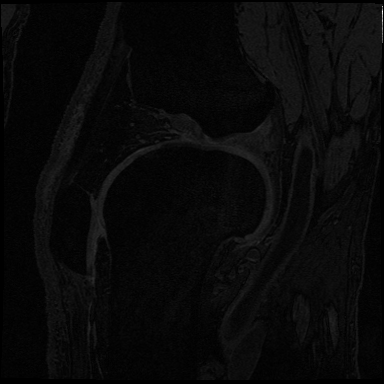
\includegraphics[width=\linewidth]{original_1.png}
    \caption{Απεικόνιση}
    \end{subfigure}
    \begin{subfigure}[t]{0.22\linewidth}
    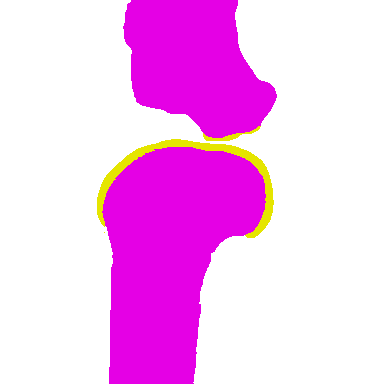
\includegraphics[width=\linewidth]{original_label_registration_1.png}
    \caption{Ετικέτες}
    \end{subfigure}

    \caption{Απεικόνιση και οι αντίστοιχες ετικέτες.}
    \label{fig:image_labels:1}
\end{figure}

\end{frame}

% new section

\begin{frame}
\frametitle{Σύνοψη της διαδικασίας της κατάτμησης}
\begin{enumerate}
    \item<1-> Προεπεξεργασίας δεδομένων.Σκοπός της προεπεξεργασίας είναι να
        παραχθεί μία νέα απεικόνιση που θα έχει καλύτερα αποτελέσματα στην
        μάθηση από αυτά της αρχικής.
    \item<2-> Καταχώρηση (registration) ατλάντων. Η διαδικασία μετασχηματισμού
        διαφορετικών δεδομένων σε ένα σύστημα συντεταγμένων. Η διαδικασία αυτή
        επιδιώκει μέσω του μετασχηματισμού αυτού, την επικάλυψη των κοινών
        χαρακτηριστικών των δεδομένων.
    \item<3-> Επιλογή ατλάντων για την κατάτμηση.
    \item<4-> Κατάτμηση.
\end{enumerate}
\end{frame}


\section{Μεθοδολογία}
\subsection{Προεπεξεργασία δεδομένων}


\iffalse
\begin{frame}
\frametitle{Προεπεξεργασία δεδομένων}
\begin{enumerate}
    \item<1-> Απαλοιφή θορύβου απεικόνισης μέσω ροής της καμπυλότητας (curvature
        flow).
    \begin{equation*} \label{eq:curvature_flow:1}
        I_t = \kappa \abs{\nabla I}
        \text{ όπου }
        \kappa = \frac {\norm{\bm{\gamma}' \times \bm{\gamma}''}}
                       {\norm{\bm{\gamma}'}^3}
    \end{equation*}

    Για $t=0.04$ και 10 επαναλήψεις.

    \item<2-> Αντιστοίχιση ιστογράμματος (histogram matching).

    \begin{figure}[H]
        \centering
        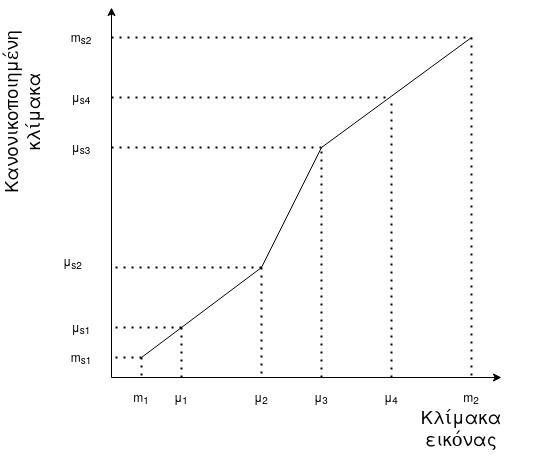
\includegraphics[width=0.3\textwidth]{histogram_matching_2}
        \caption{Γραμμικός μετασχηματισμός αντιστοίχισης ιστογράμματος μίας εικόνας
                 για τέσσερα άκρα.}
        \label{fig:histogram_matching}
\end{figure}
\end{enumerate}

\end{frame}
\fi

\begin{frame}
\frametitle{Προεπεξεργασία δεδομένων}
\framesubtitle{Απαλοιφή θορύβου απεικόνισης μέσω ροής της καμπυλότητας
    (curvature flow)}

Οι ισοστάθμισες καμπύλες (καμπύλες που σχηματίζονται από τα εικονοστοιχεία που
έχουν την ίδια φωτεινότητα) εξελίσσονται μέσω της μερικής διαφορικής εξίσωσης:

\begin{equation*} \label{eq:curvature_flow:1}
    I_t = \kappa \abs{\nabla I}
    \text{ όπου }
    \kappa = \frac {\norm{\bm{\gamma}' \times \bm{\gamma}''}}
                   {\norm{\bm{\gamma}'}^3}
\end{equation*}

Χρησιμοποιείται η τιμή $t=0.04$ και επαναλαμβάνεται 10 φορές.

\begin{figure}[H]
    \centering

    \begin{subfigure}[t]{0.2\linewidth}
    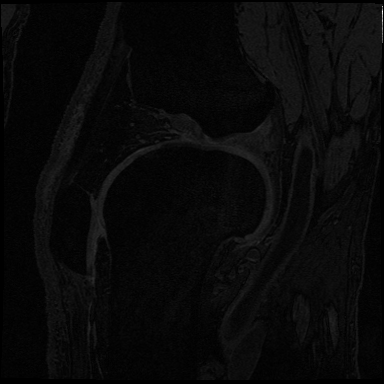
\includegraphics[width=\linewidth]{original_1.png}
    \caption{Αρχική απεικόνιση}
    \end{subfigure}
    \begin{subfigure}[t]{0.2\linewidth}
    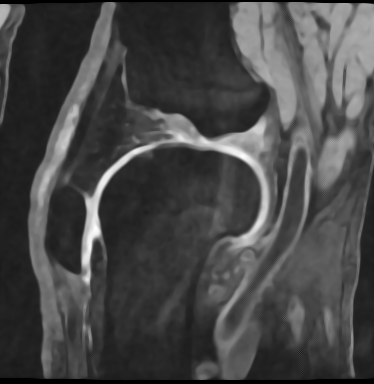
\includegraphics[width=\linewidth]{curvature_1.png}
    \caption{Απεικόνιση με απαλοιφή θορύβου}
    \end{subfigure}

    \iffalse
    \caption{Τομή απεικόνισης γονάτου χωρίς και με την χρήση της απαλοιφής
    θορύβου μέσω ροής της καμπυλότητας.}
    \fi
    \label{fig:curvature_flow:1}
\end{figure}

\end{frame}


\begin{frame}
\frametitle{Προεπεξεργασία δεδομένων}
\framesubtitle{Αντιστοίχιση ιστογράμματος (histogram matching)}

Αντιστοιχίζει το ιστόγραμμα της σταθερής απεικόνισης με το ιστόγραμμα της
κινούμενης.

\begin{figure}[H]
    \centering
    \begin{subfigure}[t]{0.4\linewidth}
    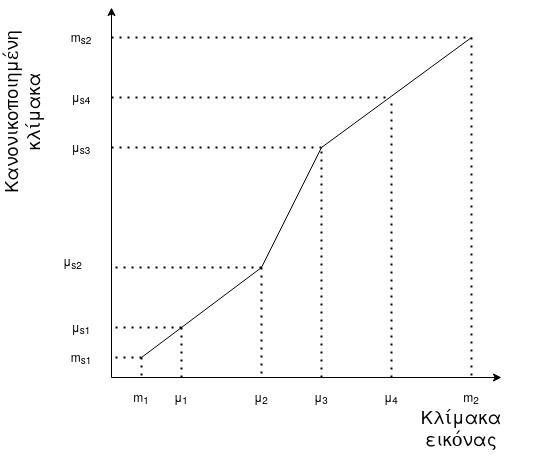
\includegraphics[width=\textwidth]{histogram_matching_2}
    \caption{Γραμμικός μετασχηματισμός αντιστοίχισης ιστογράμματος μίας εικόνας
             για τέσσερα άκρα.}
    \end{subfigure}
    \begin{subfigure}[t]{0.4\linewidth}
    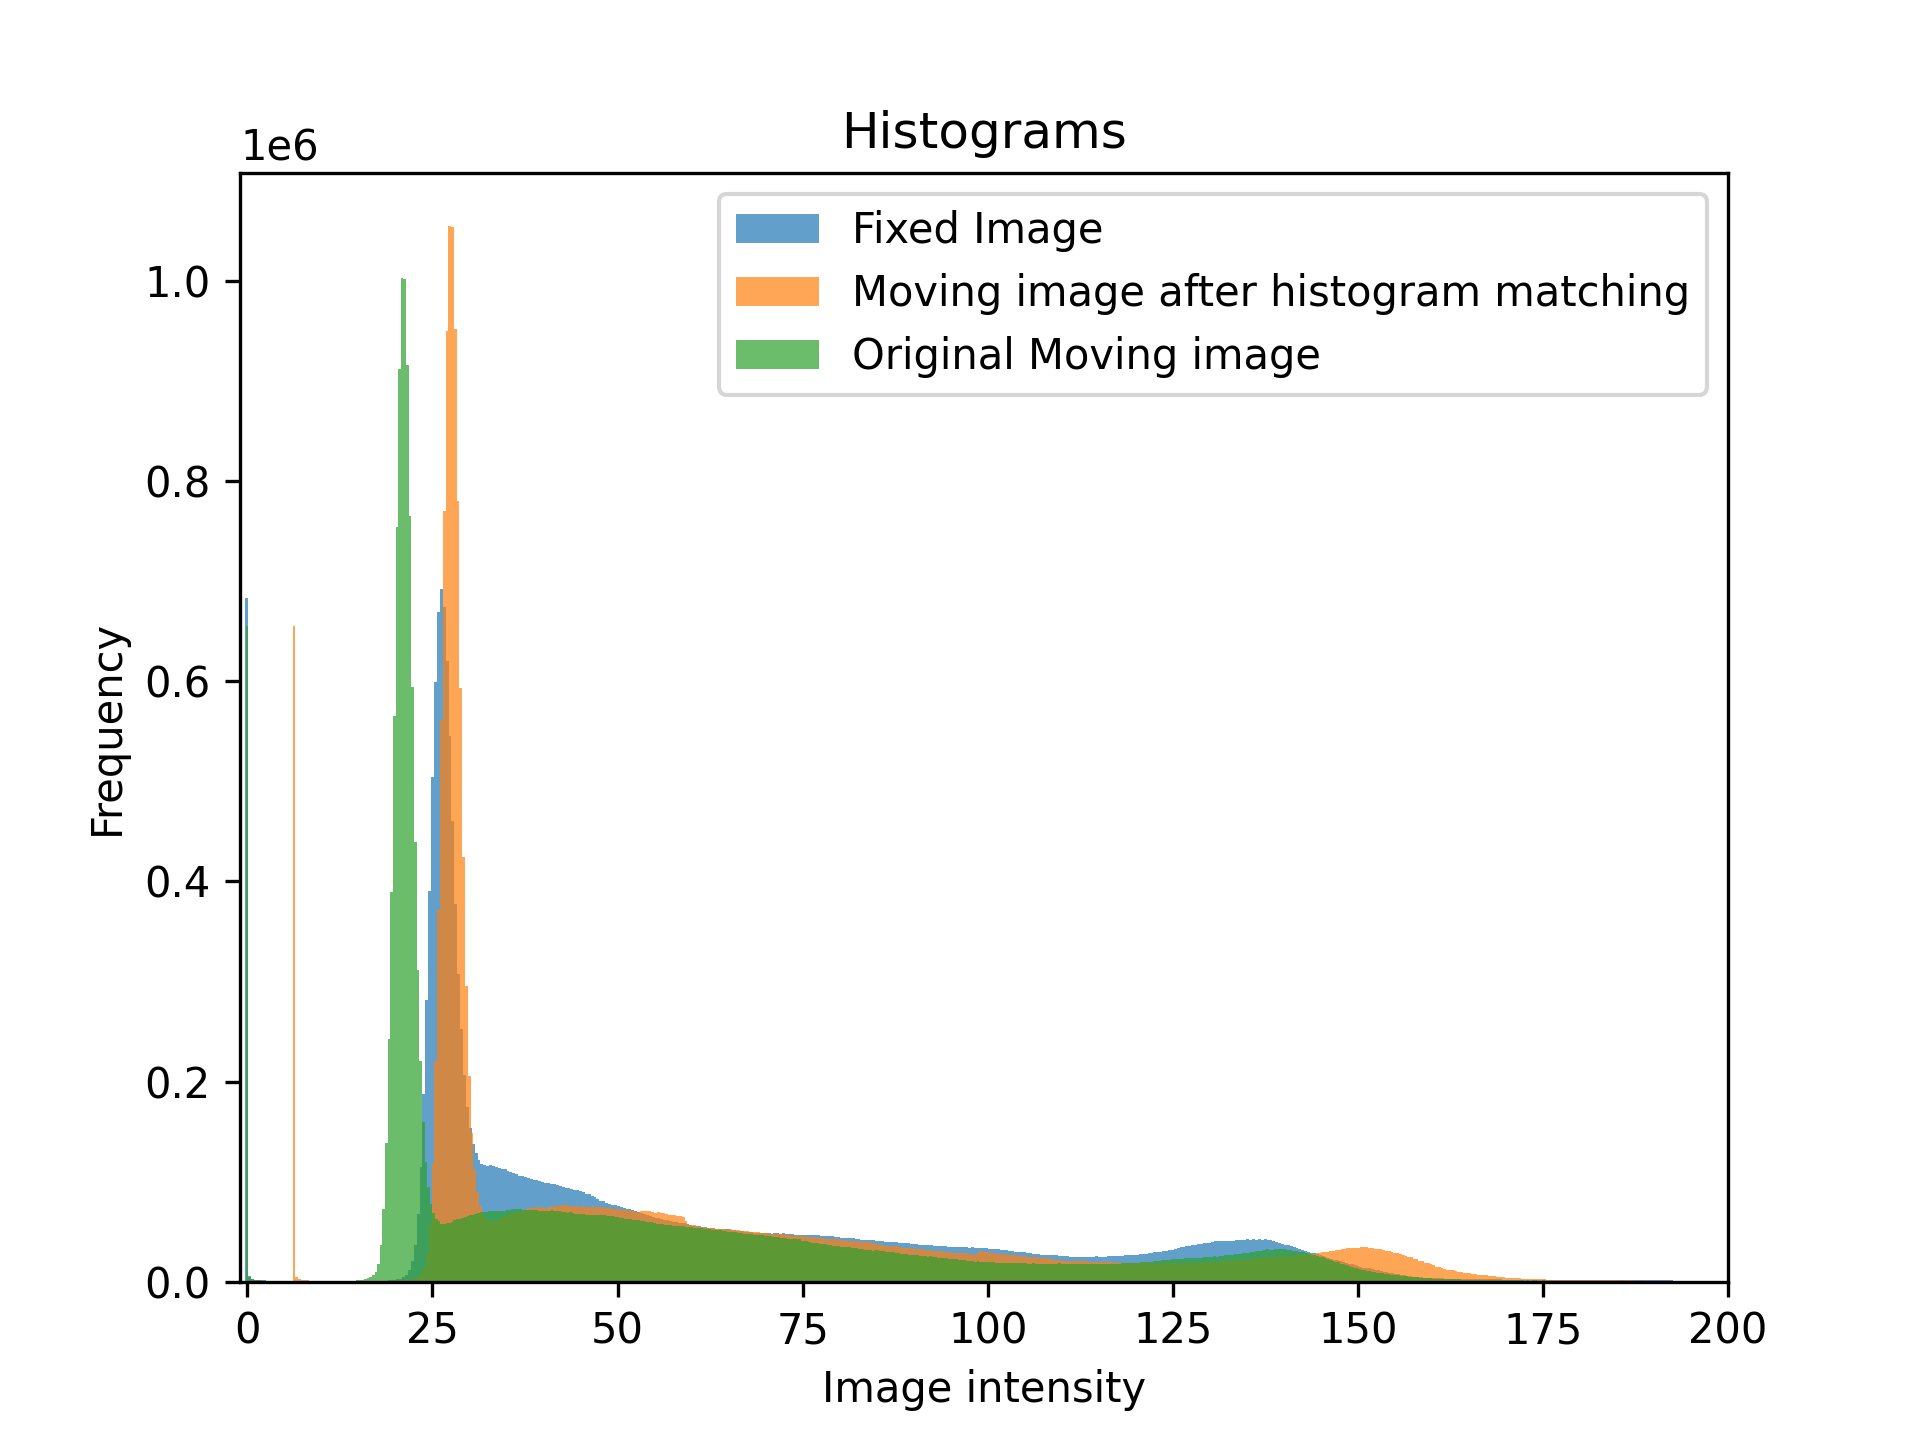
\includegraphics[width=\linewidth]{histogram_plot.png}
    \caption{Ιστογράμματα σταθερής απεικόνισης και κινούμενης πριν και μετά την
             αντιστοίχιση}
    \end{subfigure}

    \label{fig:histogram_matching:1}
\end{figure}
\end{frame}


\subsection{Καταχώρηση απεικονίσεων}


\begin{frame}
\frametitle{Καταχώρηση απεικονίσεων}
\framesubtitle{Αγχίγραμμος μετασχηματισμός (Affine transform)}

Ο αγχίγραμμος μετασχηματισμός έχει 12 βαθμούς ελευθερίας στις 3 διαστάσεις.

\begin{equation*}
    T(x) = A(x - c) + t + c
\end{equation*}

$t$ είναι το διάνυσμα μετατόπισης, $\bm{c}$ το κέντρο περιστροφής και $A$
πίνακας που πραγματοποιεί την περιστροφή, αλλαγή κλίμακας και στρέβλωση.

\begin{figure}[H]
    \centering
    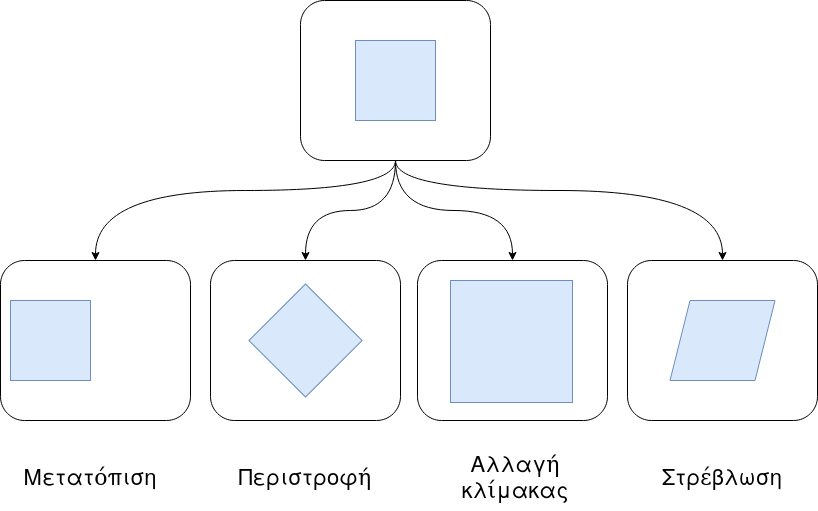
\includegraphics[width=0.4\textwidth]{affine_2}
    \captionsetup{width=0.7\textwidth}
    \caption{Μετατόπιση, περιστροφή, αλλαγή κλίμακας και στρέβλωση ενός
    τετραγώνου.}
\end{figure}

\end{frame}


\begin{frame}
\frametitle{Καταχώρηση απεικονίσεων}
\framesubtitle{Μέση διαφορά τετραγώνων}

Η μέτρηση της ομοιότητας των δύο απεικονίσεων έγινε με την μέση διαφορά
τετραγώνων, με την υπόθεση ότι όμοια βιολογικά σημεία στις απεικονίσεις έχουν
την ίδια φωτεινότητα.

\begin{equation*}
    MSSD(I_F, I_M) = \frac {1} {\abs{\Omega_F}} \sum_{\bm{x_i} \in \Omega_F} 
        \left(\, {I_F\left(\bm{x_i}\right)\, - 
                  I_M\left(\bm{T}\left(\bm{x_i}\right)\,\right)\,}
        \right)^2\, 
\end{equation*}

$I_F$ η σταθερή εικόνα, $I_M$ η κινούμενη εικόνα, $\bm{T}$ ο μετασχηματισμός,
$\Omega_F \subset \R^D \mapsto \R$ το πεδίο ορισμού της σταθερής εικόνα και
$\abs{\Omega_F}$ ο αριθμός την εικονοστοιχείων της σταθερής εικόνας.


\end{frame}


\begin{frame}
\frametitle{Καταχώρηση απεικονίσεων}
\framesubtitle{Χώρος κλίμακας Gauss (Gaussian scale-space) (1/2)}

Ιεραρχική διαδικασία κατά την οποία η πληροφορία των απεικονίσεων αυξάνεται
από τα αρχικά προς τα τελικά στάδια της καταχώρησης, ώστε να υπάρχουν λιγότερες
πιθανότητες να καταλήξει σε κάποιο τοπικό ελάχιστο. Χρησιμοποιεί τον πυρήνα του
Gauss ώστε να μειώσει την πληροφορία.

% Ο πυρήνας του Gauss $g$ και ο τύπος της επιλογής της τυπικής απόκλισης $\sigma$
% ορίζονται ως:

Η τυπική απόκλισης του πυρήνα του Gauss όριζεται από τον τύπο:

\begin{equation*}
    % g(x,y,z,t) = \frac{1} {2 \pi t} e^{\frac{-(x^2 + y^2 + z^2) }{t}}
    % \text{ , }
    \sigma = \frac {f} {2} s
\end{equation*}

Όπου $f$ αναπαριστά το επίπεδο μείωσης της πληροφορίας και έχει τιμές για κάθε
στάδιο $8,4,2,1$ αντίστοιχα. $s$ είναι η απόσταση των εικονοστοιχείων της
απεικόνισης για κάθε διάσταση.


\end{frame}


\begin{frame}
\frametitle{Καταχώρηση απεικονίσεων}
\framesubtitle{Χώρος κλίμακας Gauss (Gaussian scale-space) (2/2)}

\begin{figure}[H]
    \centering

    \begin{subfigure}[b]{0.3\linewidth}
    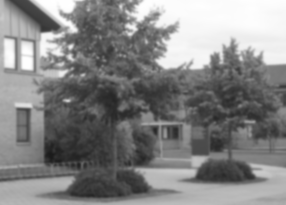
\includegraphics[width=\linewidth]{Scalespace1.png}
    \caption{$\sigma=1$}
    \end{subfigure}
    \begin{subfigure}[b]{0.3\linewidth}
    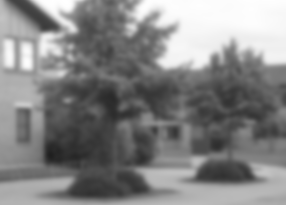
\includegraphics[width=\linewidth]{Scalespace2.png}
    \caption{$\sigma=2$}
    \end{subfigure}

    \begin{subfigure}[b]{0.3\linewidth}
    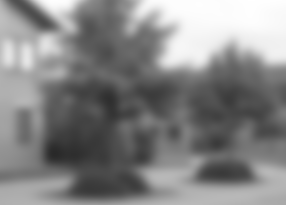
\includegraphics[width=\linewidth]{Scalespace3.png}
    \caption{$\sigma=4$}
    \end{subfigure}
    \begin{subfigure}[b]{0.3\linewidth}
    
\includegraphics[width=\linewidth]{Scalespace4.png}
    \caption{$\sigma=8$}
    \end{subfigure}

    \caption{Χώρος κλίμακας Gauss για διάφορες τιμές της τυπικής απόκλισης.}
    \label{fig:tGauss}
\end{figure}


\end{frame}


\begin{frame}
\frametitle{Καταχώρηση απεικονίσεων}
\framesubtitle{Λοιπές επιλογές}

\begin{itemize}
    \item<1-> Ο Αλγόριθμος βελτιστοποίησης που χρησιμοποιήθηκαι είναι ο
        αλγόριθμος προσαρμοστικής στοχαστικής απότομης καθόδου (Adaptive
        Stochastic Gradient Descent, ASGD).
    \item<2-> Η παρεμβολή των σημείων των απεικονίσεων έγινε με γραμμική
        παρεμβολή.
    \item<3-> Χρησιμοποιήθηκε δειγματοληψία $80\%$ του συνολικού αριθμού των
        εικονοστοιχείων μίας απεικόνισης για να μειωθεί ο χρόνο υπολογισμού που
        απαιτείται για την καταχώρηση.
    \item<4-> Χρησιμοποιήθηκε μάσκα για την κινούμενη εικόνα. Η μάσκα αυτή
        αποτελείται από όλα τα εικονοστοιχεία της απεικόνισης που δεν ανήκουν
        στο παρασκήνιο. Με αυτόν τον τρόπο συνεισφέρουν μόνο τα εικονοστοιχεία
        των απεικονίσεων που ανήκουν σε βιολογικές ομάδες που πρόκειται να
        κατανεμηθούν.
\end{itemize}

\end{frame}



\begin{frame}
\frametitle{Καταχώρηση απεικονίσεων}
\framesubtitle{Αποτέλεσμα καταχώρησης}

\begin{figure}[H]
    \centering

    \begin{subfigure}[t]{0.24\linewidth}
    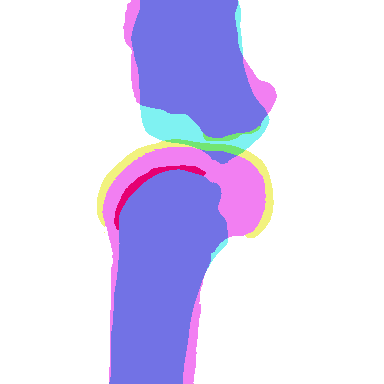
\includegraphics[width=\linewidth]{combination_label_before_registration_1.png}
    \caption{Πριν}
    \end{subfigure}
    \begin{subfigure}[t]{0.24\linewidth}
    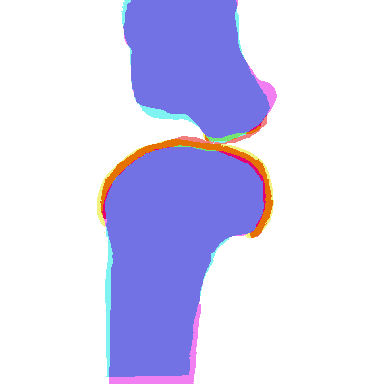
\includegraphics[width=\linewidth]{combination_label_after_registration_1.png}
    \caption{Μετά}
    \end{subfigure}
    \begin{subfigure}[t]{0.24\linewidth}
    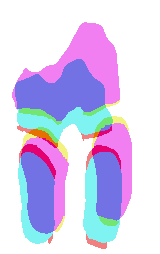
\includegraphics[width=\linewidth]{combination_label_before_registration_2.png}
    \caption{Πριν}
    \end{subfigure}
    \begin{subfigure}[t]{0.24\linewidth}
    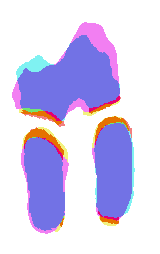
\includegraphics[width=\linewidth]{combination_label_after_registration_2.png}
    \caption{Μετά}
    \end{subfigure}

    \caption{Τομή απεικονίσεων σταθερής και κινούμενης απεικόνισης πριν και μετά
             την καταχώρηση.} 
\end{figure}

\end{frame}


\subsection{Επιλογή ατλάντων}



\begin{frame}
\frametitle{Επιλογή ατλάντων}

Μετρική για την επιλογή αυτή χρησιμοποιείται η μέση διαφορά τετραγώνων των
εικονοστοιχείων των απεικονίσεων που δεν ανήκουν στο παρασκήνιο. Επιλέγονται οι
$N$ άτλαντες με τη μικρότερη τιμή.

\begin{equation*}
    mse_i = \frac {1} {\abs{p_i}} \sum_{\bm{x} \in p_i} ( I(\bm{x}) -
                I_i(\bm{x})  )^2
    \text{ ,όπου }
    p_i = \{\bm{x}| \bm{x} \in L_i, L_i > 0 \}
\end{equation*}

$I$ είναι η σταθερή απεικόνιση, $I_i$ και $L_i$ μία κινούμενη απεικόνιση και οι
ετικέτες της αντίστοιχα για τον $i$-οστό άτλαντα. Επίσης, $\abs{p_i}$ είναι ο
αριθμός των στοιχείων που χρησιμοποιούνται για τον υπολογισμό της μετρικής.

\end{frame}


\subsection{Μέθοδος 1: Αραιή μέθοδος βασισμένη σε τμήματα (Sparse Patch-Based
Method, SPBM)}



\begin{frame}
\frametitle{Μέθοδος 1: Αραιή μέθοδος βασισμένη σε τμήματα \\
(Sparse Patch-Based Method, SPBM)}

\begin{figure}[H]
    \centering
    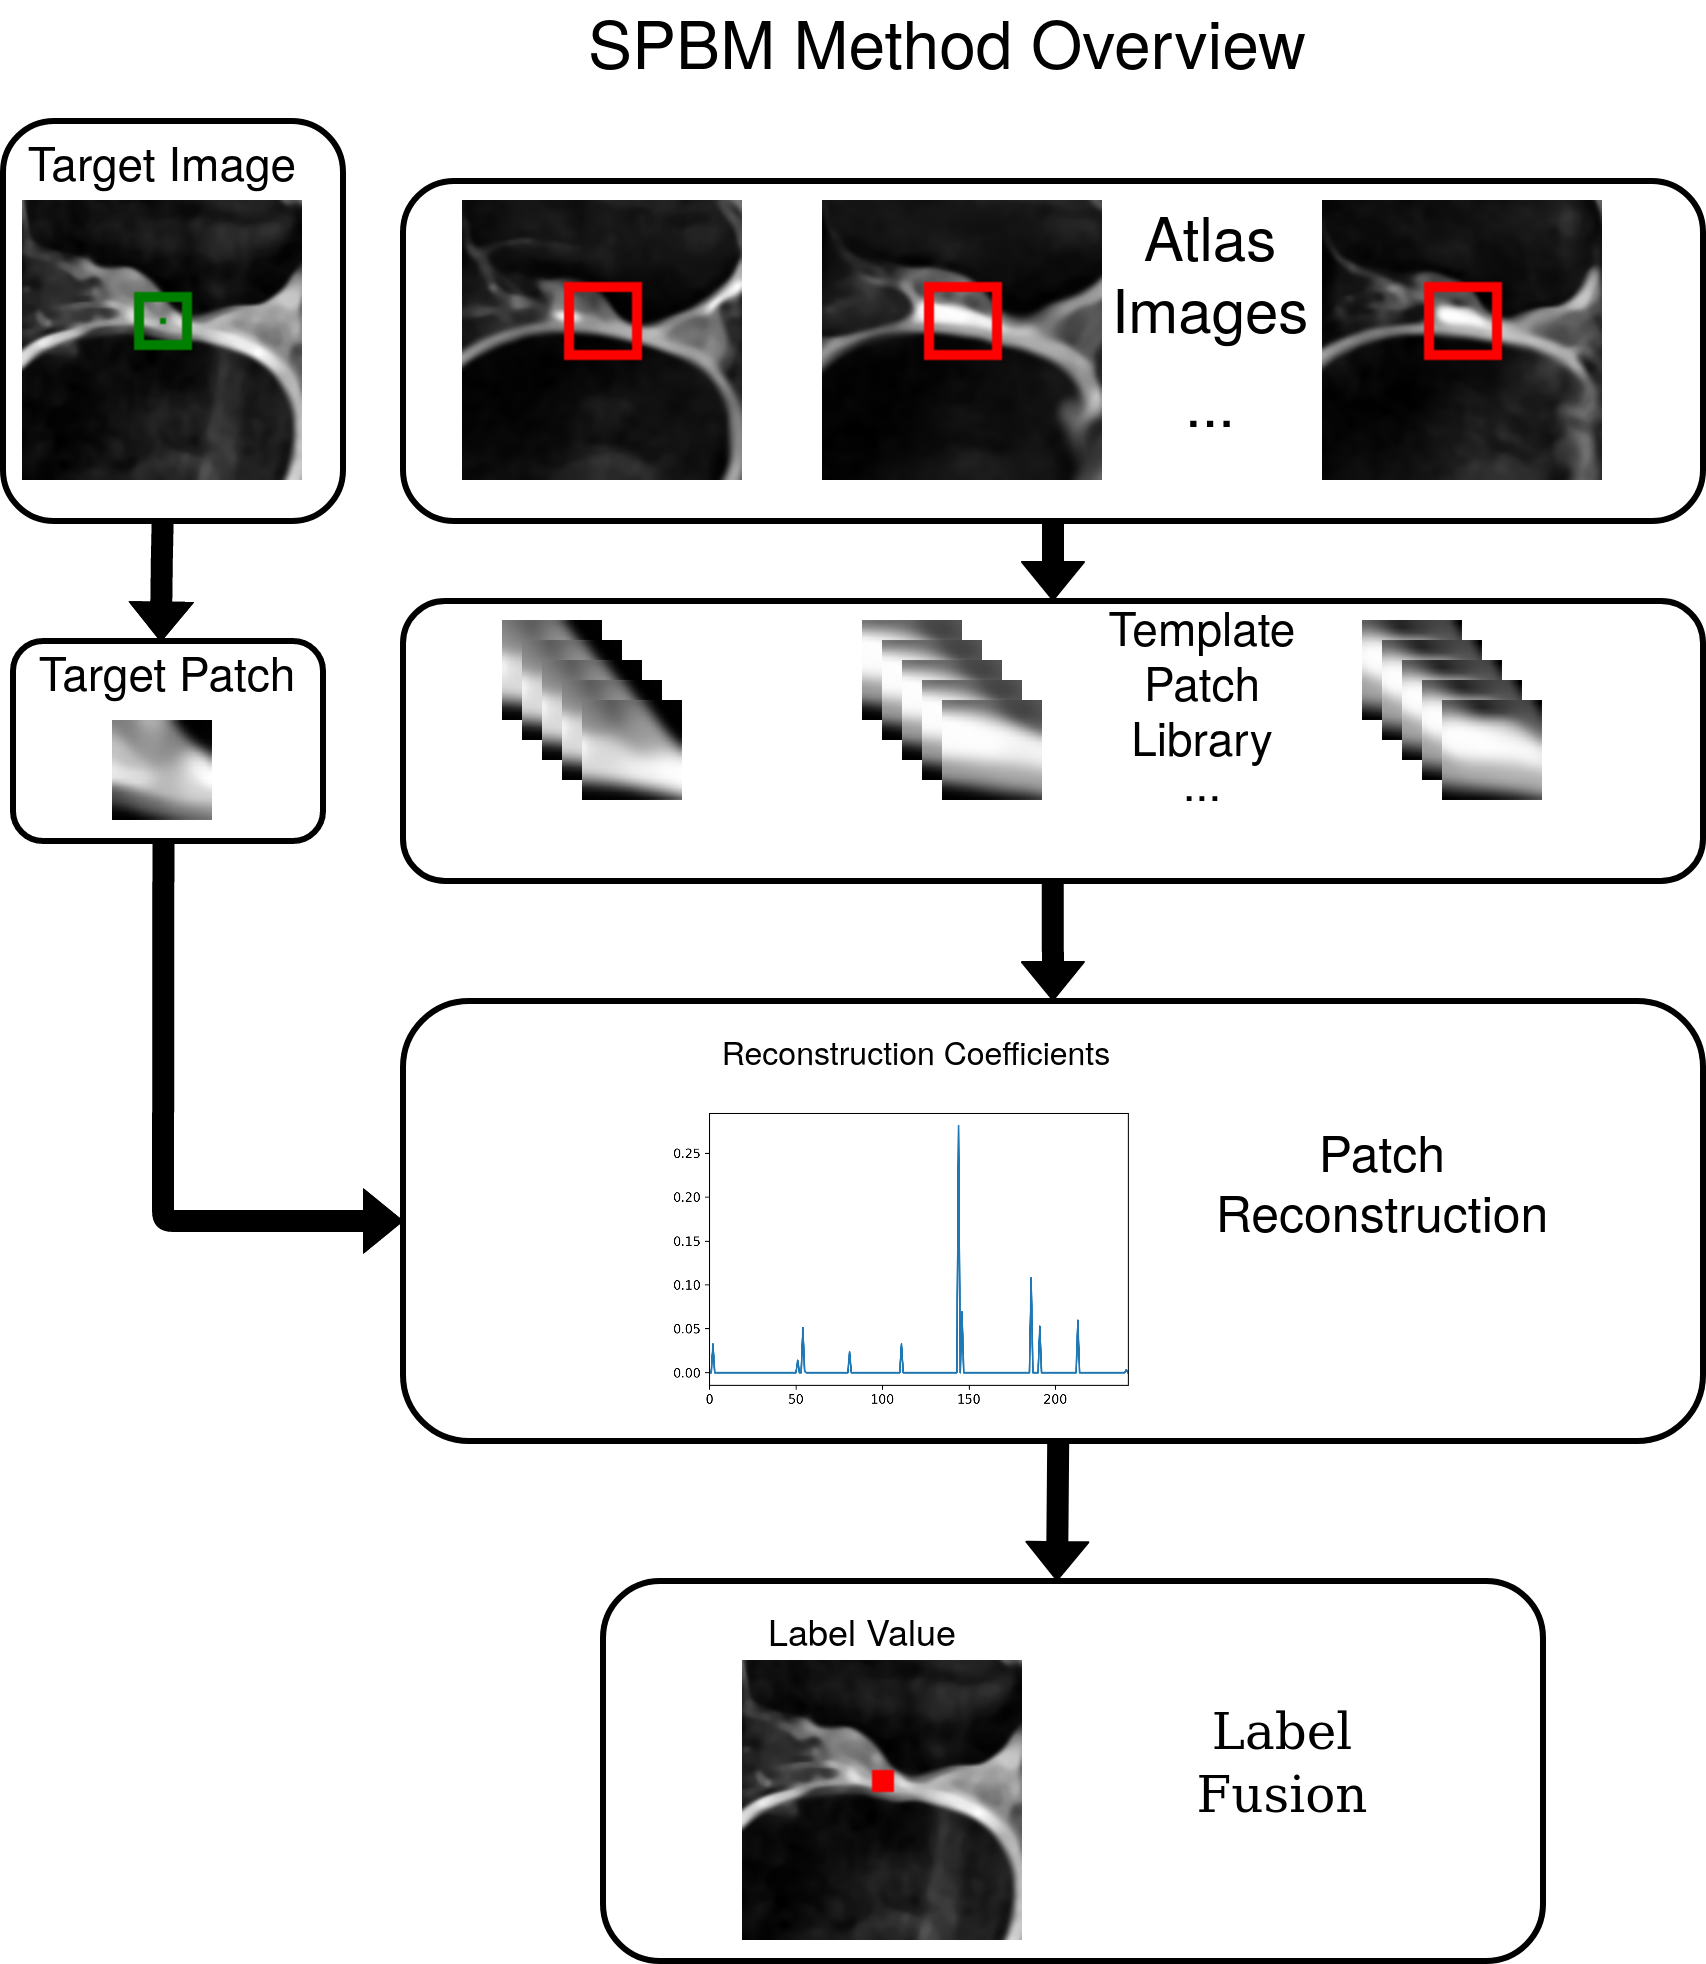
\includegraphics[height=0.8\textheight]{SPBM_method.png}
    \caption{Διάγραμμα ροής της αραιής μεθόδου βασισμένης σε τμήματα (SPBM).}
    \label{fig:SPBM_method:1}
\end{figure}

\end{frame}


\begin{frame}
\frametitle{Μέθοδος 1: Αραιή μέθοδος βασισμένη σε τμήματα \\
(Sparse Patch-Based Method, SPBM)}

Οι συντελεστές ανοικοδοόμησης $w_i(\bm{x},\bm{y})$ υπολογίζονται από τη
συνάρτηση:

\begin{equation*}
    \argminB_{\{w_i(\bm{x},\bm{y})\}} { \frac{1} {2} \norm {\sum_{i=1}^{n}
    \sum_{\bm{y} \in N_i(\bm{x})} A_{\bm{y}}^i w_i(\bm{x},\bm{y}) -
    b_{\bm{x}}}_2^2 }
    + \lambda \sum_{i=1}^{n} \sum_{\bm{y} \in N_i(\bm{x})}
    \abs{w_i(\bm{x},\bm{y})}
\end{equation*}

Για κάθε ετικέτα εκτός του παρασκηνίου υπολογίζεται η εξίσωση του πλαισίου
συγχώνευσης κατηγοριών, για να παραχθεί η ετικέτα $L(\bm{x})$ για το
εικονοστοιχείο $\bm{x}$.

\begin{equation*}
    L(\bm{x})=\frac{ \sum_{i=1}^{n}  \sum_{\bm{y}\in\Omega}
                     w_i(\bm{x},\bm{y})L_i(\bm{y})}
    { \sum_{i=1}^{n}  \sum_{\bm{y}\in\Omega} w_i(\bm{x},\bm{y}) }
    , \forall \bm{x}\in\Omega
\end{equation*}

Η τελική ετικέτα επιλέγεται για το $L(\bm{x}) \geq 0.5$ αν υπάρχει αλλίως,
επιλέγεται η ετικέτα του παρασκηνίου.

\end{frame}


\subsection{Μέθοδος 2: Ταξινόμηση αραιής αναπαράστασης (Sparse Representation
Classification, SRC)}


\begin{frame}
\frametitle{Μέθοδος 2: Ταξινόμηση αραιής αναπαράστασης \\
(Sparse Representation Classification, SRC)}

\begin{figure}[H]
    \centering
    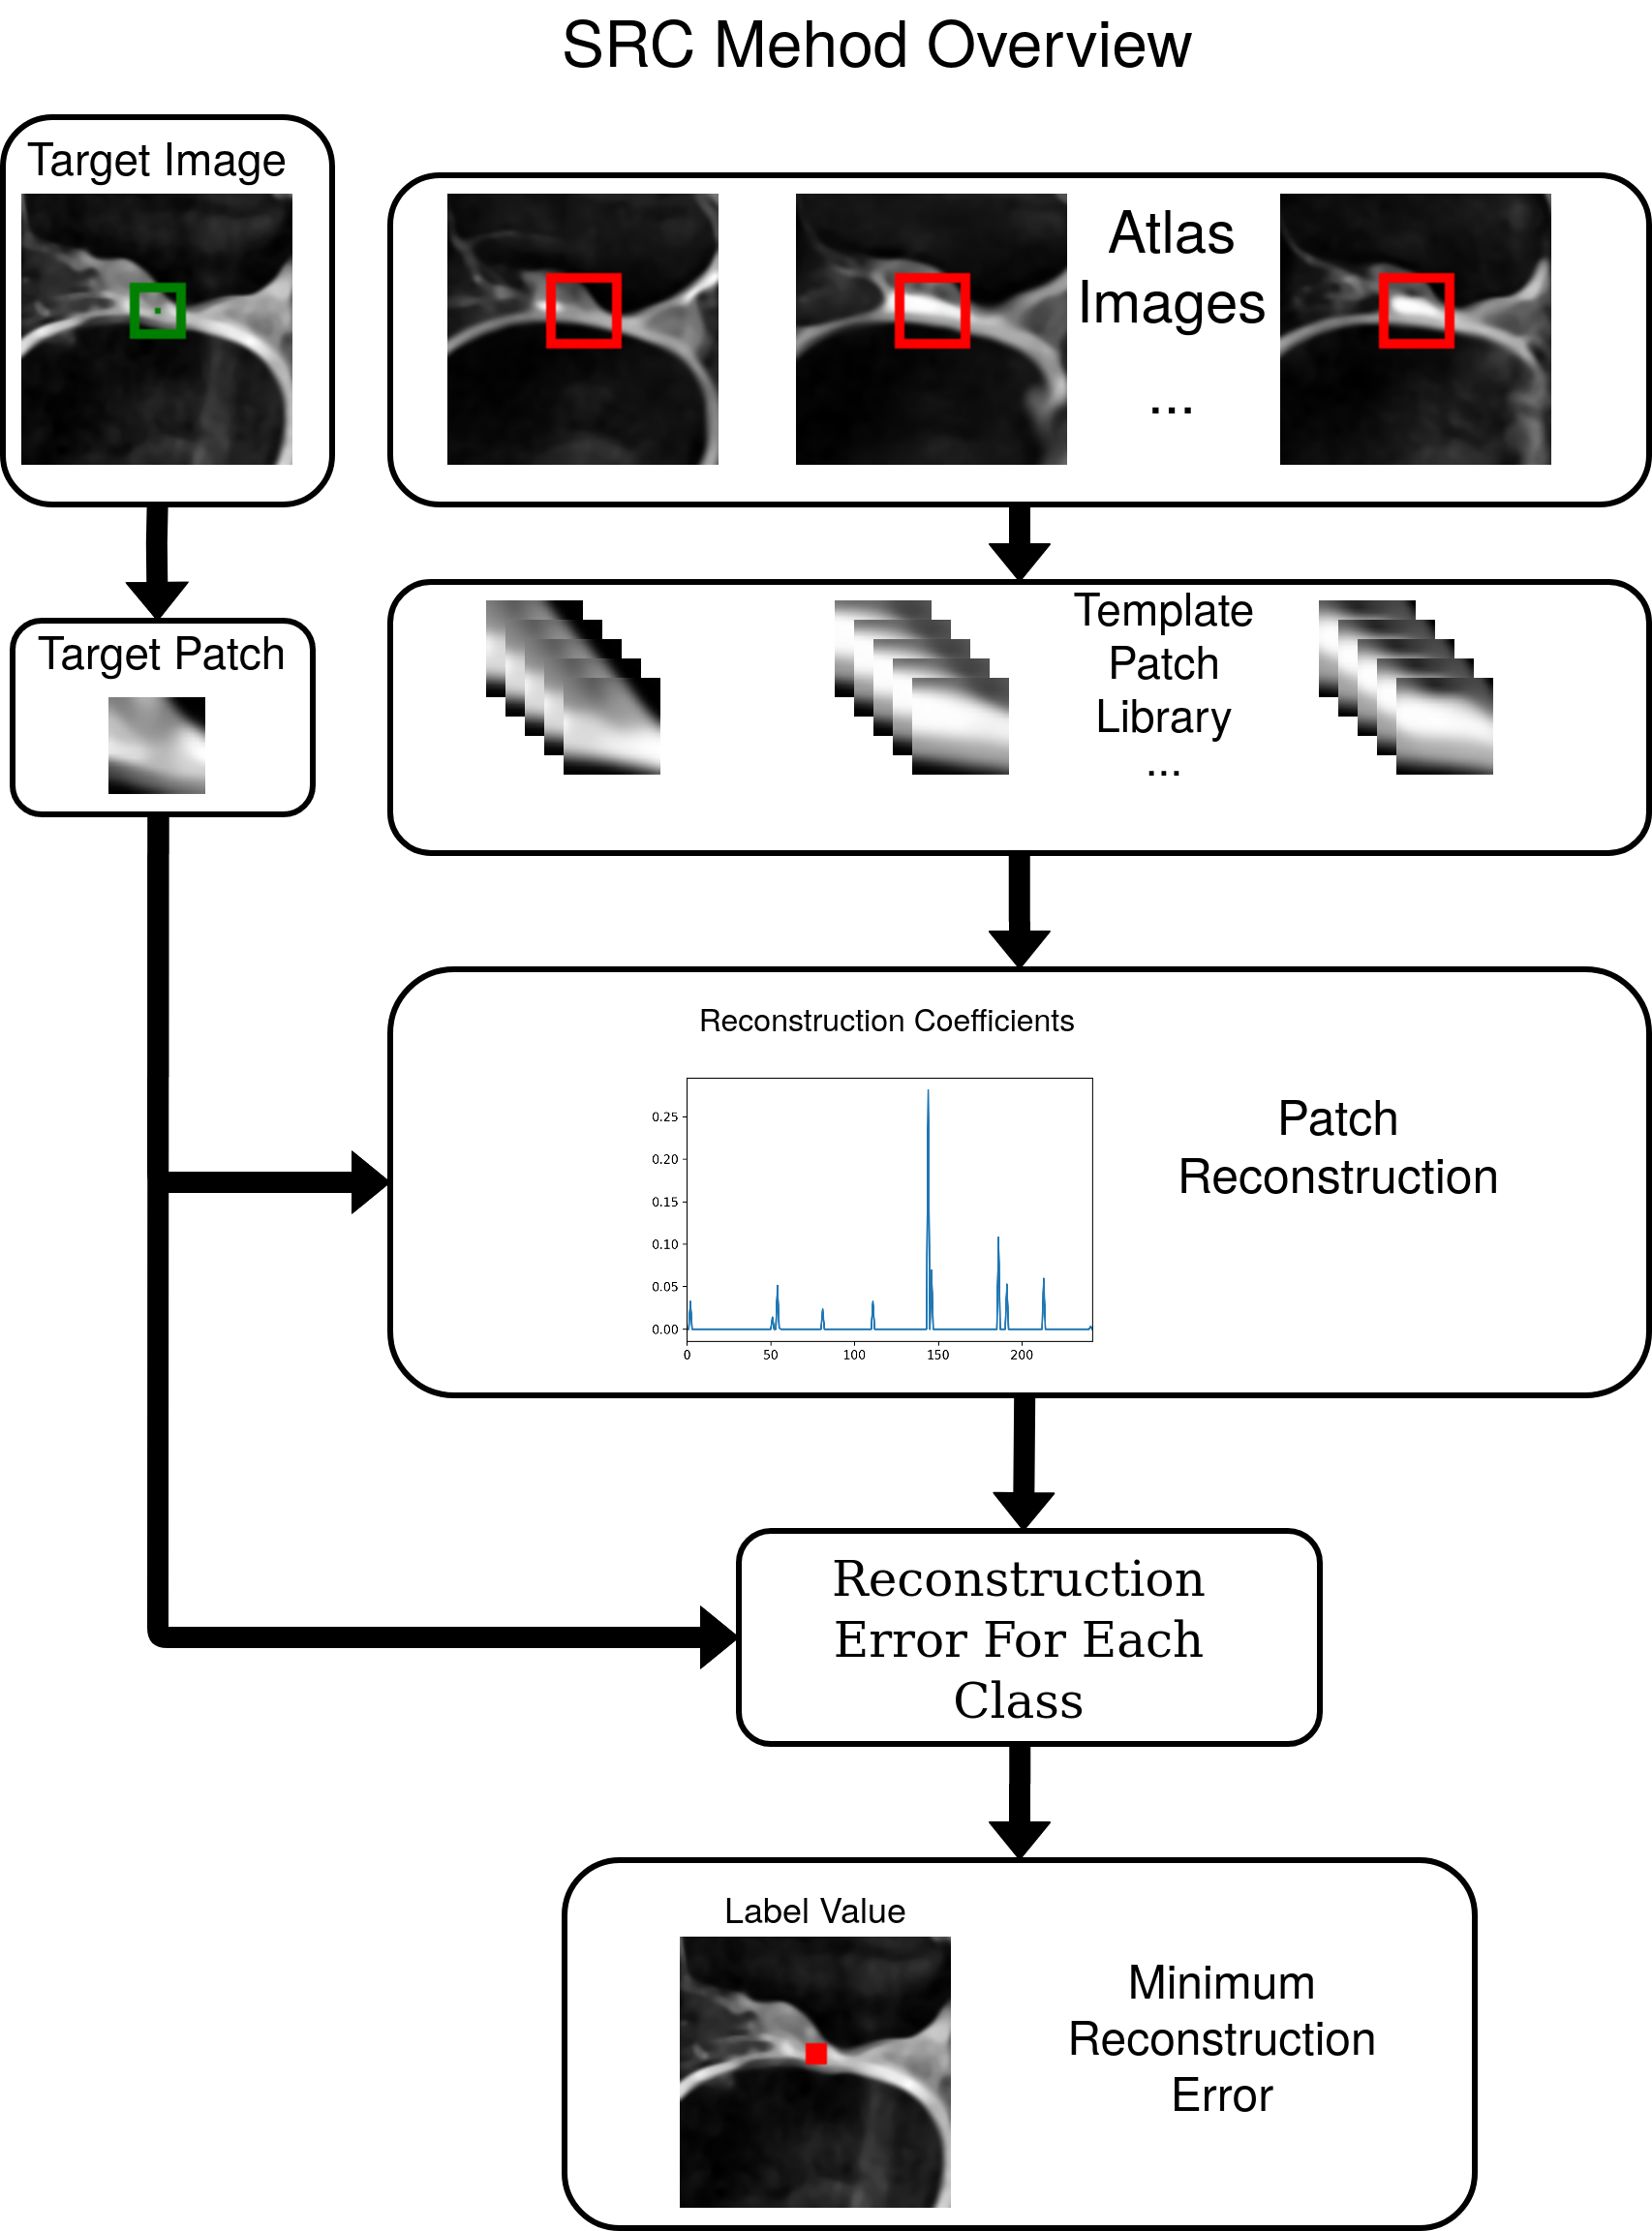
\includegraphics[height=0.8\textheight]{SRC_method.png}
    \caption{Διάγραμμα ροής της μεθόδου ταξινόμησης αραιής αναπαράστασης (SRC).}
\end{figure}

\end{frame}

\begin{frame}
\frametitle{Μέθοδος 2: Ταξινόμηση αραιής αναπαράστασης \\
(Sparse Representation Classification, SRC)}

Οι συντελεστές ανοικοδοόμησης $w_{\bm{x}}$ υπολογίζονται από τη συνάρτηση:

\begin{equation*}
    \argminB_{w_{\bm{x}}} { \frac{1} {2} \norm { A w_{\bm{x}} - b_{\bm{x}} }_2^2
              + \lambda \norm{w_{\bm{x}}}_1 }
\end{equation*}

Το σφάλμα ανοικοδόμησης για κάθε ετικέτα $j = 0,...,C$ ορίζεται ως:

\begin{equation*} 
    r_j(b_{\bm{x}}) = \norm{ b_{\bm{x}} - A^j w_{\bm{x}}^j }
\end{equation*}

Τέλος, η τελική ετικέτα $v$ του εικονοστοιχείου προς ταξινόμηση ορίζεται ως:

\begin{equation*} 
    v = \argminB_{j} { \left( r_j(b_{\bm{x}}) \right) } \text{ , } j = 0,...,C
\end{equation*}

\end{frame}

 
\subsection{Μέθοδος 3: Κατάτμηση βασισμένη σε τμήματα με τη χρήση πληροφορίας
από ειδικούς (Patch-Based Segmentation using Expert Priors, PBSEP)}


\begin{frame}
\frametitle{\normalsize Μέθοδος 3: Κατάτμηση βασισμένη σε τμήματα με τη χρήση
πληροφο-\\ρίας από ειδικούς (Patch-Based Segmentation using Expert Priors, PBSEP)}

\begin{figure}[H]
    \centering
    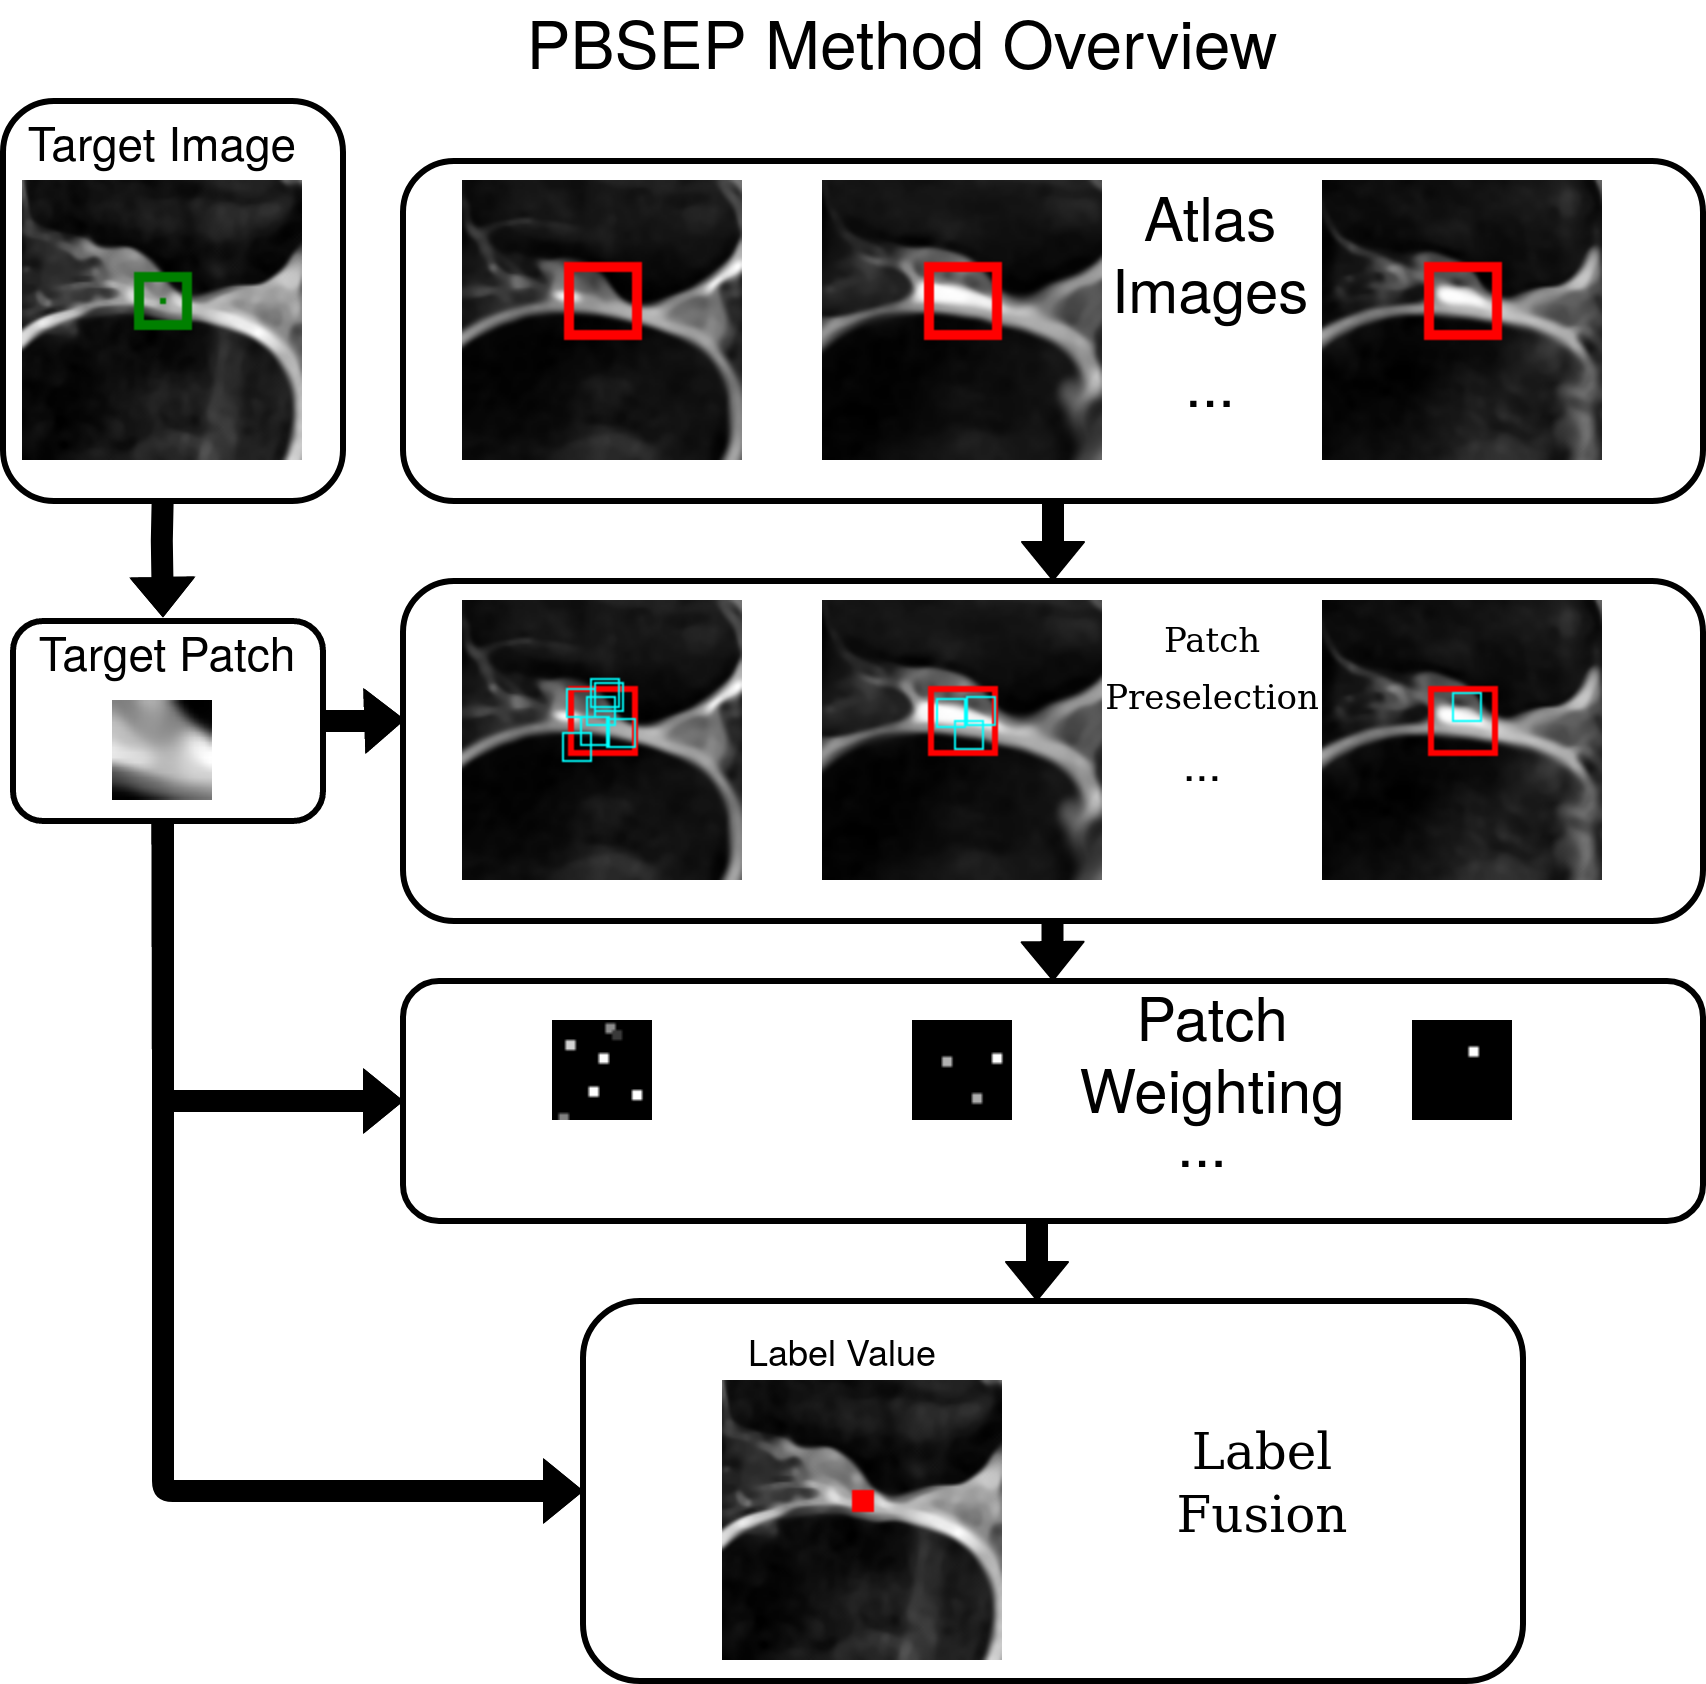
\includegraphics[height=0.8\textheight]{PBSEP_method.png}
    \caption{Διάγραμμα ροής της κατάτμησης βασισμένης σε τμήματα με τη χρήση
             πληροφορίας από ειδικούς (PBSEP).}
\end{figure}

\end{frame}


\begin{frame}
\frametitle{\normalsize Μέθοδος 3: Κατάτμηση βασισμένη σε τμήματα με τη χρήση
πληροφο-\\ρίας από ειδικούς (Patch-Based Segmentation using Expert Priors, PBSEP)}

Η επιλογή των patches και η μετρική ομοιότητας ορίζονται από την εξίσωση:

\begin{equation*}
    w(x_i, x_{s,j}) = 
    \begin{cases}
        exp\left( \frac {- \norm{P(x_i) - P(x_{s,j})}_2^2 } {h} \right)
            & \text{if } ss > th\\
        0   & \text{otherwise}
    \end{cases}
\end{equation*}

Όπου $P(x)$ είναι το patch γύρο από το εικονοστοιχείο $x$. Η σταθερά $th = 0.95$
και οι συναρτήσεις:

\begin{equation*}
    ss = \frac {2 \mu_i \mu_{s,j}} {\mu_i^2 + \mu_{s,j}^2} 
         \frac {2 \sigma_i \sigma_{s,j}} {\sigma_i^2 + \sigma_{s,j}^2}
    % \text{ , }
\end{equation*}
\begin{equation*}
    h = \argminB_{x_{x,j}} \norm{P(x_i) - P(x_{s,j})}_2 + \epsilon
\end{equation*}

\end{frame}


\begin{frame}
\frametitle{\normalsize Μέθοδος 3: Κατάτμηση βασισμένη σε τμήματα με τη χρήση
πληροφο-\\ρίας από ειδικούς (Patch-Based Segmentation using Expert Priors, PBSEP)}

Για κάθε ετικέτα εκτός του παρασκηνίου υπολογίζεται η εξίσωση του πλαισίου
συγχώνευσης κατηγοριών, για να παραχθεί η ετικέτα $L(\bm{x})$ για το
εικονοστοιχείο $\bm{x}$.

\begin{equation*}
    L(\bm{x})=\frac{ \sum_{i=1}^{n}  \sum_{\bm{y}\in\Omega}
                     w_i(\bm{x},\bm{y})L_i(\bm{y})}
    { \sum_{i=1}^{n}  \sum_{\bm{y}\in\Omega} w_i(\bm{x},\bm{y}) }
    , \forall \bm{x}\in\Omega
\end{equation*}

Η τελική ετικέτα επιλέγεται για το $L(\bm{x}) \geq 0.5$ αν υπάρχει αλλίως,
επιλέγεται η ετικέτα του παρασκηνίου.

\end{frame}


\section{Πειράματα και αποτελέσματα}
\subsection{Δεδομένα}

\begin{frame}
\frametitle{Δεδομένα}

Τα δεδομένα που χρησιμοποιήθηκαν προέρχονται από το Osteoarthritis Initiative
Zuse Institute Berlin (OAI ZIB).Οι κλάσεις της κατάτμησης που χρησιμοποιήθηκαν
αποτελούνται από τα οστά, τους χόνδρους και το παρασκήνιο. Χρησιμοποιήθηκαν 46 από
τα 507 δείγματα που διατίθενται και καλύπτουν όλο το φάσμα του βαθμού
οστεοαρθρίτιδας.

\begin{table}[h!]
    \centering
    \begin{tabular}{|c|c|} 
        \hline
        MRI scanner            & Siemens 3T Trio \\ 
        MRI sequence           & DESS            \\
        Acquisition plane      & Sagittal        \\
        Image resolution in mm & 0.36×0.36×0.7   \\
        Timepoints             & Baseline        \\
        \hline
    \end{tabular}
    \caption{Χαρακτηριστικά δεδομένων OAI ZIB.}
    \label{dataset:1}
\end{table}


\end{frame}


\subsection{Τρόπος αξιολόγησης και σύγκρισης}


\begin{frame}
\frametitle{Τρόπος αξιολόγησης και σύγκρισης}

Ως μετρική του αποτελέσματος χρησιμοποιείται ο συντελεστής ομοιότητας Dice: 

\begin{equation*}
    DSC = \frac{2 \abs{X \cap Y}} {\abs{X} + \abs{Y}}
\end{equation*}

Επίσης, για κάθε πείραμα χρησιμοποιήθηκε η διασταυρωμένη επικύρωση αφήνω ένα έξω
(leave-one-out cross-validation).  

\begin{figure}[H]
    \centering
    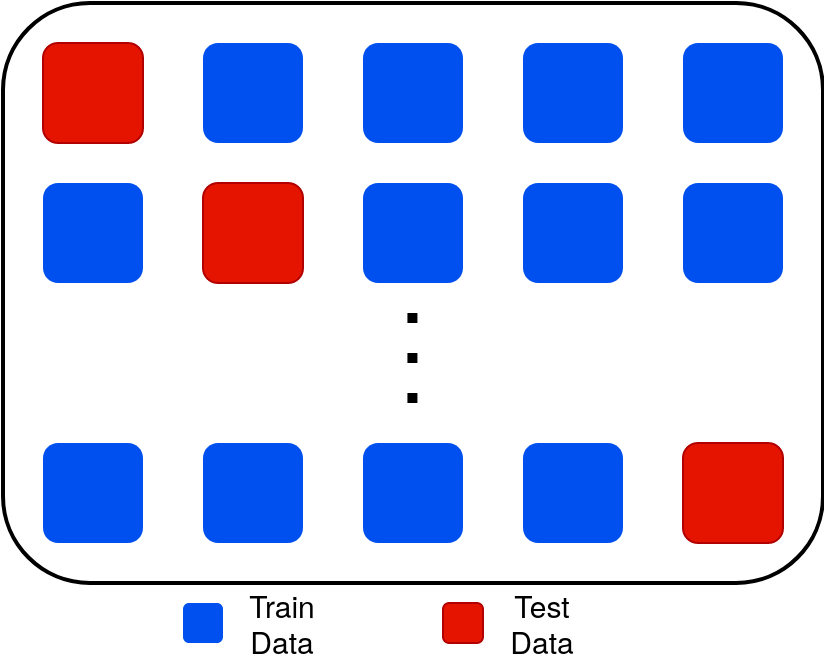
\includegraphics[height=0.4\textheight]{leave_one_out}
    \caption{Διαδικασία διασταυρωμένη επικύρωση αφήνω ένα έξω (leave-one-out
             cross-validation).}
\end{figure}

\end{frame}


\subsection{Επιλογή παραμέτρων}

\begin{frame}
\frametitle{Παράμετροι}
Οι παράμετροι που είναι κοινοί για όλες τις μεθόδους είναι:

\begin{enumerate}
    \item Το μέγεθος της περιοχής αναζήτησης.
    \item Το μέγεθος του patch.
    \item Ο αριθμός των ατλάντων που χρησιμοποιείται στην κατάτμηση.
\end{enumerate}

Ακόμα, η αραιή μέθοδος βασισμένη σε τμήματα (SPBM) και η μέθοδος
ταξινόμησης αραιής αναπαράστασης (SRC) έχουν την παράμετρο $\lambda$ του
ελάχιστα απόλυτου τελεστή συρρίκνωσης και επιλογής (Lasso).
\end{frame}


\begin{frame}
\frametitle{Διασταυρωμένη επικύρωση για την παράμετρο $\lambda$ του τελεστή
Lasso}
\framesubtitle{Μέθοδος 1: Αραιή μέθοδος βασισμένη σε τμήματα (SPBM)}

\begin{figure}[H]
    \centering

    \begin{subfigure}[b]{0.42\linewidth}
    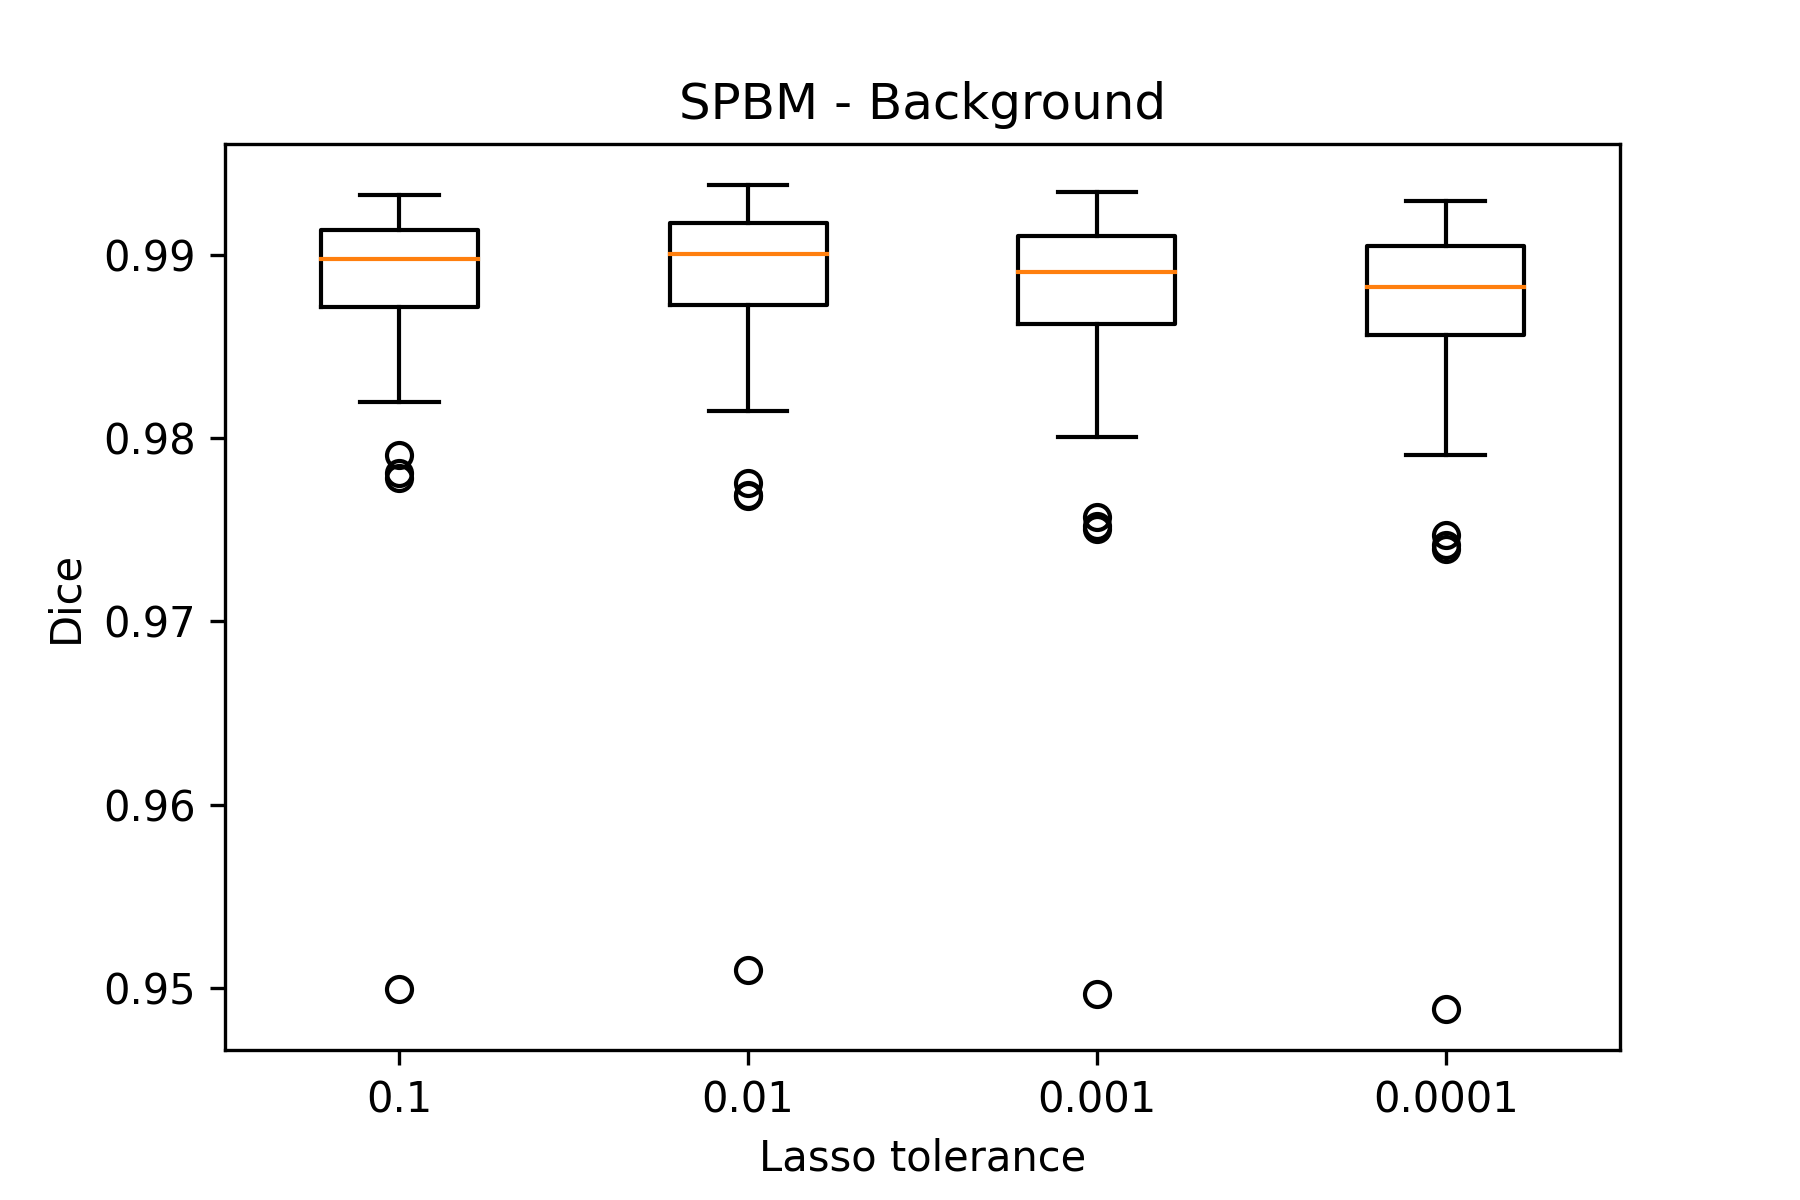
\includegraphics[width=\linewidth]{SPBM_Lasso_tolerance_Background_plot.png}
    \caption{Παρασκήνιο}
    \end{subfigure}
    \begin{subfigure}[b]{0.42\linewidth}
    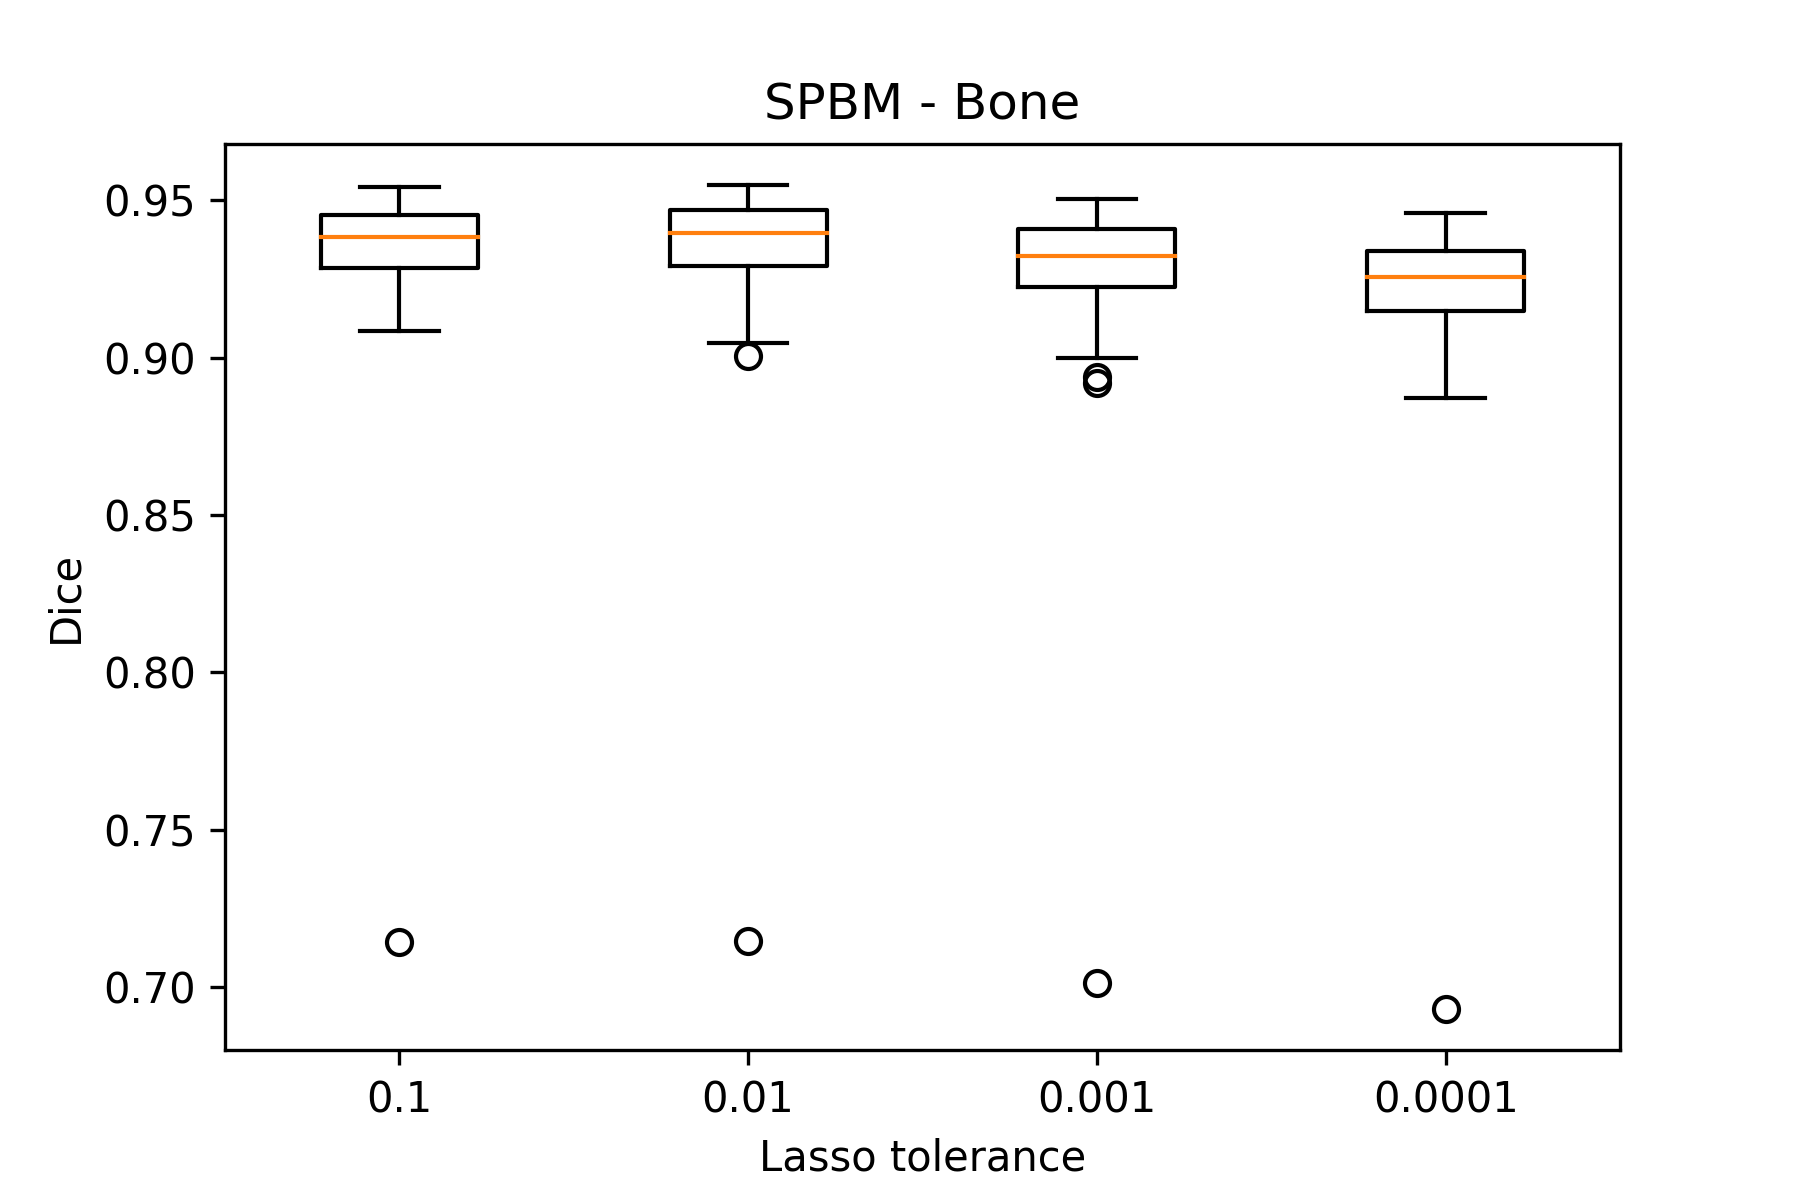
\includegraphics[width=\linewidth]{SPBM_Lasso_tolerance_Bone_plot.png}
    \caption{Οστά}
    \end{subfigure}

    \begin{subfigure}[b]{0.42\linewidth}
    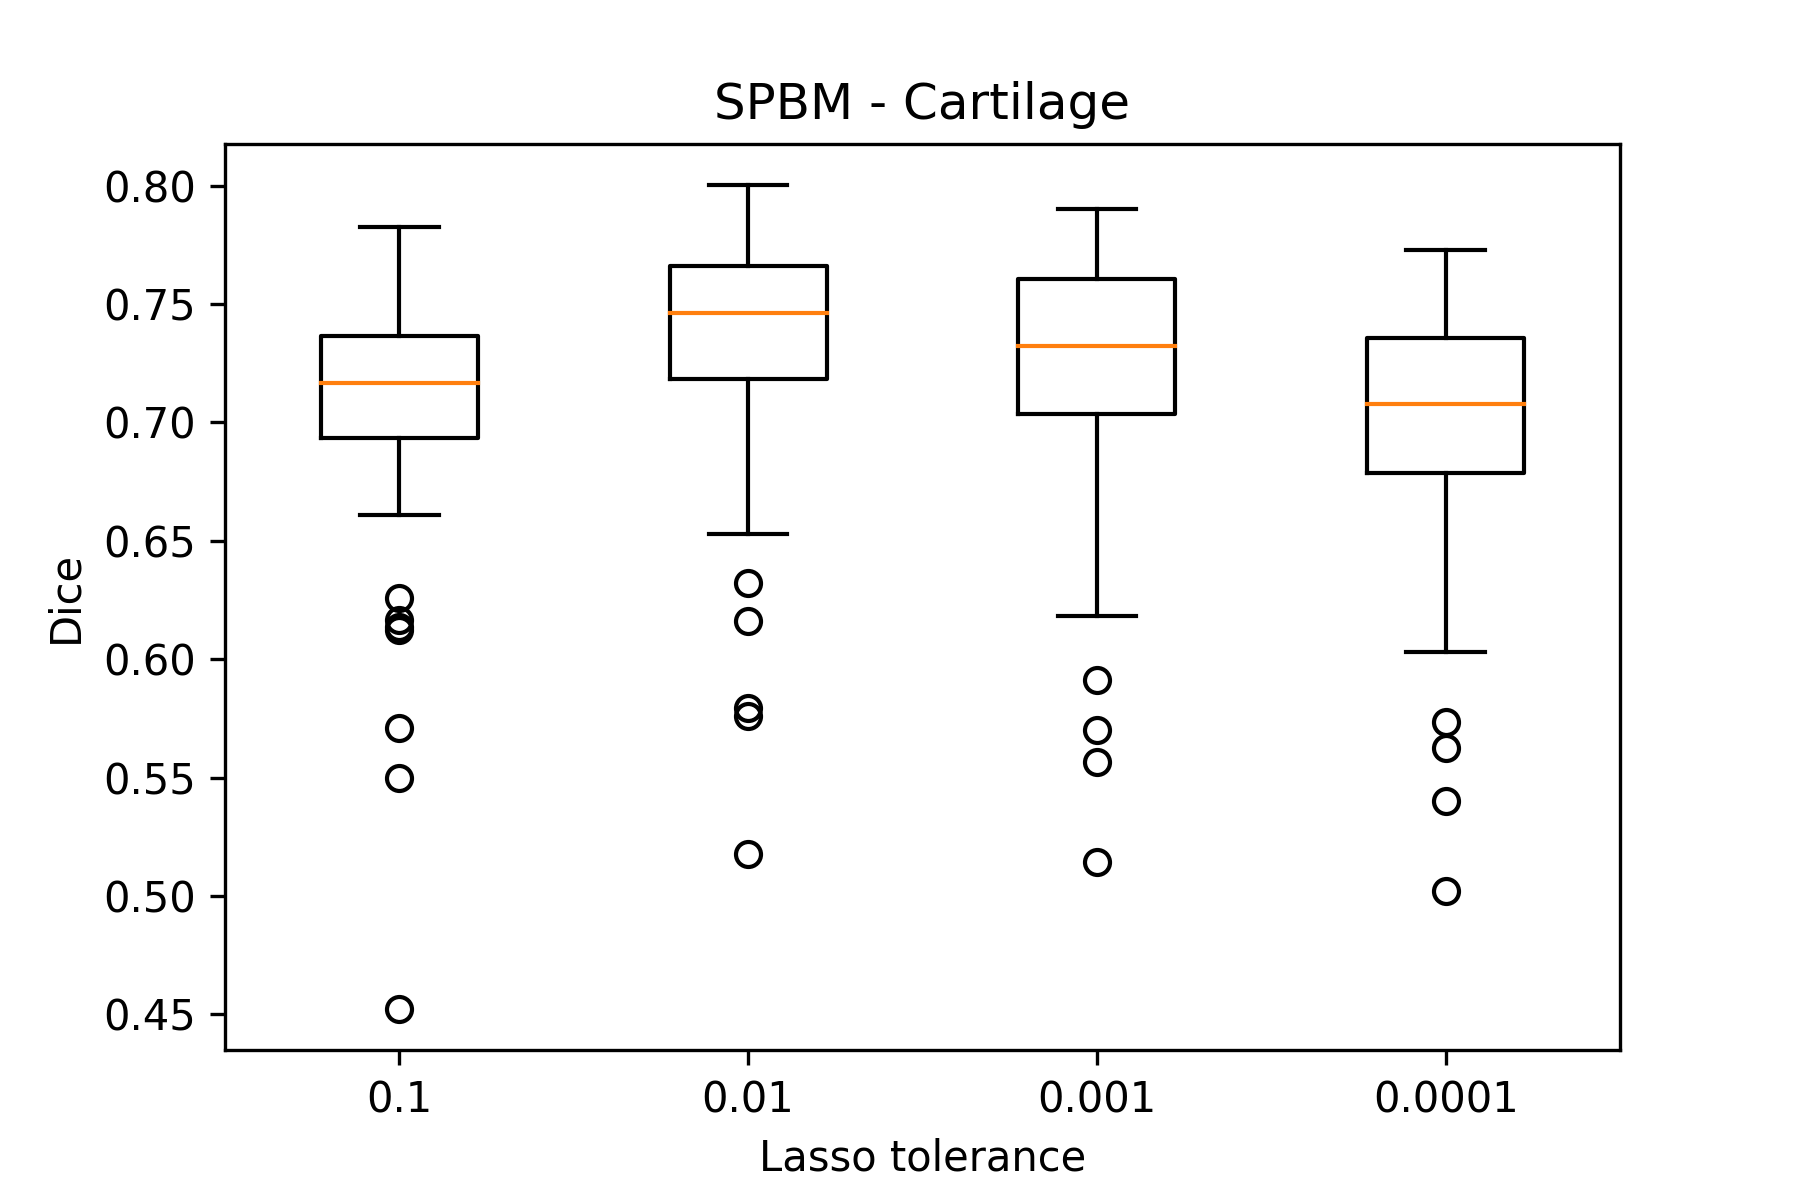
\includegraphics[width=\linewidth]{SPBM_Lasso_tolerance_Cartilage_plot.png}
    \caption{Χόνδροι}
    \end{subfigure}
    \begin{subfigure}[b]{0.42\linewidth}
        \begin{tabular}[t]{|l|c|} 
            \multicolumn{2}{c}{\footnotesize Σταθερές παράμετροι} \\
            \hline
            \footnotesize Αριθμός ατλάντων & \footnotesize  4 \\ 
            \hline
            \footnotesize Μέγεθος περιοχής αναζήτησης & \footnotesize  [5,5,5] \\ 
            \hline
            \footnotesize Μέγεθος patch & \footnotesize [3,3,3] \\
            \hline
            \multicolumn{2}{c}{\footnotesize Επιλογή παραμέτρου} \\
            \hline
            \footnotesize Παράμετρος $\lambda$ & \footnotesize 0.01 \\
            \hline
        \end{tabular}
    \caption{Παράμετροι}
    \end{subfigure}
\end{figure}

\end{frame}


\begin{frame}
\frametitle{Διασταυρωμένη επικύρωση για την παράμετρο $\lambda$ του τελεστή
Lasso}
\framesubtitle{Μέθοδος 2: Ταξινόμηση αραιής αναπαράστασης (SRC)}

\begin{figure}[H]
    \centering

    \begin{subfigure}[b]{0.42\linewidth}
    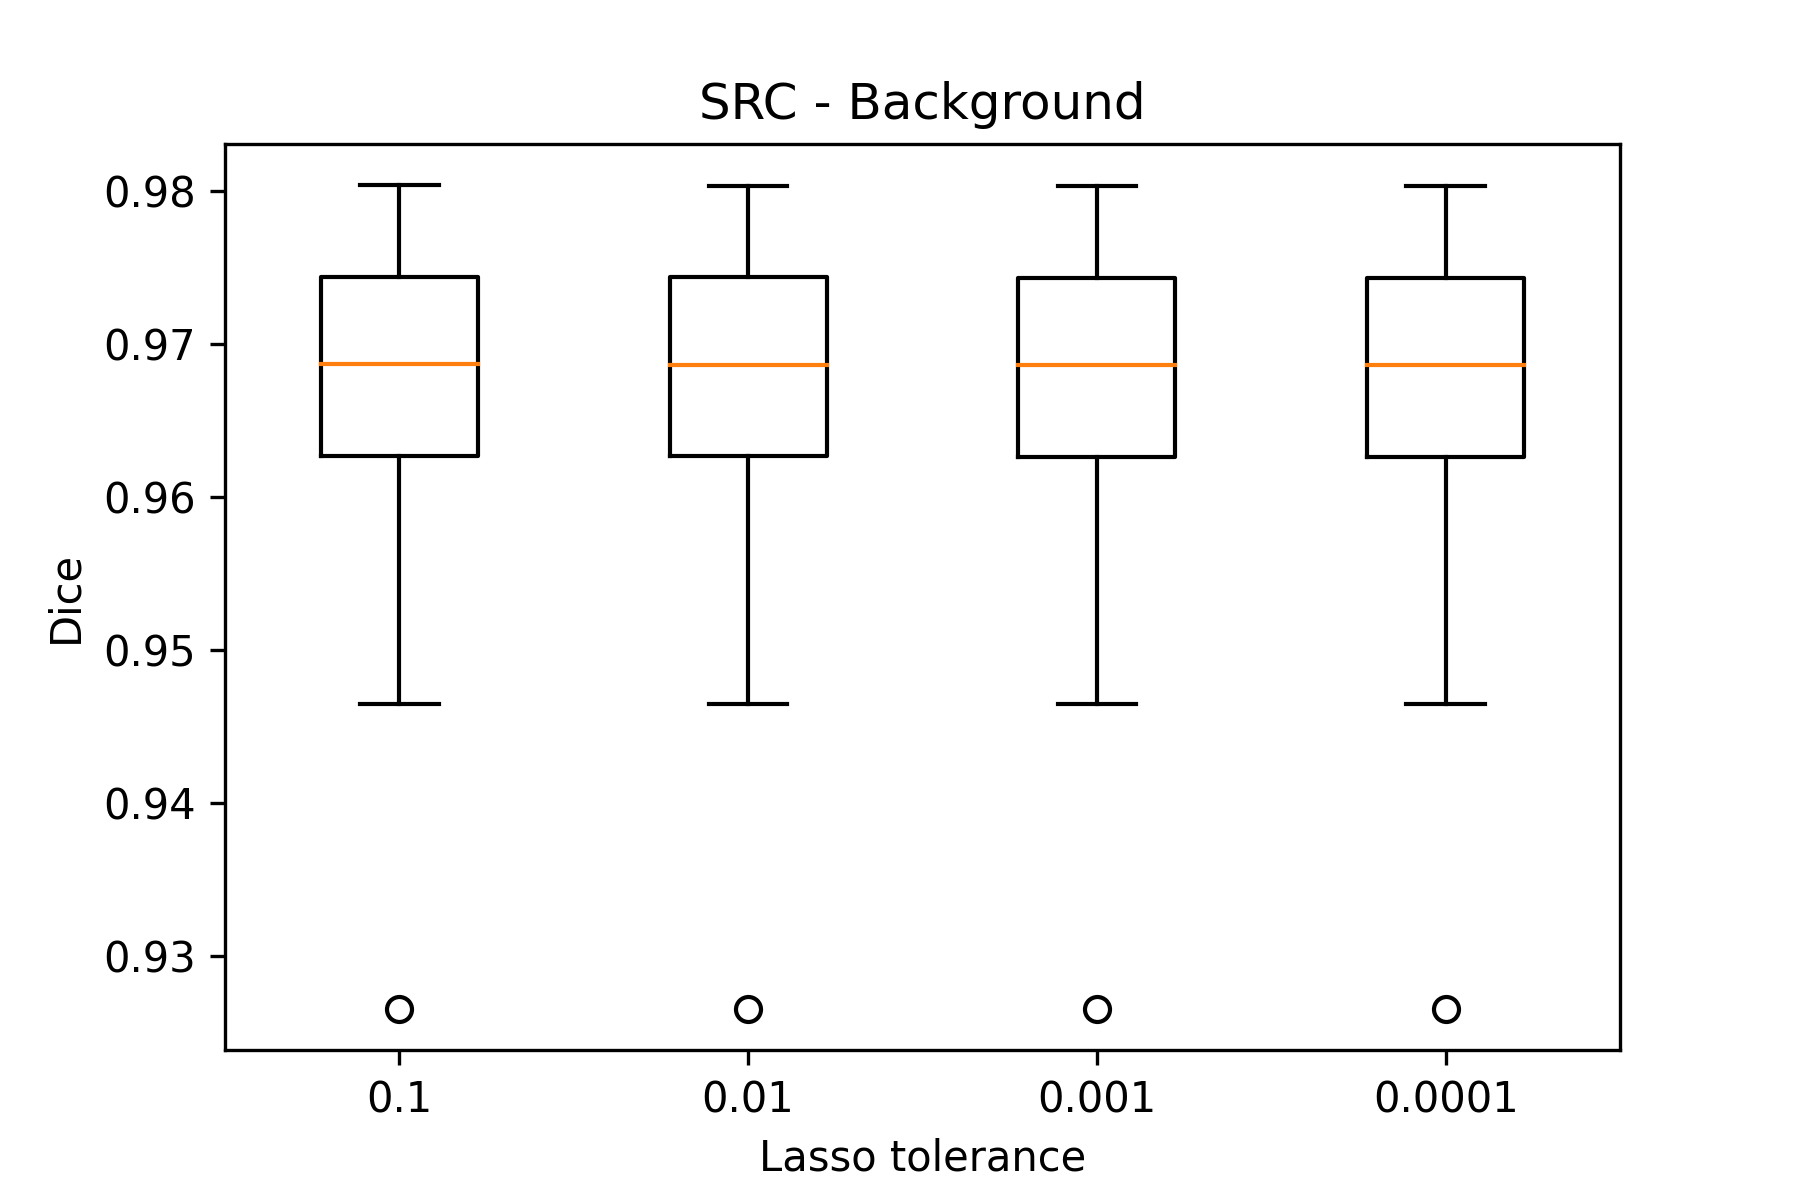
\includegraphics[width=\linewidth]{SRC_Lasso_tolerance_Background_plot.png}
    \caption{Παρασκήνιο}
    \end{subfigure}
    \begin{subfigure}[b]{0.42\linewidth}
    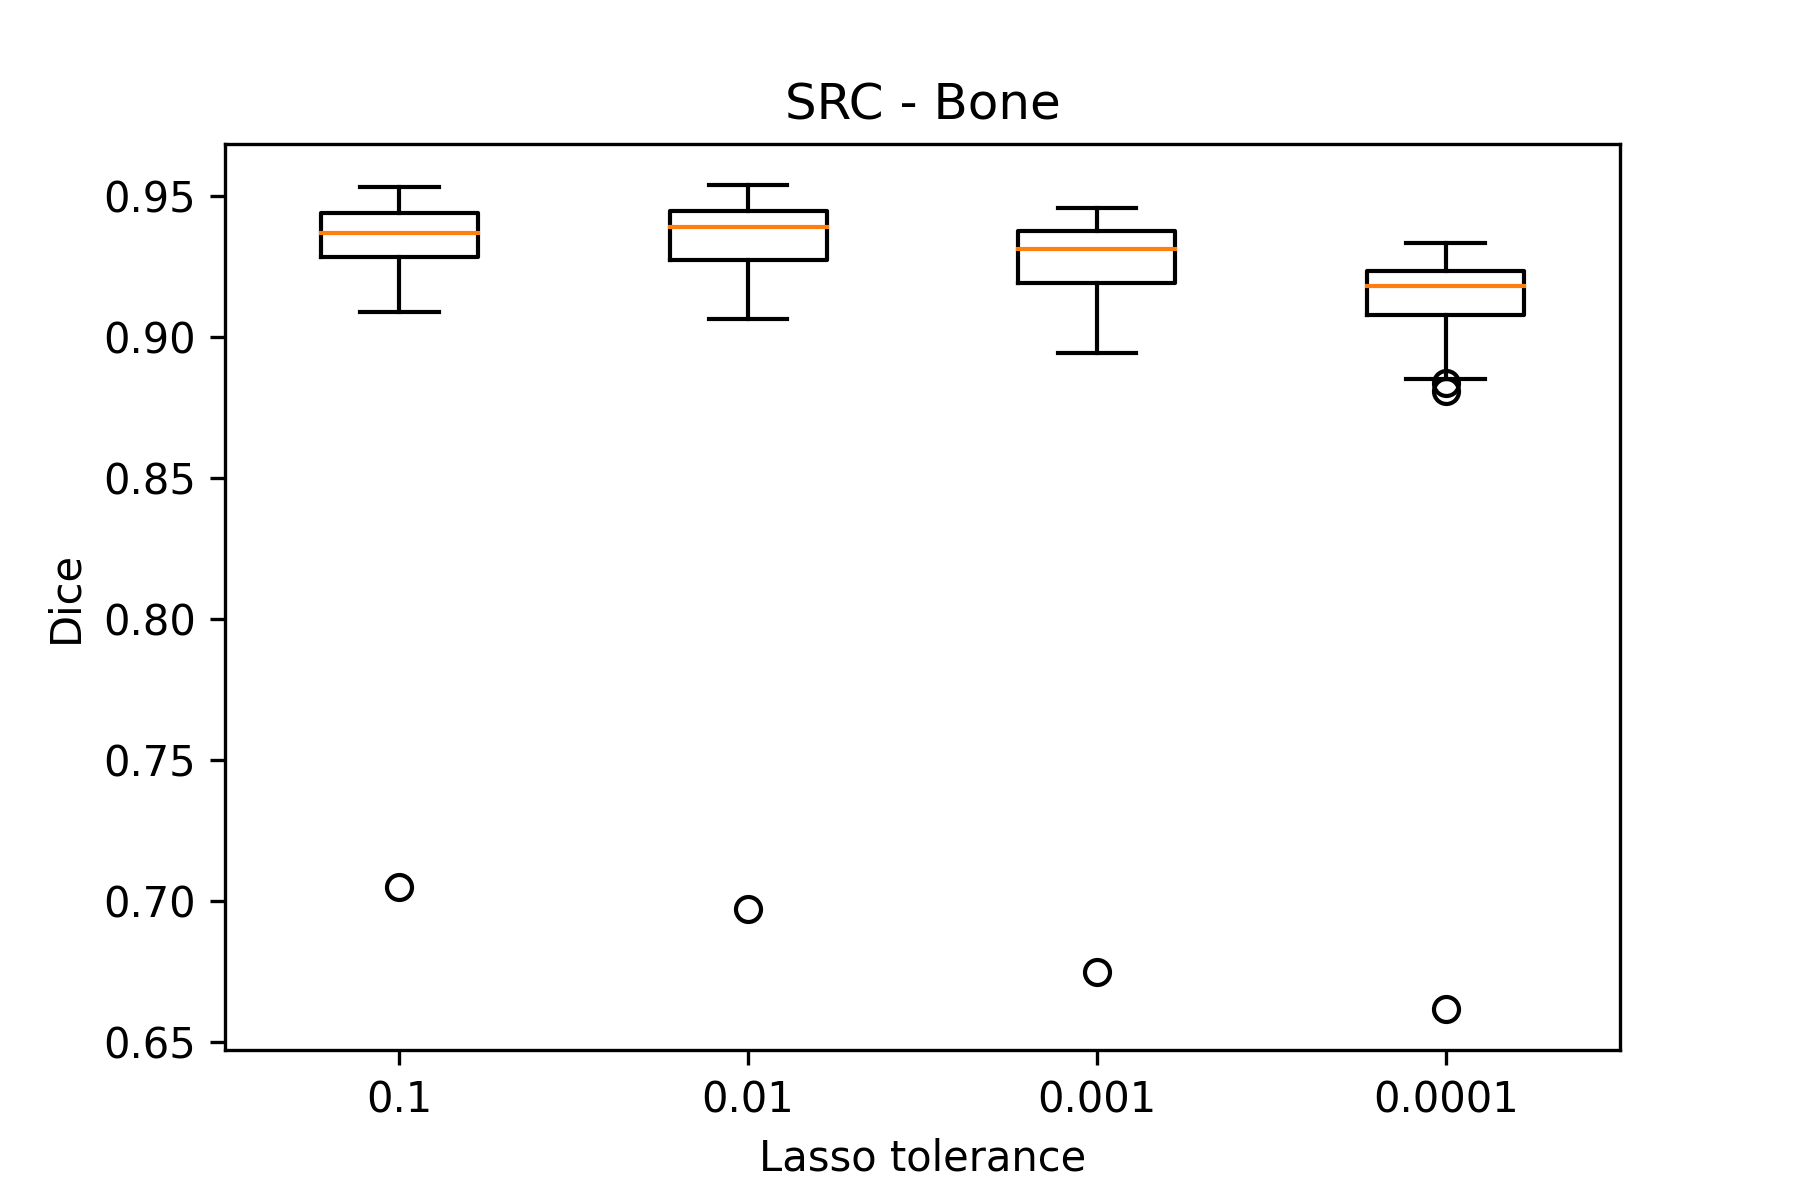
\includegraphics[width=\linewidth]{SRC_Lasso_tolerance_Bone_plot.png}
    \caption{Οστά}
    \end{subfigure}

    \begin{subfigure}[b]{0.42\linewidth}
    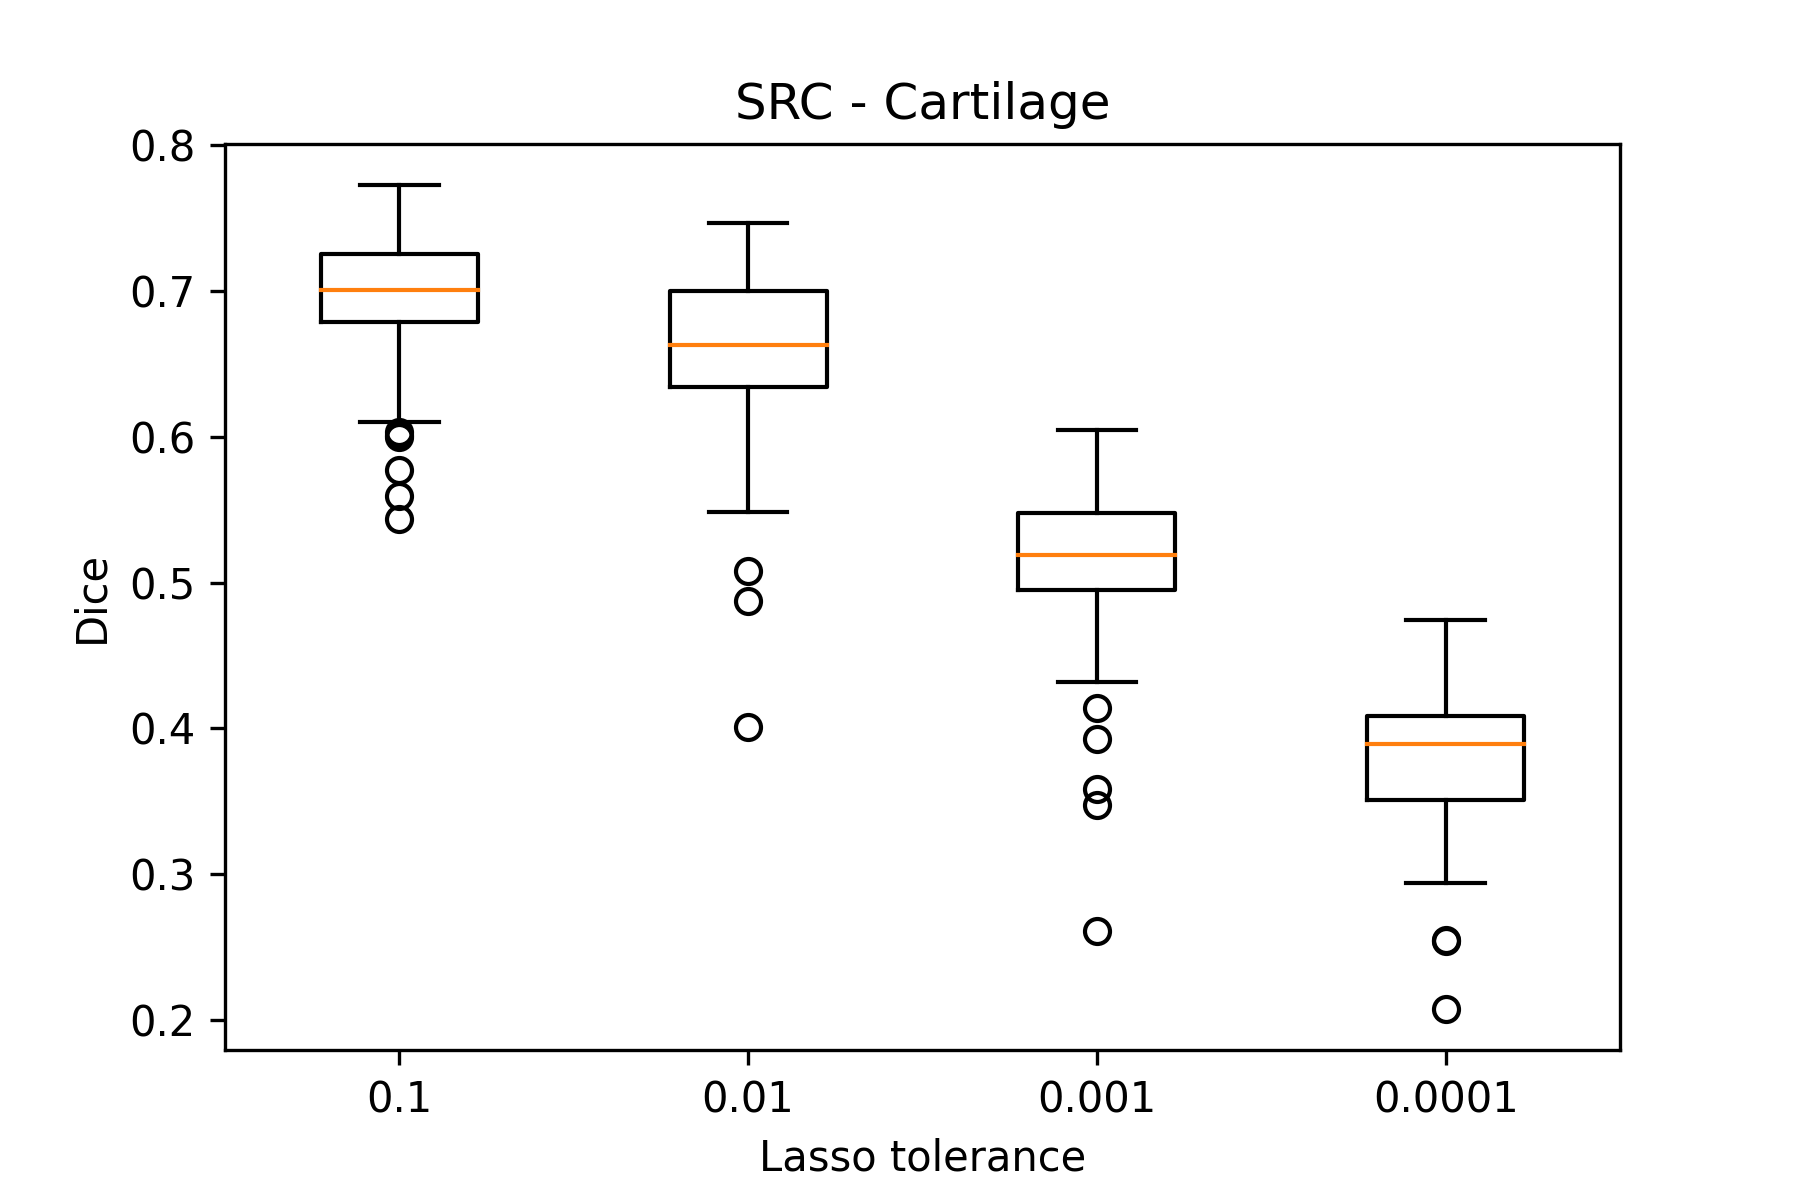
\includegraphics[width=\linewidth]{SRC_Lasso_tolerance_Cartilage_plot.png}
    \caption{Χόνδροι}
    \end{subfigure}
    \begin{subfigure}[b]{0.42\linewidth}
        \begin{tabular}[t]{|l|c|} 
            \multicolumn{2}{c}{\footnotesize Σταθερές παράμετροι} \\
            \hline
            \footnotesize Αριθμός ατλάντων & \footnotesize  4 \\ 
            \hline
            \footnotesize Μέγεθος περιοχής αναζήτησης & \footnotesize  [5,5,5] \\ 
            \hline
            \footnotesize Μέγεθος patch & \footnotesize [3,3,3] \\
            \hline
            \multicolumn{2}{c}{\footnotesize Επιλογή παραμέτρου} \\
            \hline
            \footnotesize Παράμετρος $\lambda$ & \footnotesize 0.1 \\
            \hline
        \end{tabular}
    \caption{Παράμετροι}
    \end{subfigure}
\end{figure}

\end{frame}


\begin{frame}
\frametitle{Διασταυρωμένη επικύρωση του μεγέθους της περιοχής αναζήτησης}
\framesubtitle{Μέθοδος 1: Αραιή μέθοδος βασισμένη σε τμήματα (SPBM)}

\begin{figure}[H]
    \centering

    \begin{subfigure}[b]{0.42\linewidth}
    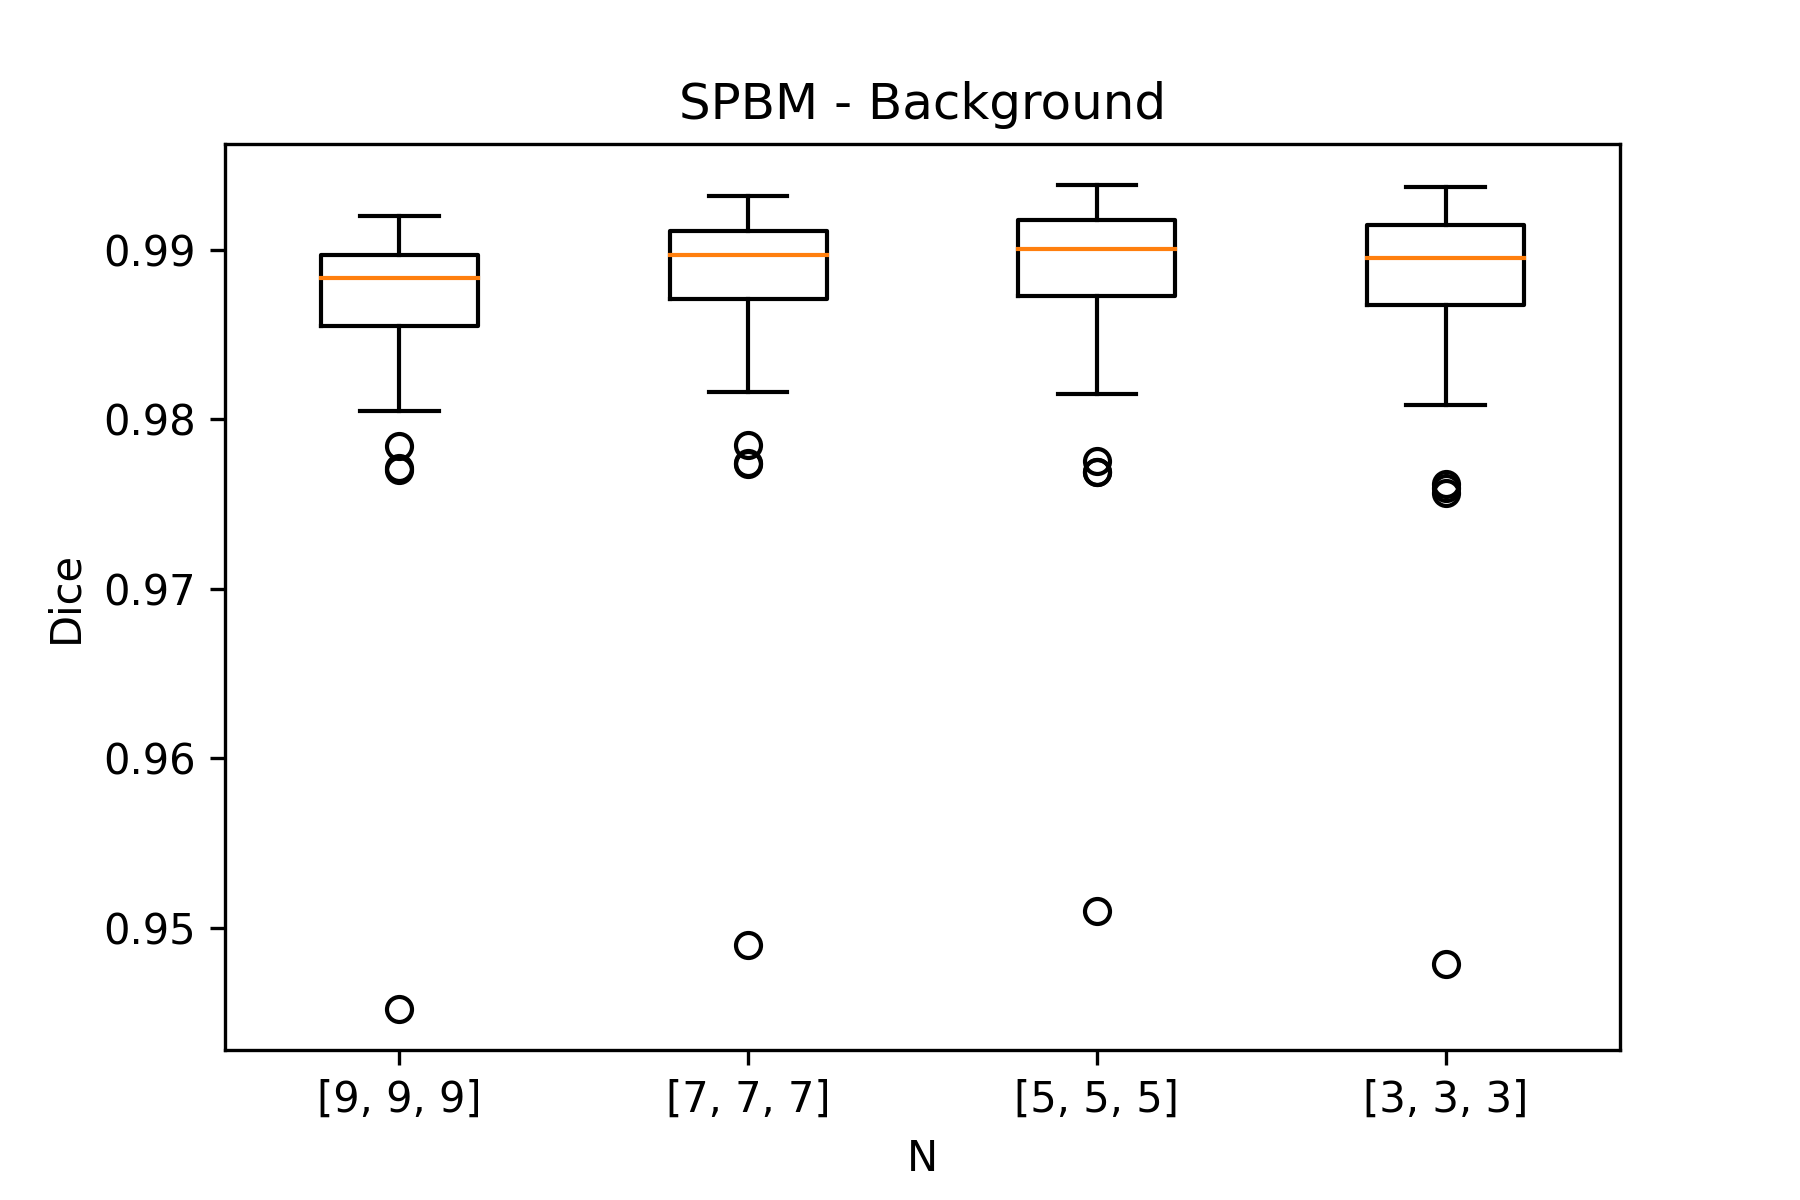
\includegraphics[width=\linewidth]{SPBM_N_Background_plot.png}
    \caption{Παρασκήνιο}
    \end{subfigure}
    \begin{subfigure}[b]{0.42\linewidth}
    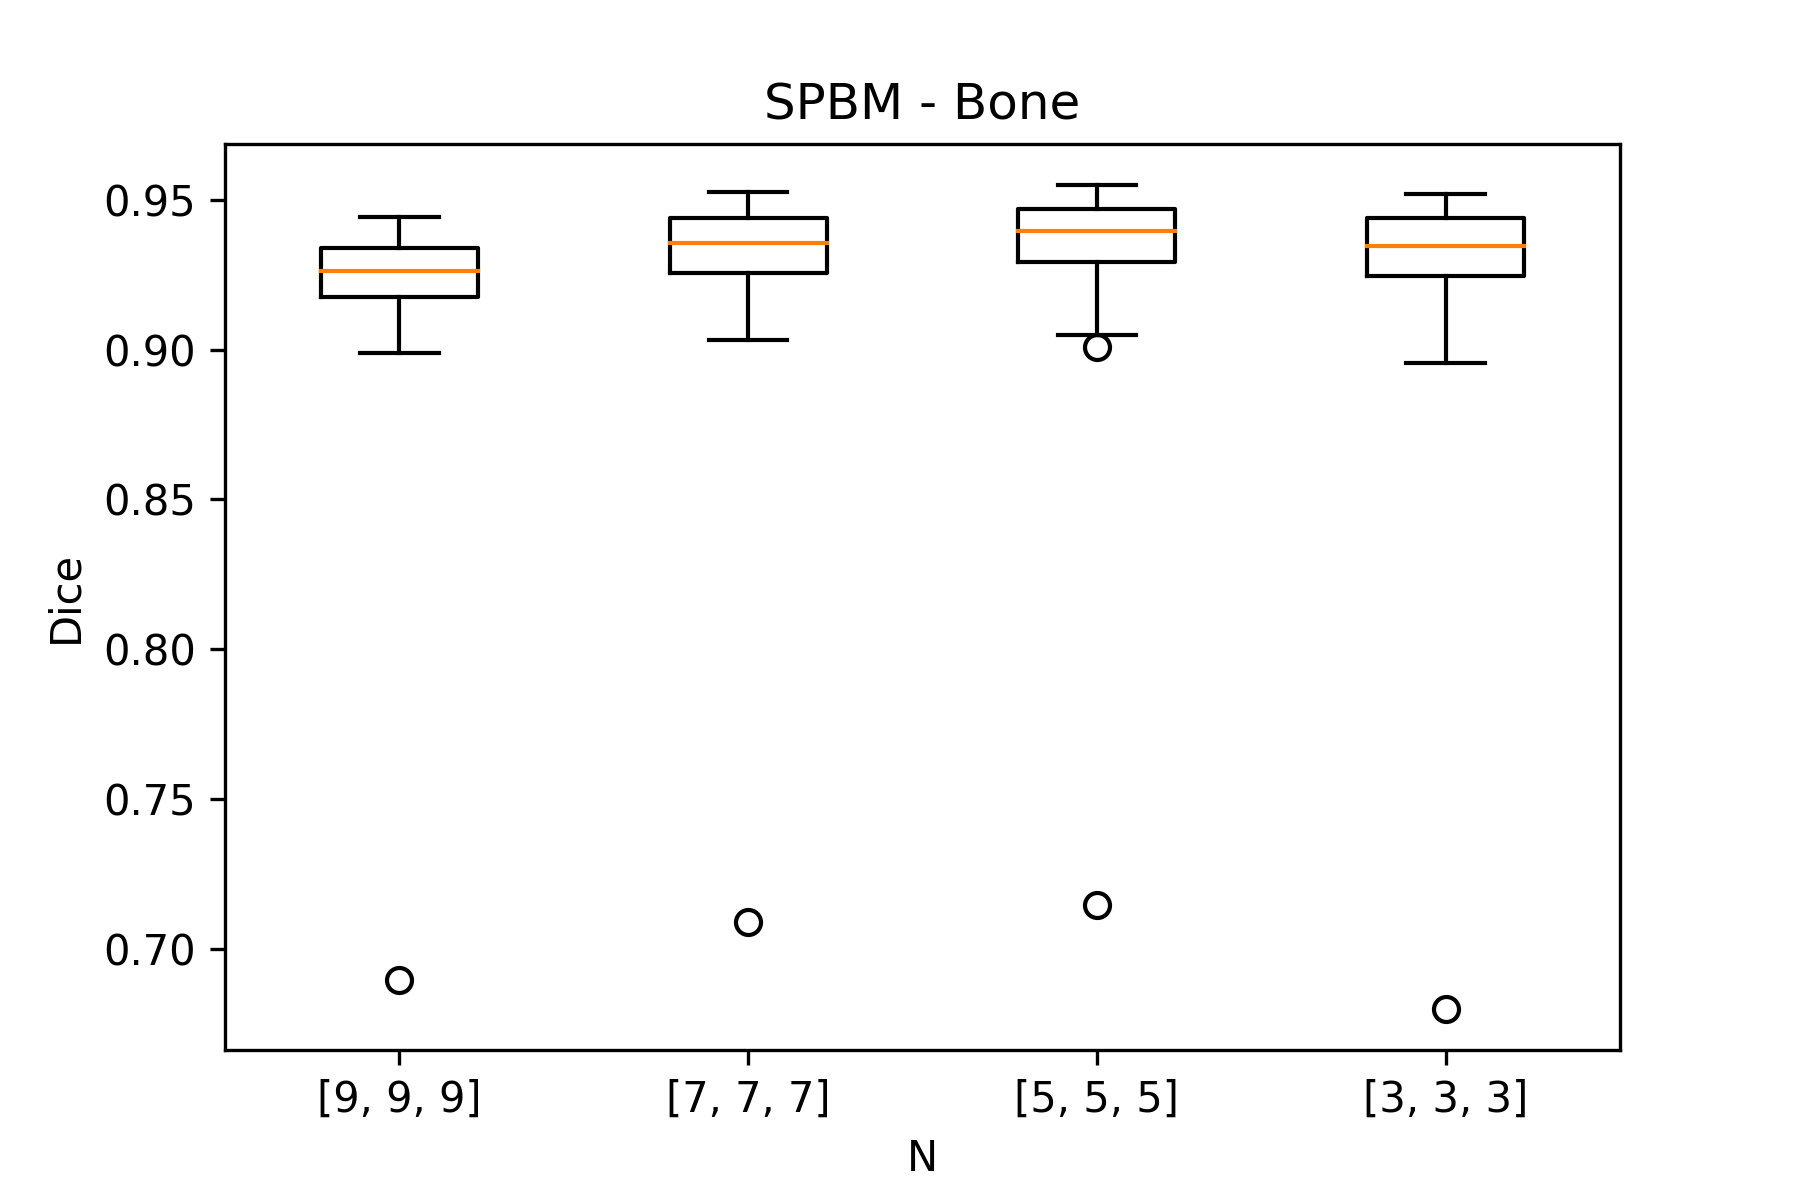
\includegraphics[width=\linewidth]{SPBM_N_Bone_plot.png}
    \caption{Οστά}
    \end{subfigure}

    \begin{subfigure}[b]{0.42\linewidth}
    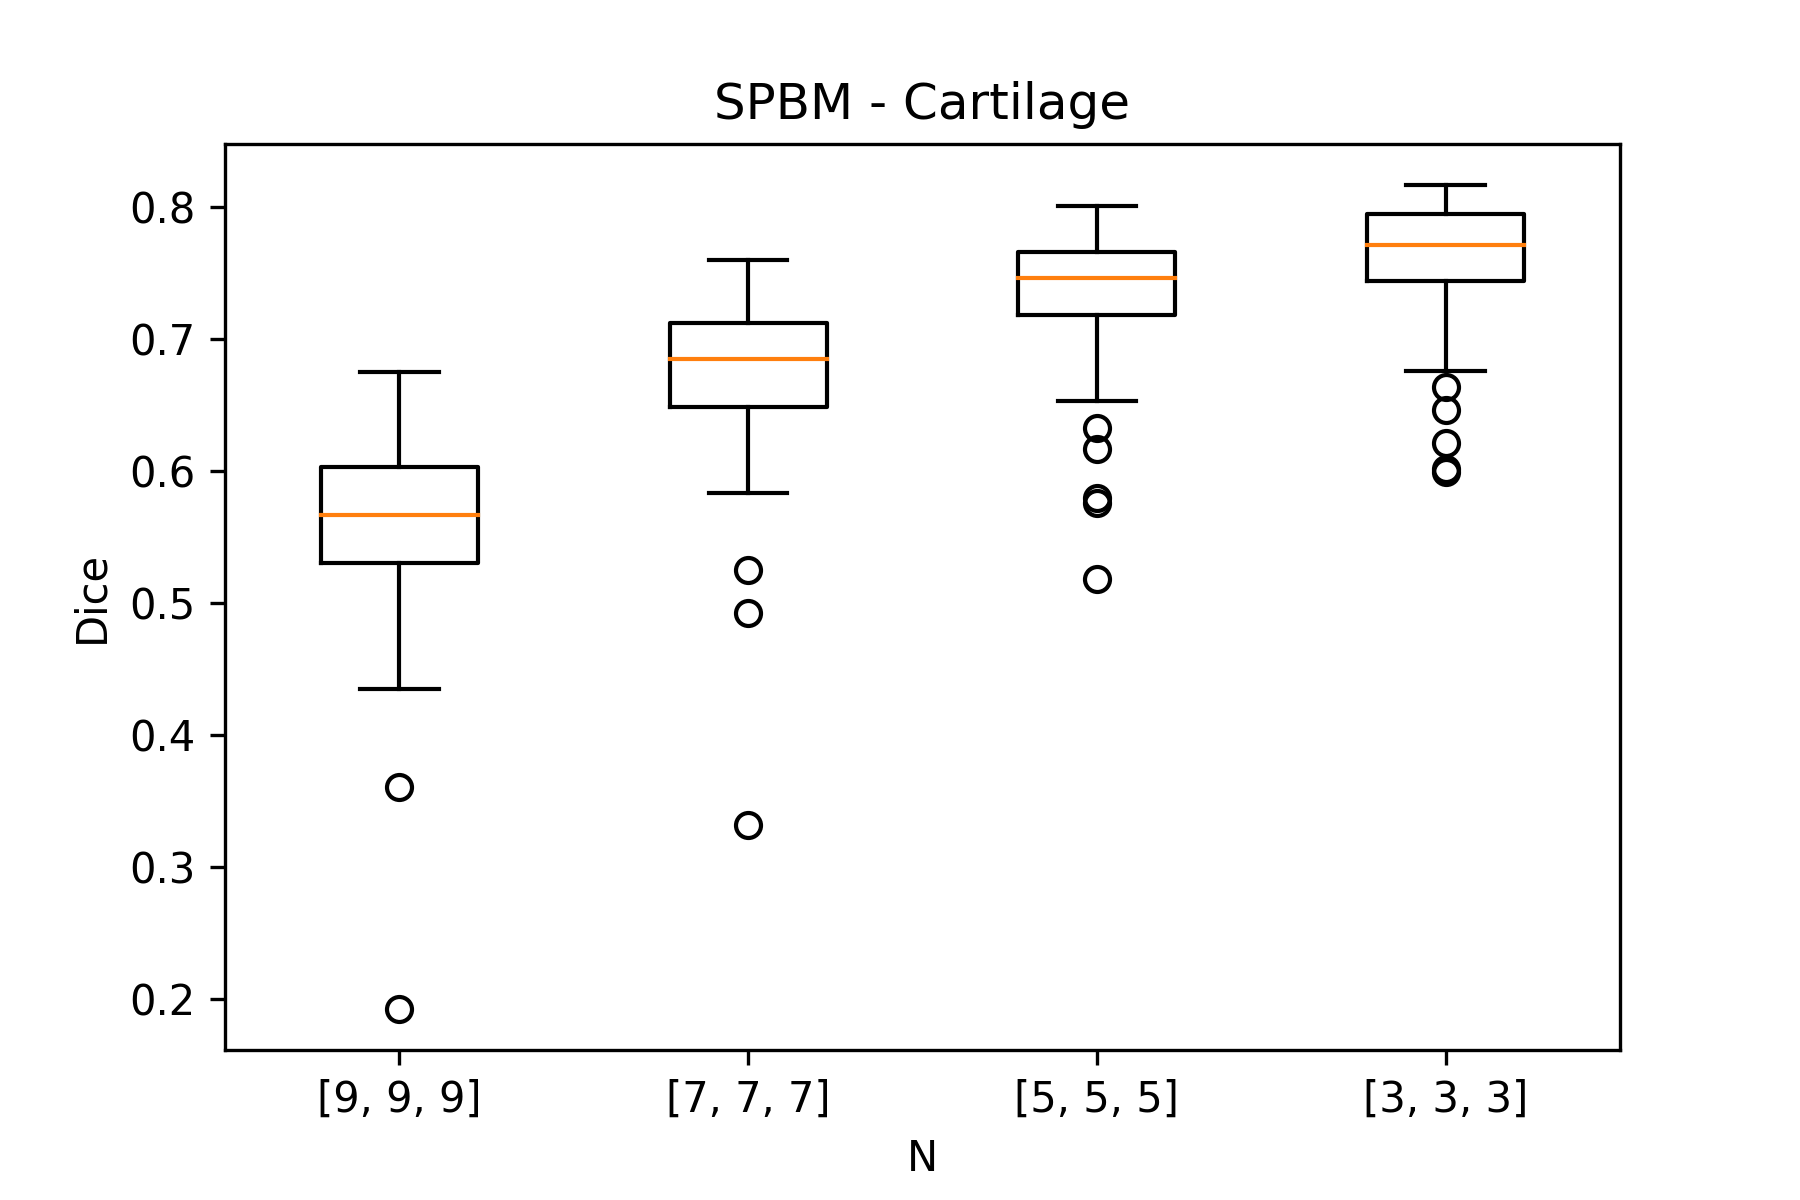
\includegraphics[width=\linewidth]{SPBM_N_Cartilage_plot.png}
    \caption{Χόνδροι}
    \end{subfigure}
    \begin{subfigure}[b]{0.42\linewidth}
        \begin{tabular}[t]{|l|c|} 
            \multicolumn{2}{c}{\footnotesize Σταθερές παράμετροι} \\
            \hline
            \footnotesize Παράμετρος $\lambda$ & \footnotesize 0.01 \\
            \hline
            \footnotesize Μέγεθος patch & \footnotesize [3,3,3] \\
            \hline
            \footnotesize Αριθμός ατλάντων & \footnotesize 4 \\ 
            \hline
            \multicolumn{2}{c}{\footnotesize Επιλογή παραμέτρου} \\
            \hline
            \footnotesize Μέγεθος περιοχής αναζήτησης & \footnotesize  [3,3,3] \\ 
            \hline
        \end{tabular}
    \caption{Παράμετροι}
    \end{subfigure}
\end{figure}

\end{frame}


\begin{frame}
\frametitle{Διασταυρωμένη επικύρωση του μεγέθους της περιοχής αναζήτησης}
\framesubtitle{Μέθοδος 2: Ταξινόμηση αραιής αναπαράστασης (SRC)}

\begin{figure}[H]
    \centering

    \begin{subfigure}[b]{0.42\linewidth}
    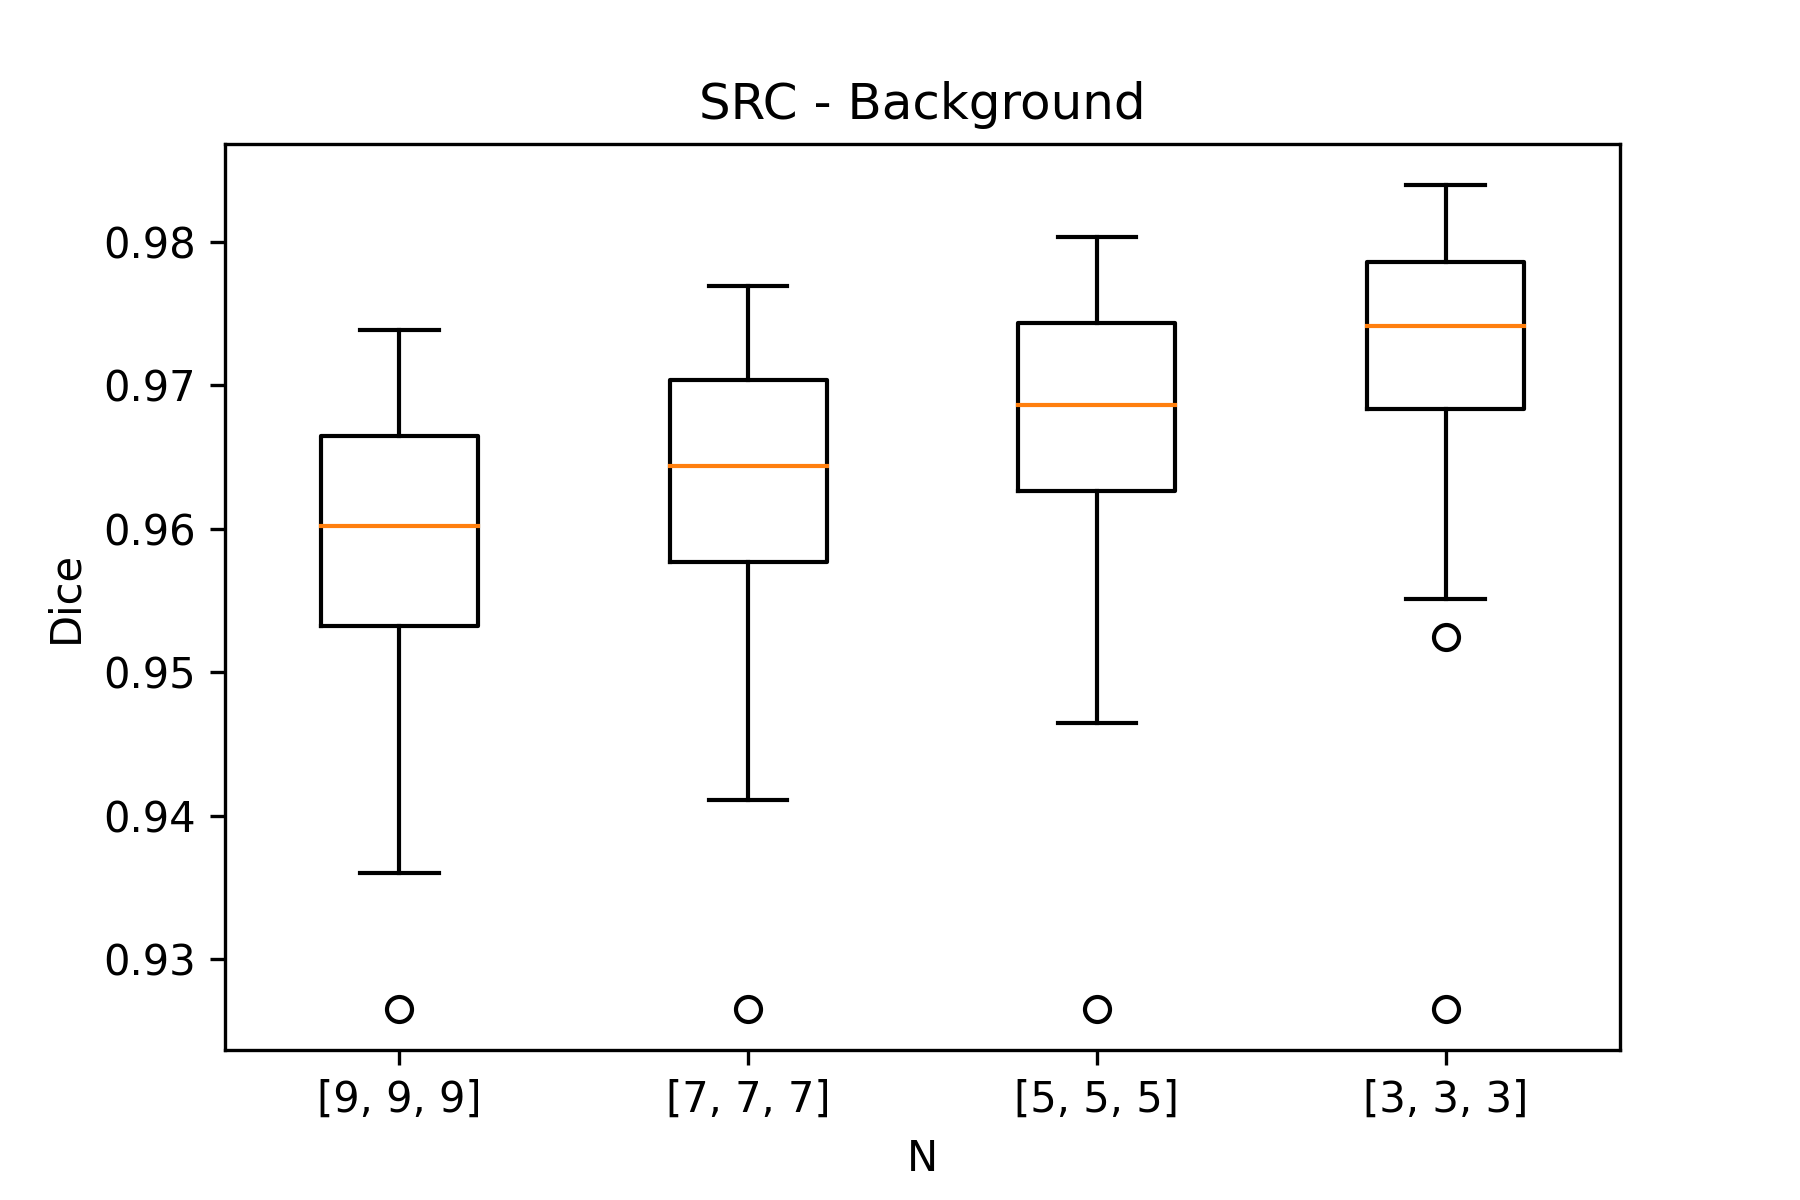
\includegraphics[width=\linewidth]{SRC_N_Background_plot.png}
    \caption{Παρασκήνιο}
    \end{subfigure}
    \begin{subfigure}[b]{0.42\linewidth}
    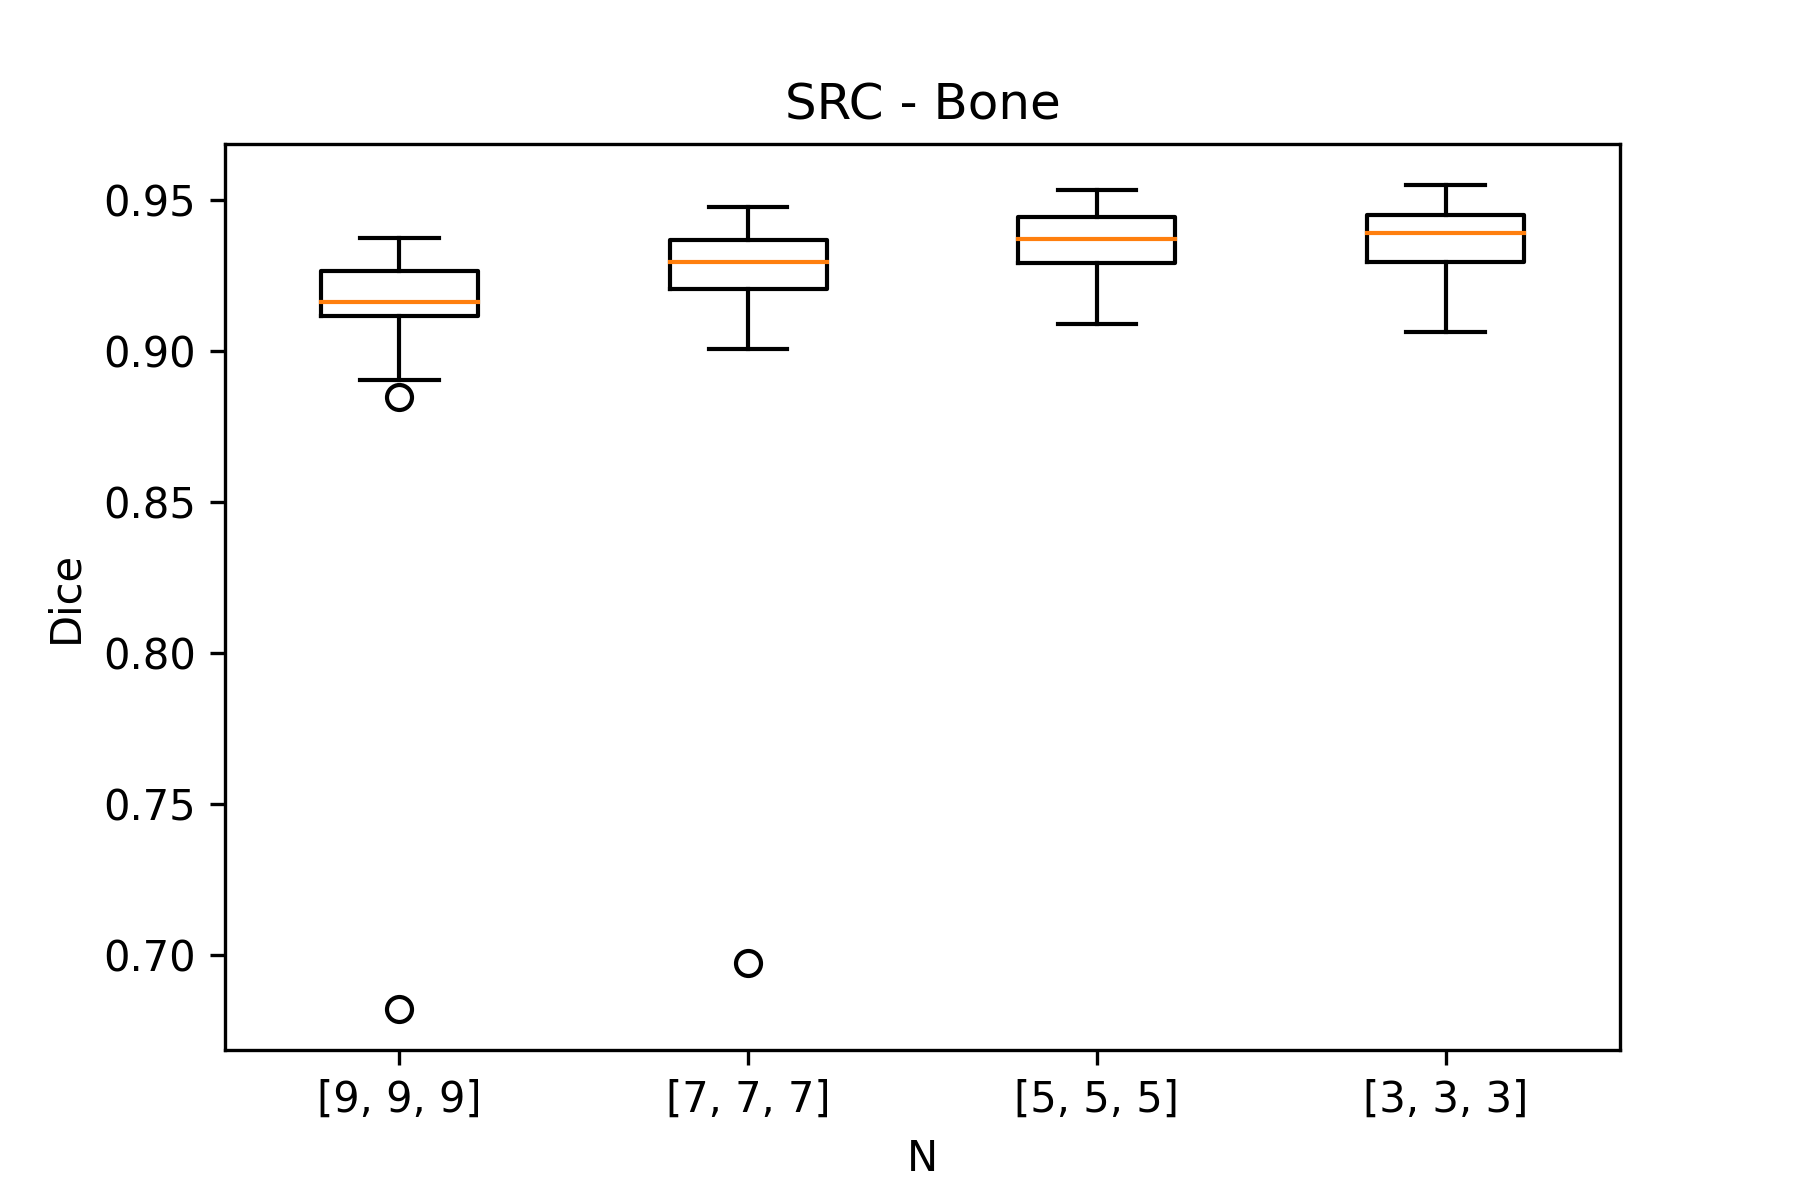
\includegraphics[width=\linewidth]{SRC_N_Bone_plot.png}
    \caption{Οστά}
    \end{subfigure}

    \begin{subfigure}[b]{0.42\linewidth}
    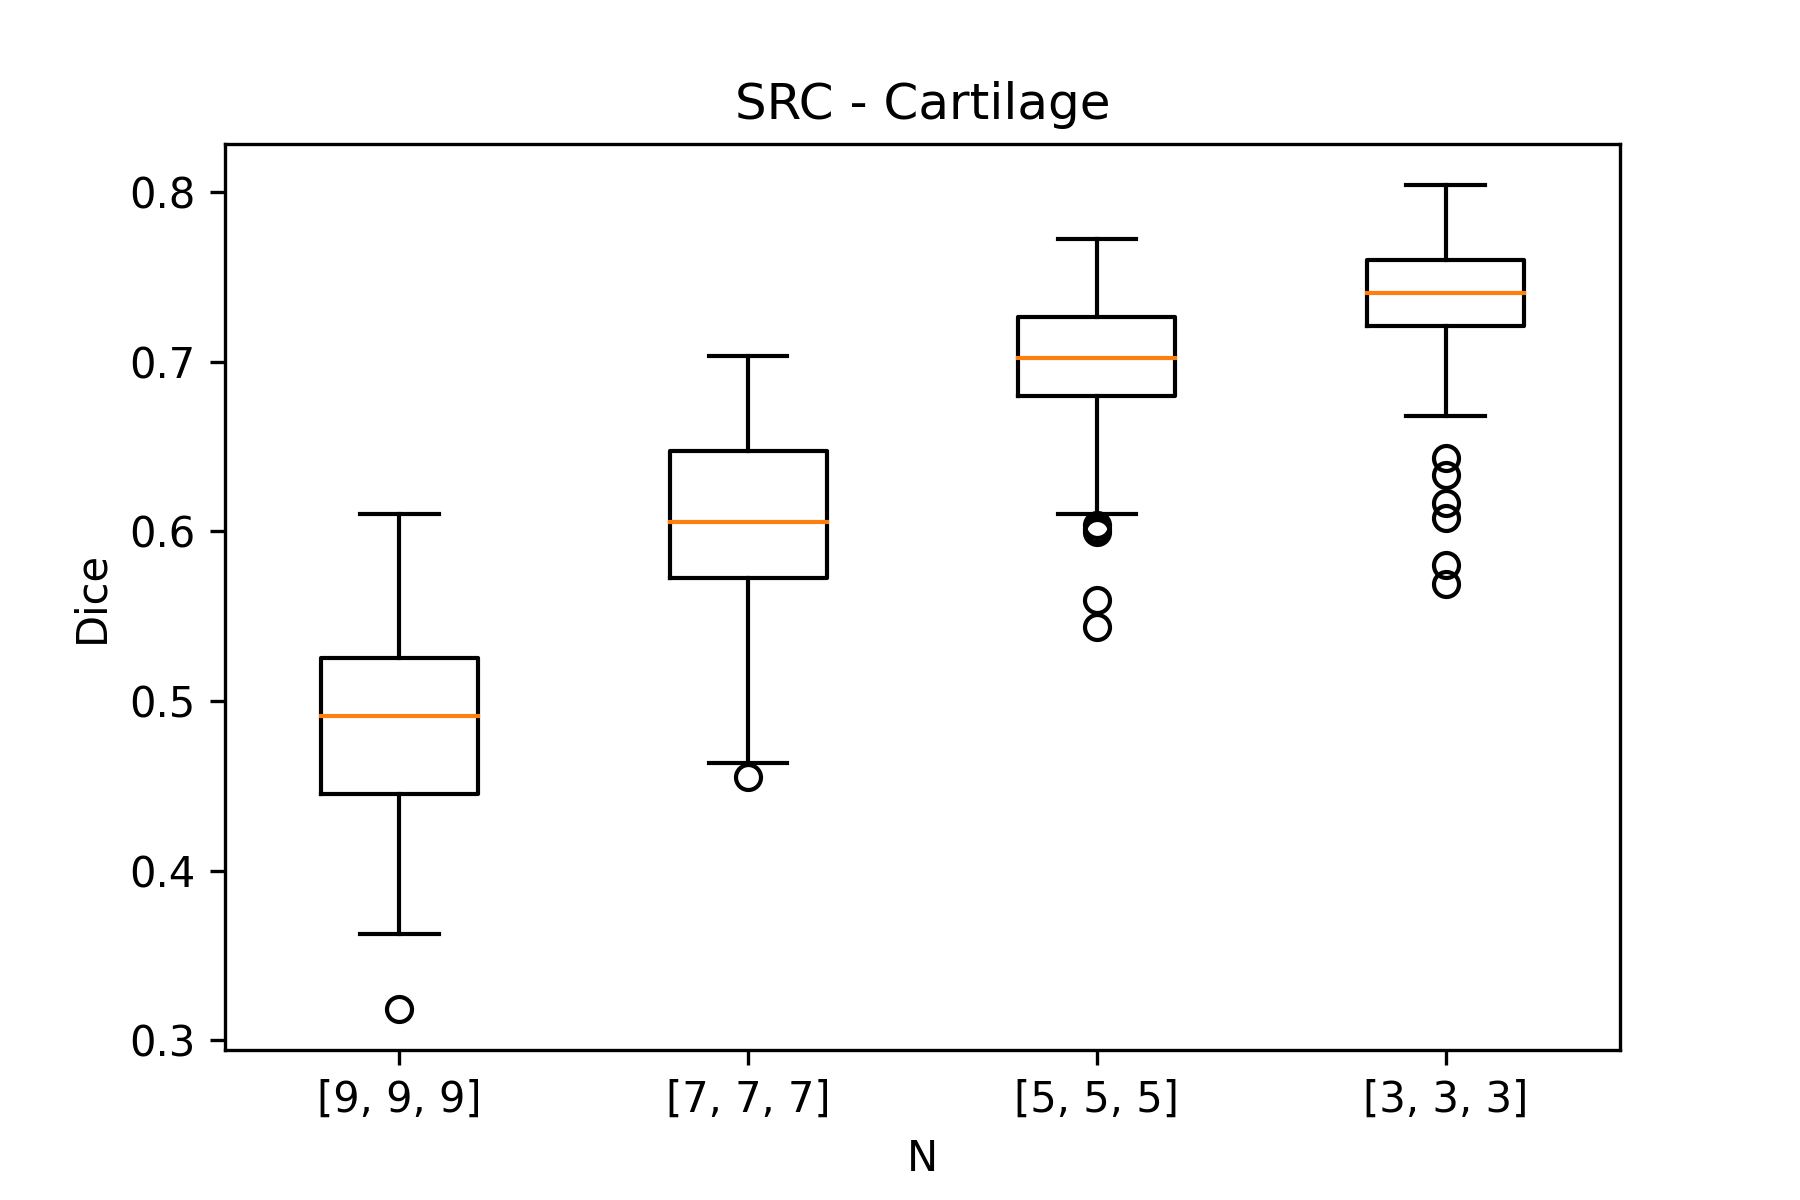
\includegraphics[width=\linewidth]{SRC_N_Cartilage_plot.png}
    \caption{Χόνδροι}
    \end{subfigure}
    \begin{subfigure}[b]{0.42\linewidth}
        \begin{tabular}[t]{|l|c|} 
            \multicolumn{2}{c}{\footnotesize Σταθερές παράμετροι} \\
            \hline
            \footnotesize Παράμετρος $\lambda$ & \footnotesize 0.1 \\
            \hline
            \footnotesize Μέγεθος patch & \footnotesize [3,3,3] \\
            \hline
            \footnotesize Αριθμός ατλάντων & \footnotesize 4 \\ 
            \hline
            \multicolumn{2}{c}{\footnotesize Επιλογή παραμέτρου} \\
            \hline
            \footnotesize Μέγεθος περιοχής αναζήτησης & \footnotesize  [3,3,3] \\ 
            \hline
        \end{tabular}
    \caption{Παράμετροι}
    \end{subfigure}
\end{figure}

\end{frame}


\begin{frame}
\frametitle{Διασταυρωμένη επικύρωση του μεγέθους της περιοχής αναζήτησης}
\framesubtitle{Μέθοδος 3: Κατάτμηση βασισμένη σε τμήματα με τη χρήση πληροφορίας
από ειδικούς (PBSEP)}

\begin{figure}[H]
    \centering

    \begin{subfigure}[b]{0.42\linewidth}
    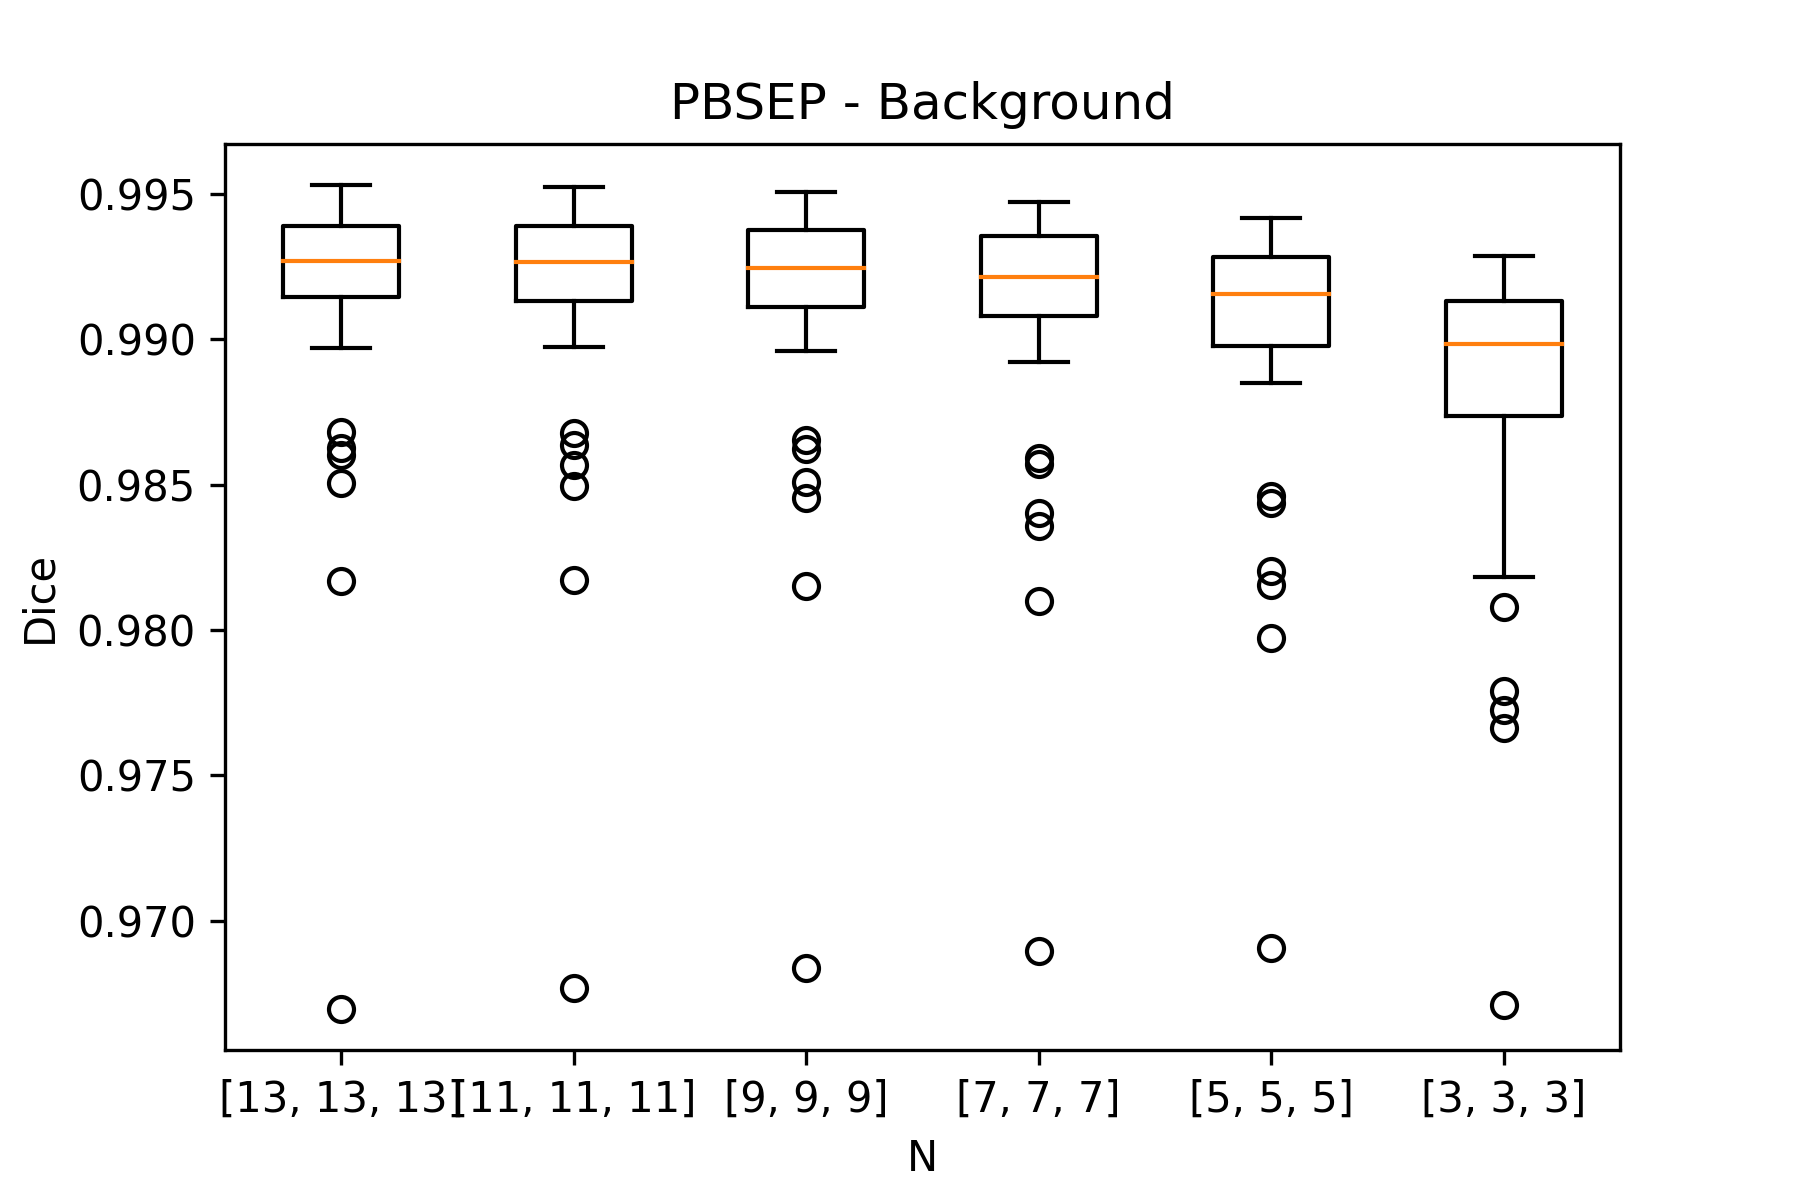
\includegraphics[width=\linewidth]{PBSEP_N_Background_plot.png}
    \caption{Παρασκήνιο}
    \end{subfigure}
    \begin{subfigure}[b]{0.42\linewidth}
    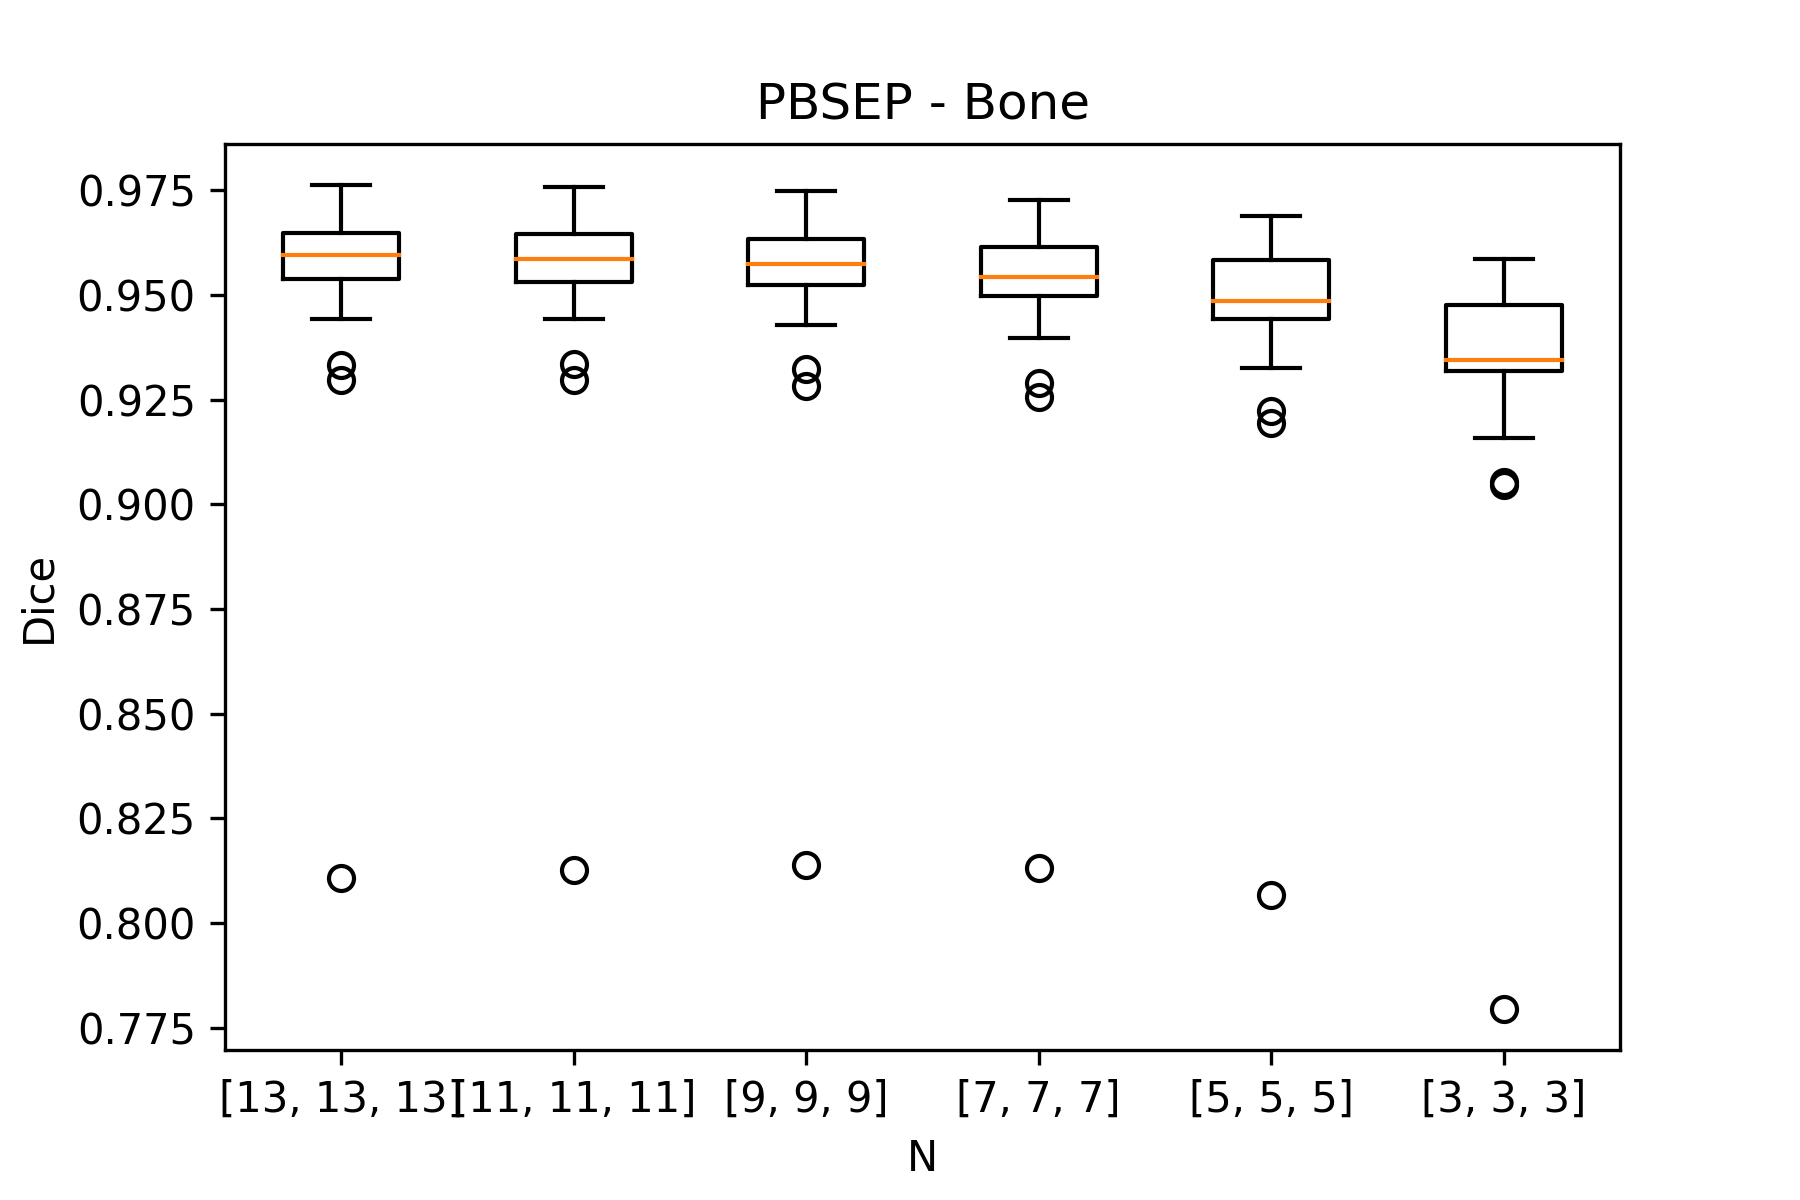
\includegraphics[width=\linewidth]{PBSEP_N_Bone_plot.png}
    \caption{Οστά}
    \end{subfigure}

    \begin{subfigure}[b]{0.42\linewidth}
    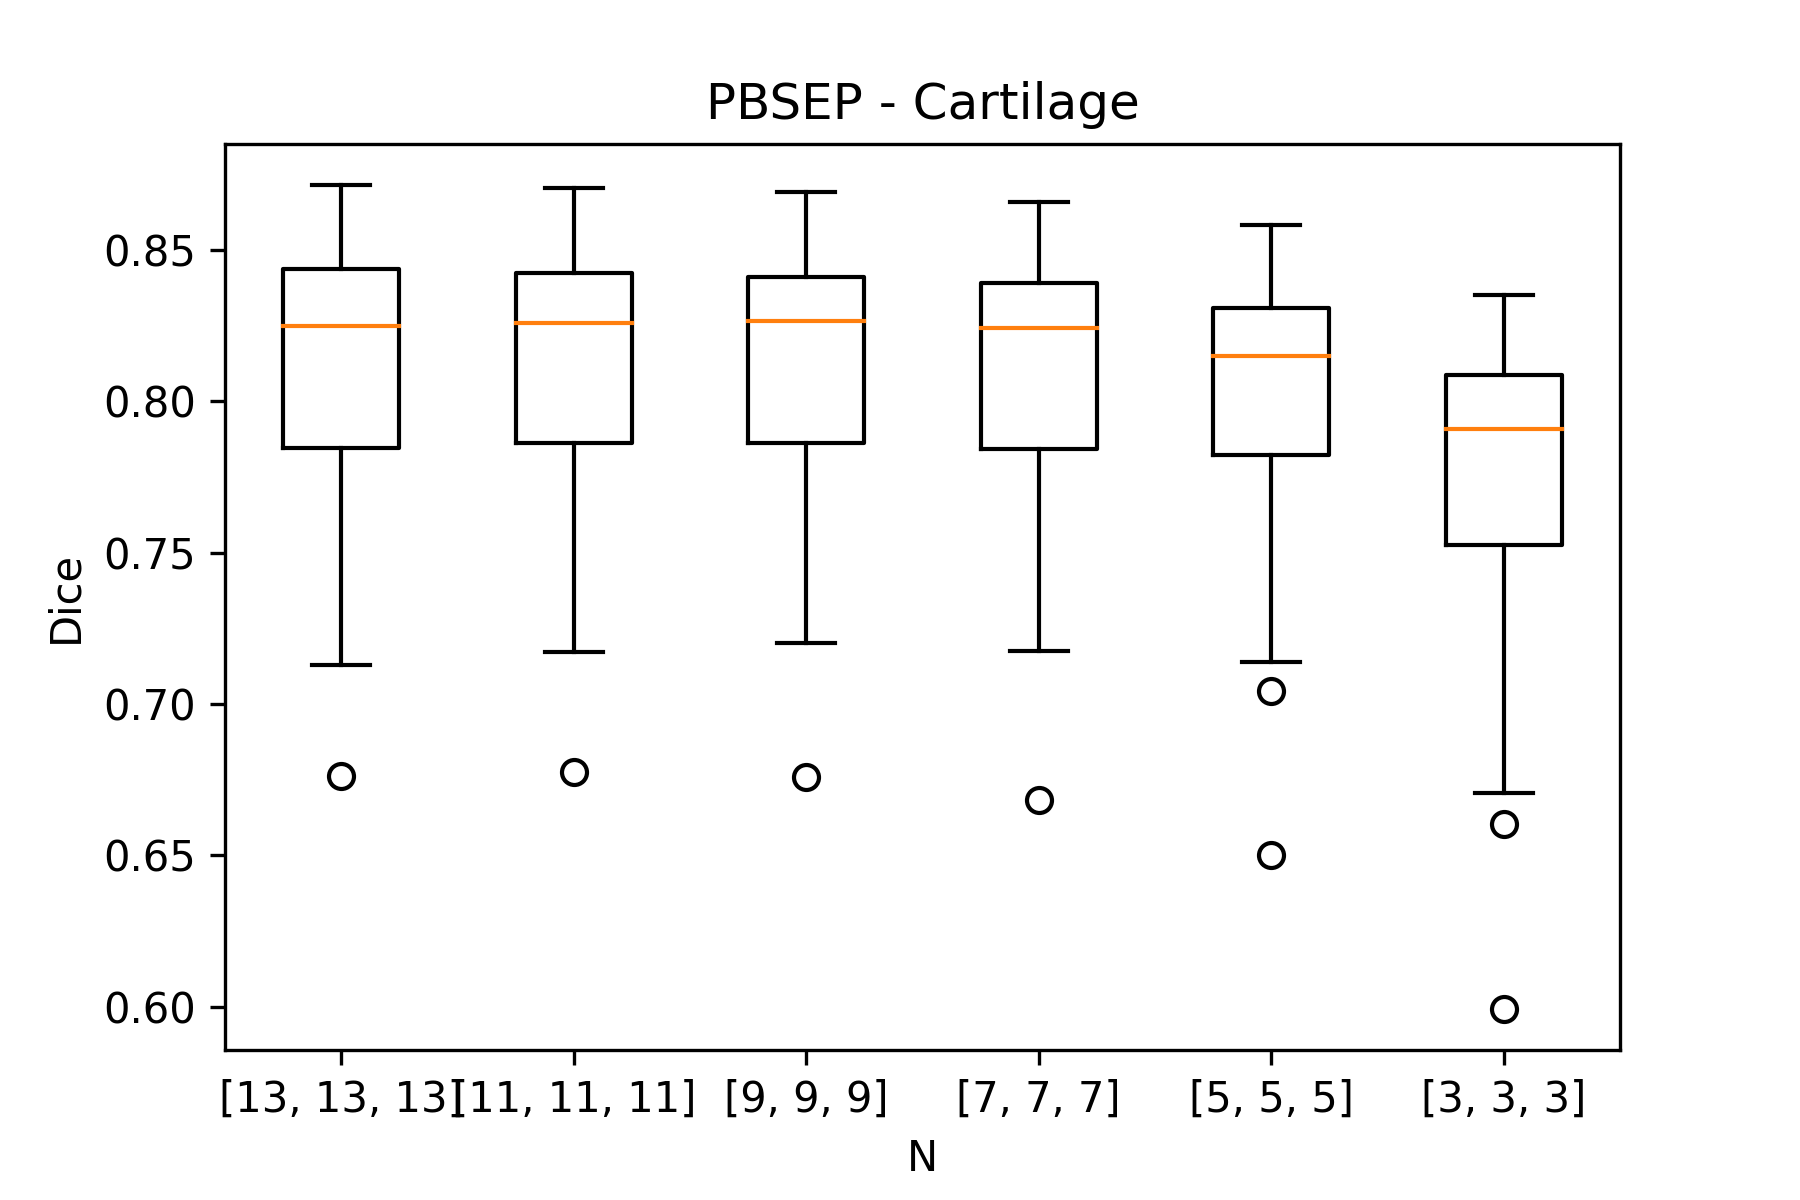
\includegraphics[width=\linewidth]{PBSEP_N_Cartilage_plot.png}
    \caption{Χόνδροι}
    \end{subfigure}
    \begin{subfigure}[b]{0.42\linewidth}
        \begin{tabular}[t]{|l|c|} 
            \multicolumn{2}{c}{\footnotesize Σταθερές παράμετροι} \\
            \hline
            \footnotesize Μέγεθος patch & \footnotesize [3,3,3] \\
            \hline
            \footnotesize Αριθμός ατλάντων & \footnotesize 4 \\ 
            \hline
            \multicolumn{2}{c}{\footnotesize Επιλογή παραμέτρου} \\
            \hline
            \footnotesize Μέγεθος περιοχής αναζήτησης & \footnotesize  [7,7,7] \\ 
            \hline
        \end{tabular}
    \caption{Παράμετροι}
    \end{subfigure}
\end{figure}

\end{frame}


\begin{frame}
\frametitle{Διασταυρωμένη επικύρωση του μεγέθους του patch}
\framesubtitle{Μέθοδος 1: Αραιή μέθοδος βασισμένη σε τμήματα (SPBM)}

\begin{figure}[H]
    \centering

    \begin{subfigure}[b]{0.42\linewidth}
    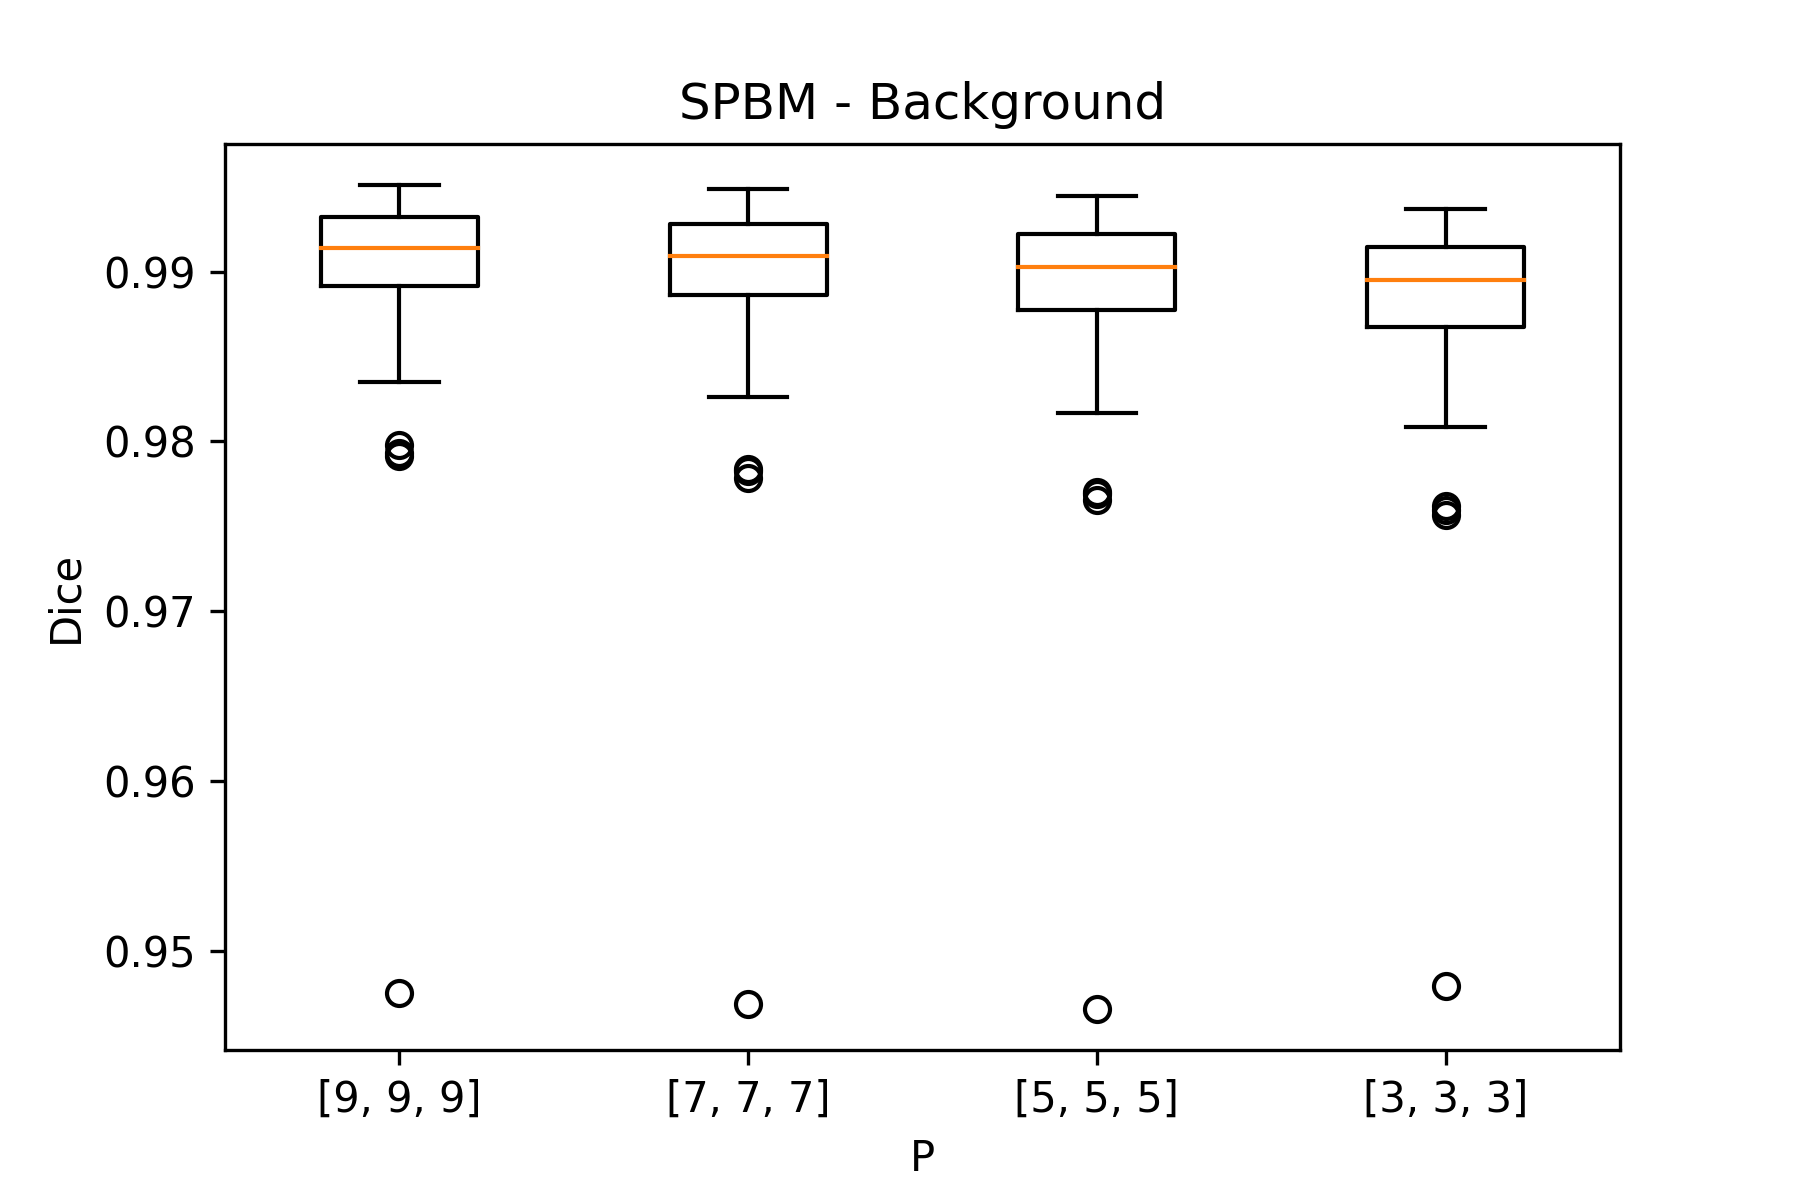
\includegraphics[width=\linewidth]{SPBM_P_Background_plot.png}
    \caption{Παρασκήνιο}
    \end{subfigure}
    \begin{subfigure}[b]{0.42\linewidth}
    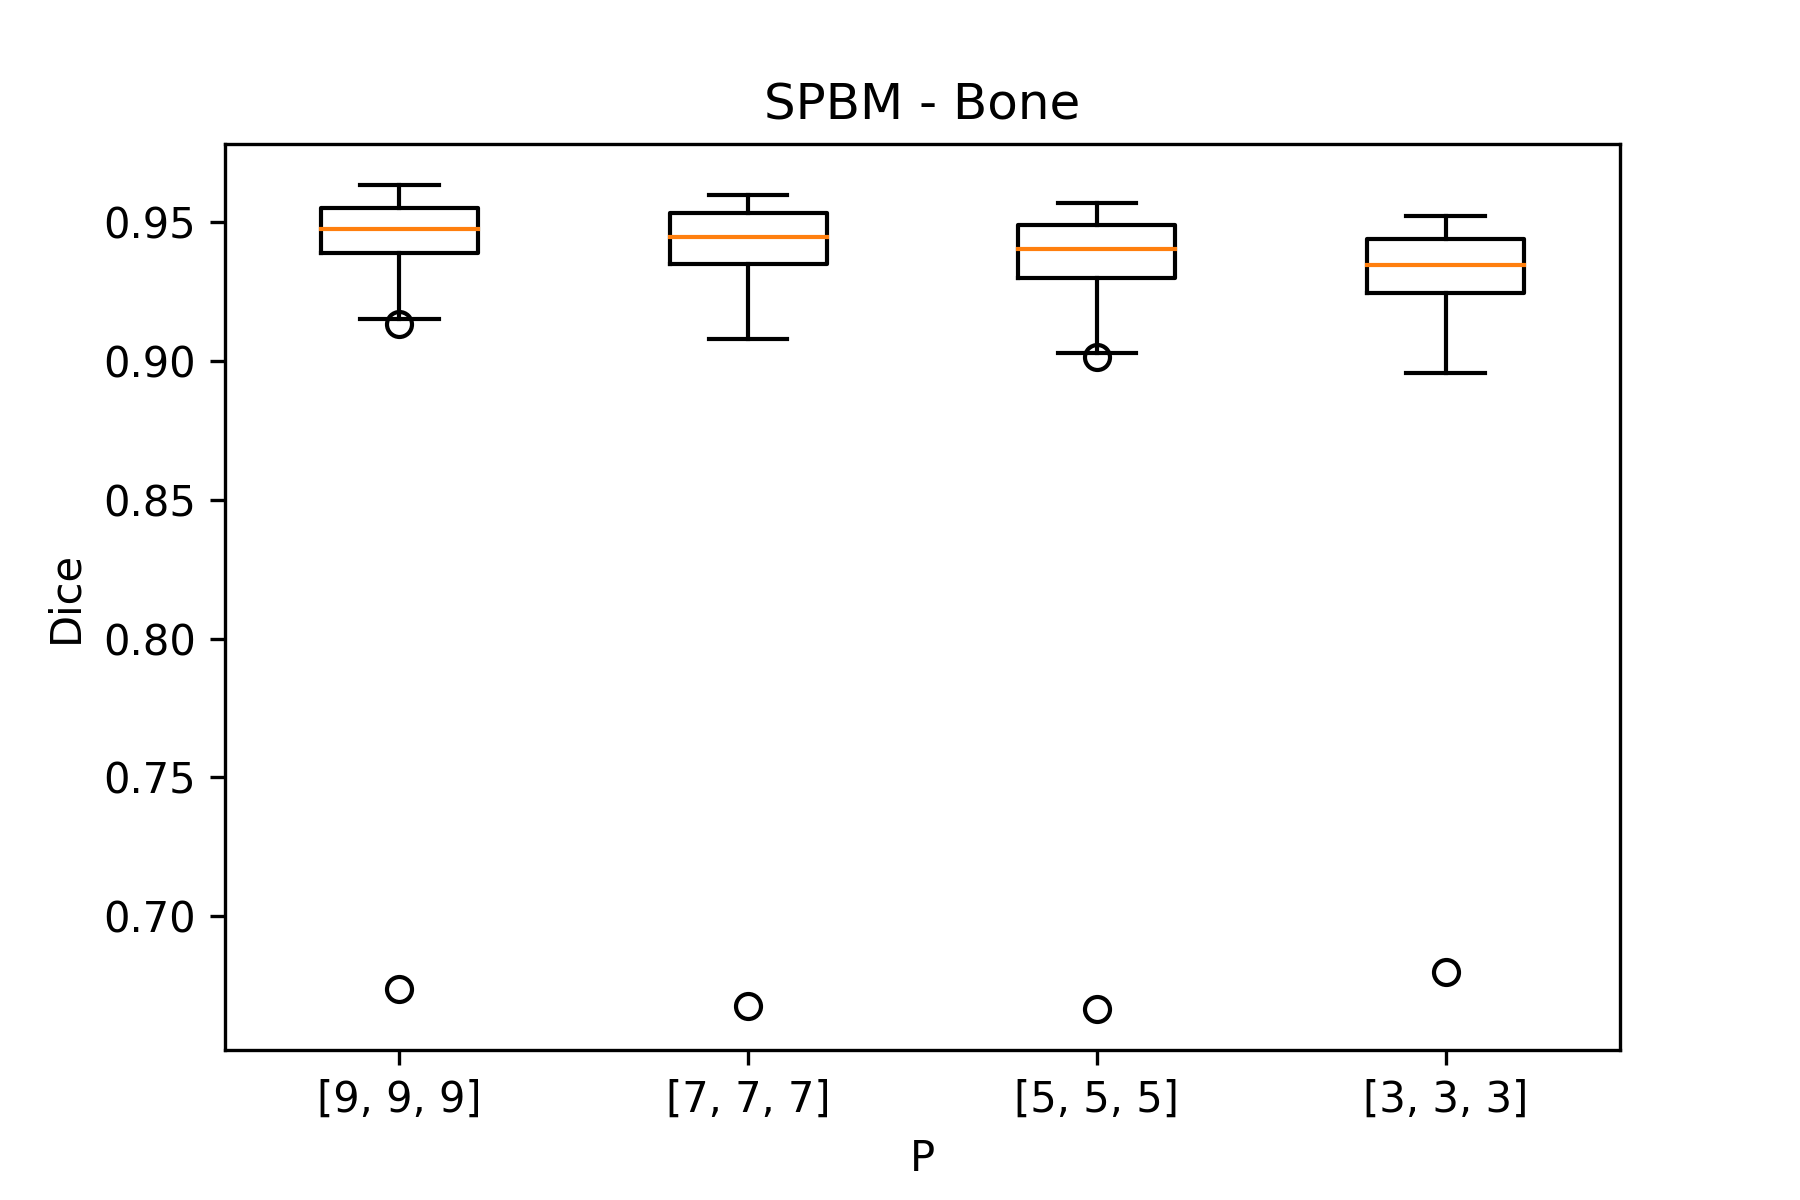
\includegraphics[width=\linewidth]{SPBM_P_Bone_plot.png}
    \caption{Οστά}
    \end{subfigure}

    \begin{subfigure}[b]{0.42\linewidth}
    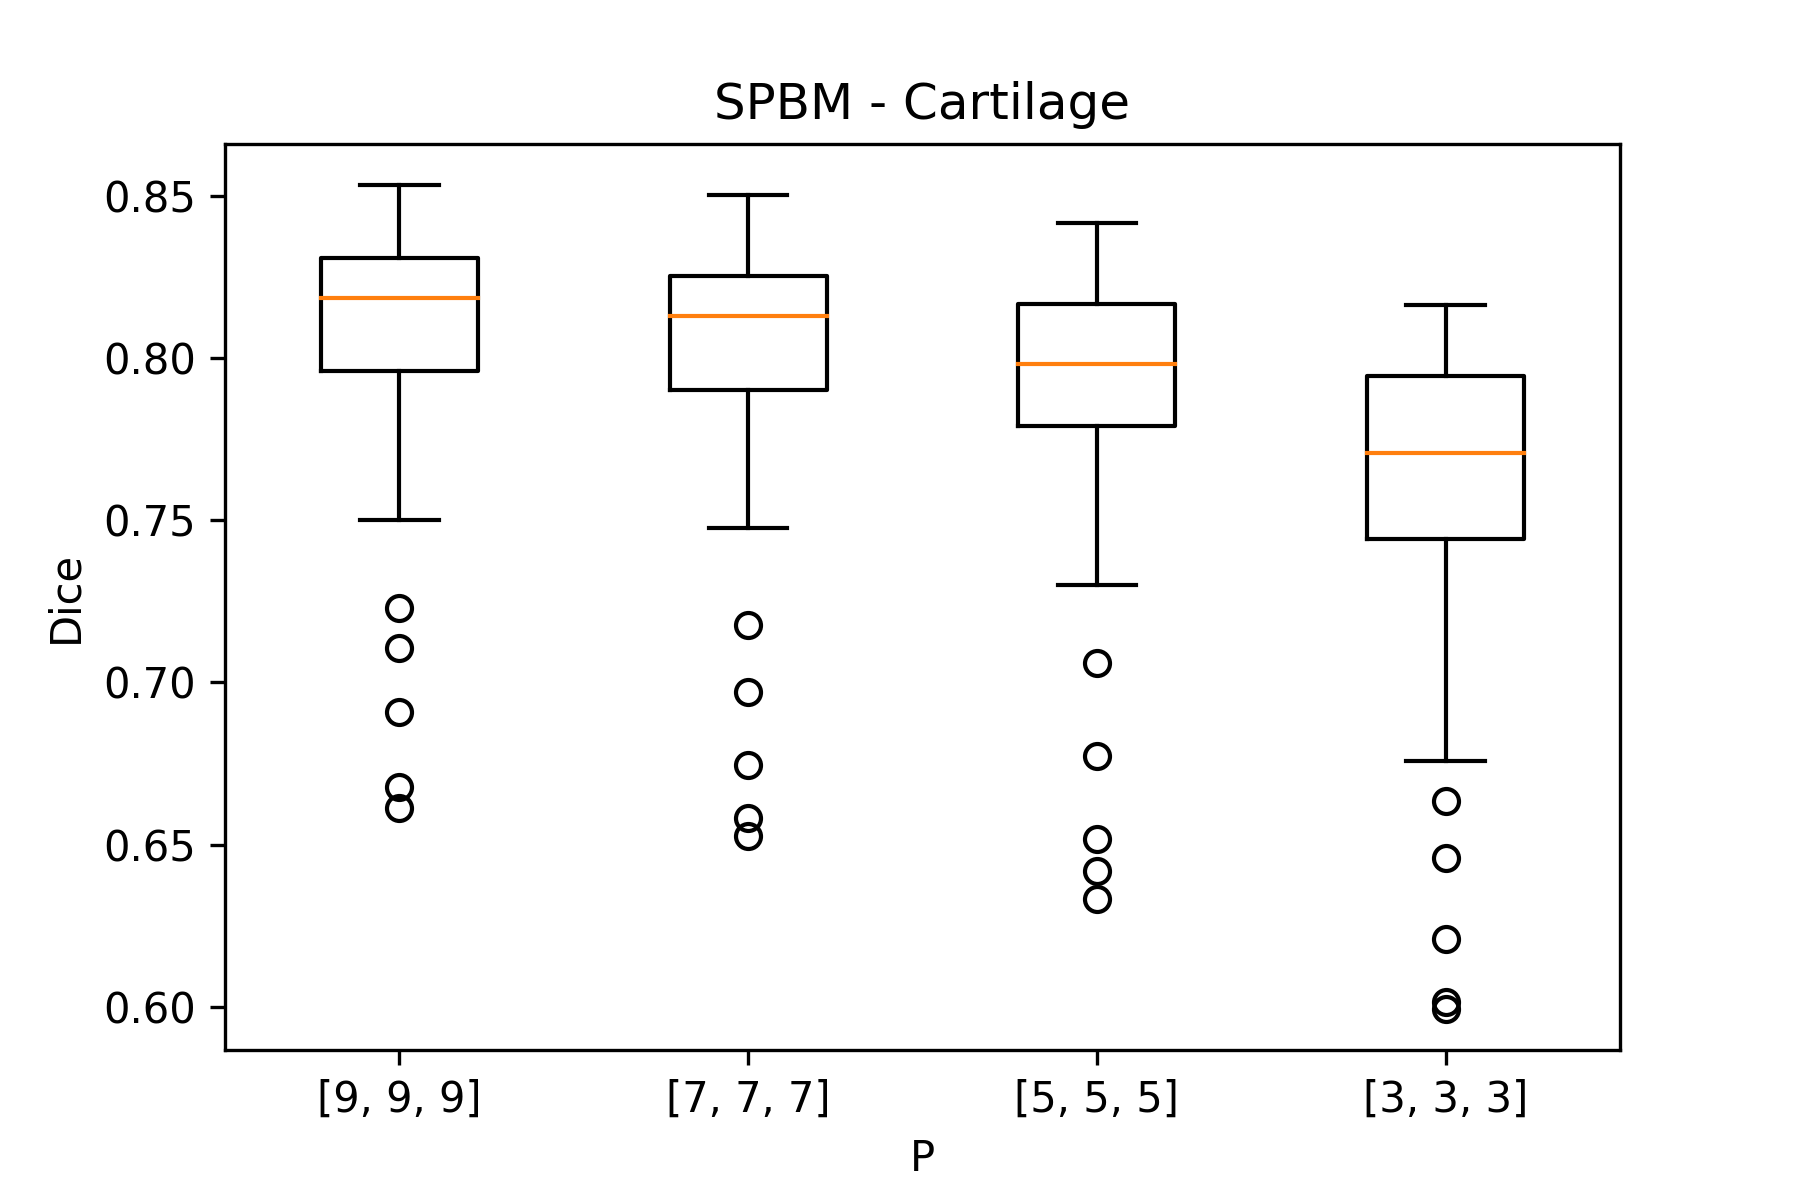
\includegraphics[width=\linewidth]{SPBM_P_Cartilage_plot.png}
    \caption{Χόνδροι}
    \end{subfigure}
    \begin{subfigure}[b]{0.42\linewidth}
        \begin{tabular}[t]{|l|c|} 
            \multicolumn{2}{c}{\footnotesize Σταθερές παράμετροι} \\
            \hline
            \footnotesize Παράμετρος $\lambda$ & \footnotesize 0.01 \\
            \hline
            \footnotesize Μέγεθος περιοχής αναζήτησης & \footnotesize  [3,3,3] \\ 
            \hline
            \footnotesize Αριθμός ατλάντων & \footnotesize 4 \\ 
            \hline
            \multicolumn{2}{c}{\footnotesize Επιλογή παραμέτρου} \\
            \hline
            \footnotesize Μέγεθος patch & \footnotesize [9,9,9] \\
            \hline
        \end{tabular}
    \caption{Παράμετροι}
    \end{subfigure}
\end{figure}

\end{frame}


\begin{frame}
\frametitle{Διασταυρωμένη επικύρωση του μεγέθους του patch}
\framesubtitle{Μέθοδος 2: Ταξινόμηση αραιής αναπαράστασης (SRC)}

\begin{figure}[H]
    \centering

    \begin{subfigure}[b]{0.42\linewidth}
    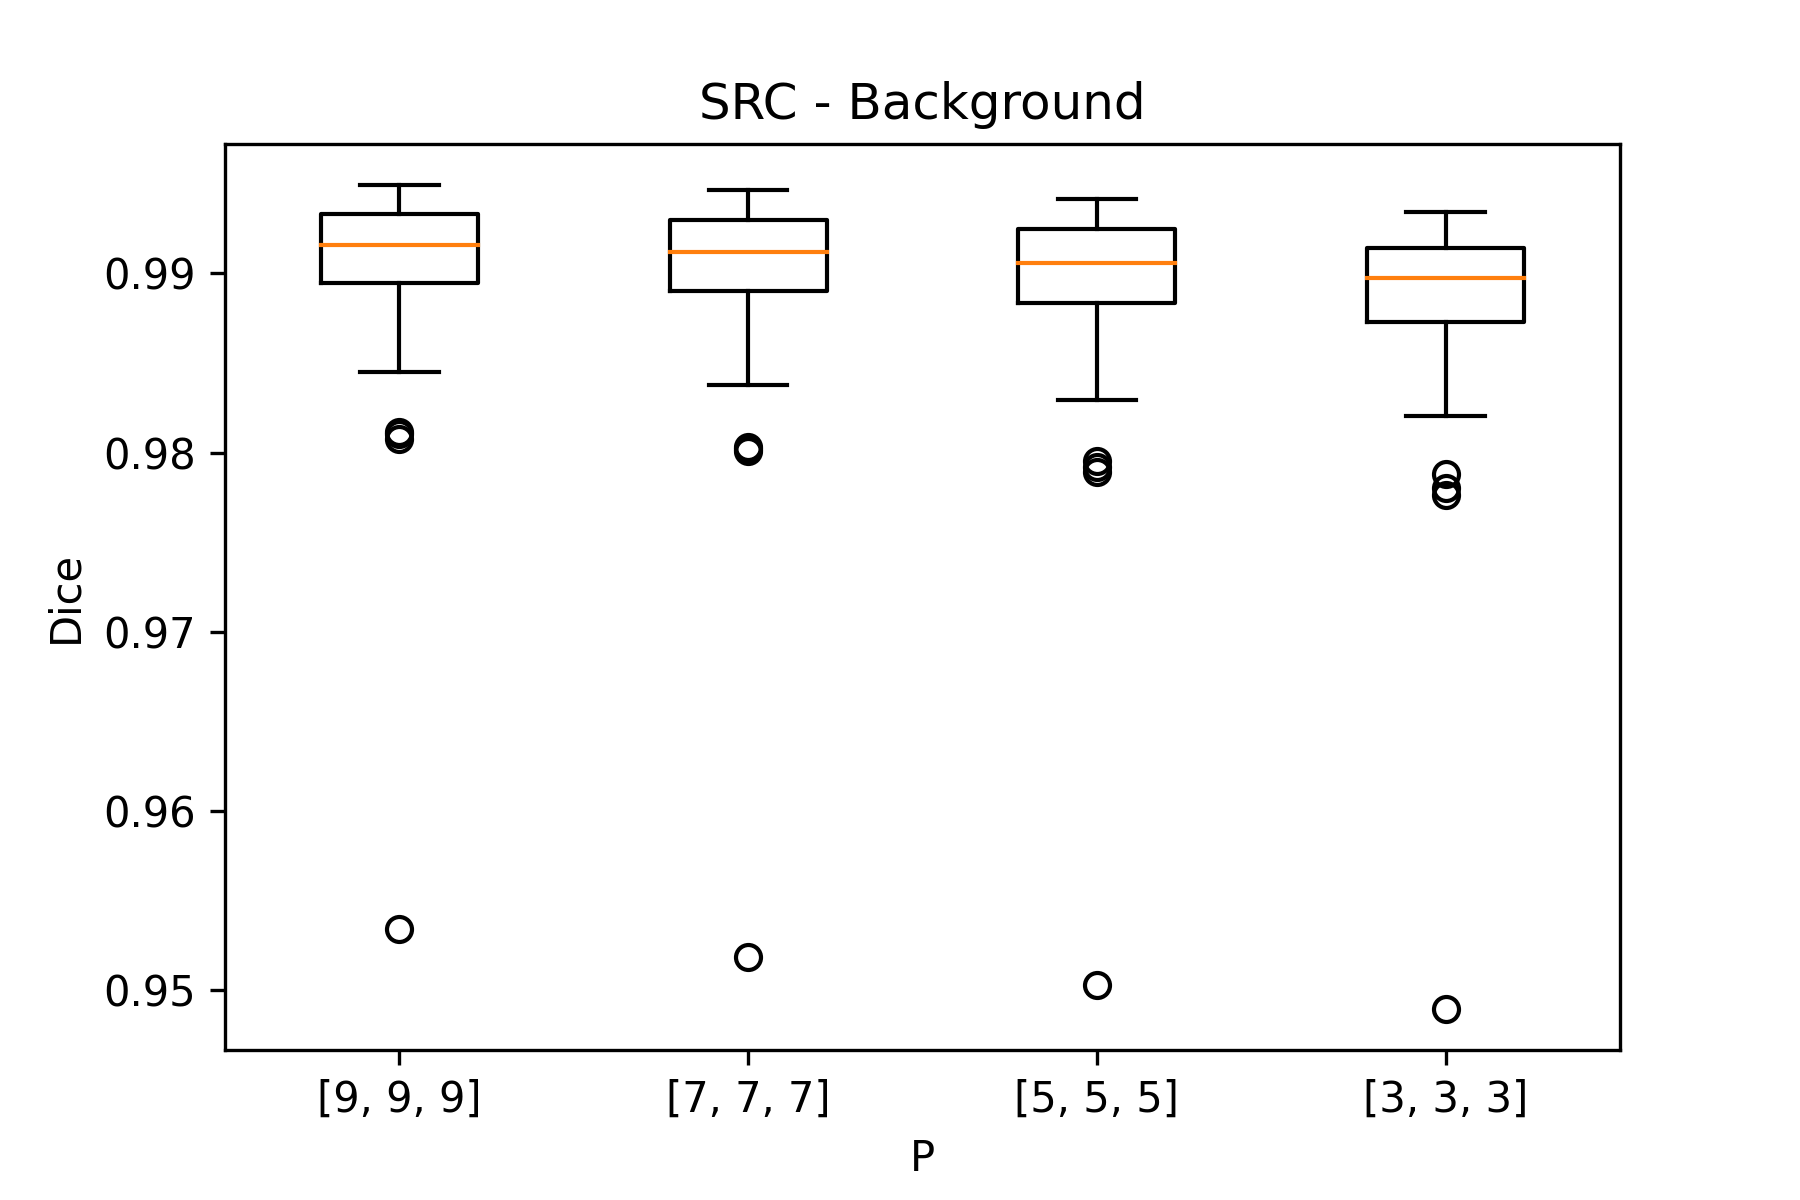
\includegraphics[width=\linewidth]{SRC_P_Background_plot.png}
    \caption{Παρασκήνιο}
    \end{subfigure}
    \begin{subfigure}[b]{0.42\linewidth}
    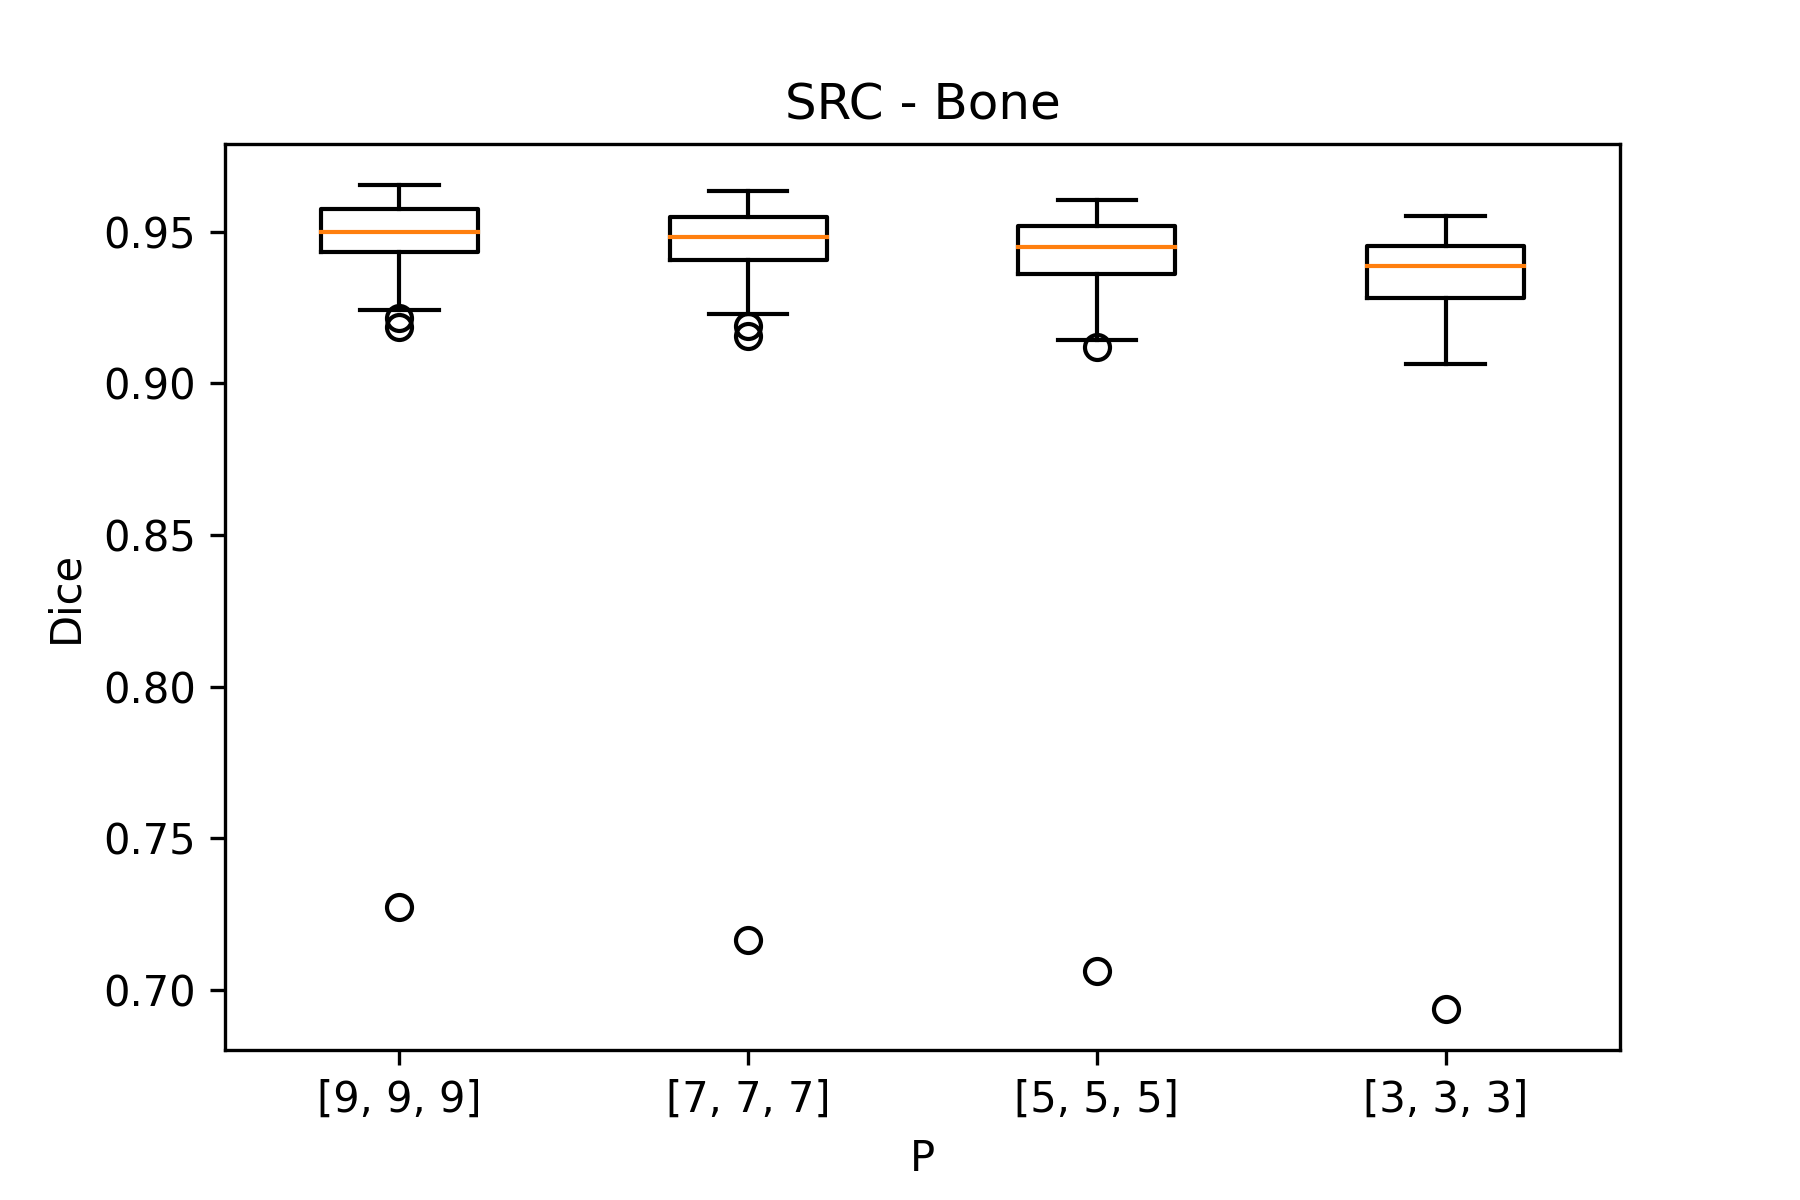
\includegraphics[width=\linewidth]{SRC_P_Bone_plot.png}
    \caption{Οστά}
    \end{subfigure}

    \begin{subfigure}[b]{0.42\linewidth}
    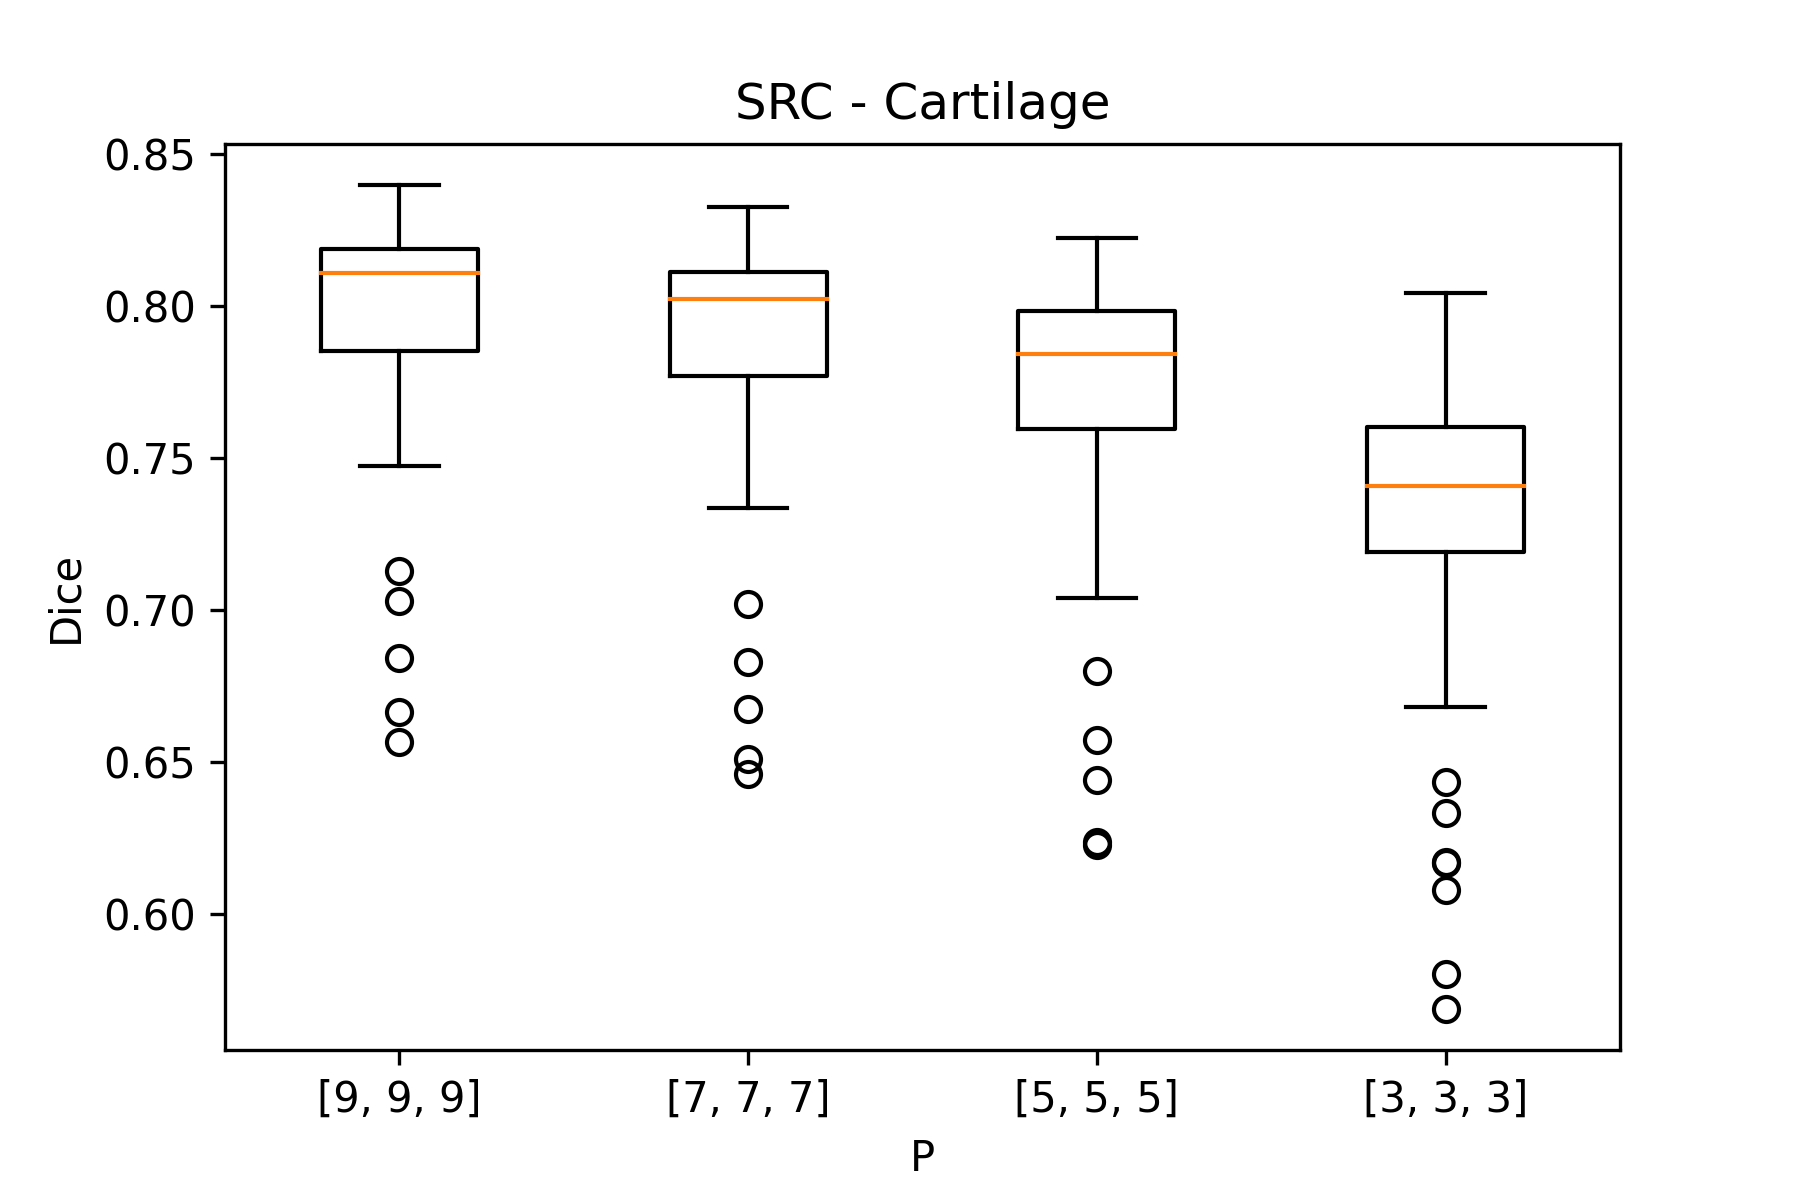
\includegraphics[width=\linewidth]{SRC_P_Cartilage_plot.png}
    \caption{Χόνδροι}
    \end{subfigure}
    \begin{subfigure}[b]{0.42\linewidth}
        \begin{tabular}[t]{|l|c|} 
            \multicolumn{2}{c}{\footnotesize Σταθερές παράμετροι} \\
            \hline
            \footnotesize Παράμετρος $\lambda$ & \footnotesize 0.1 \\
            \hline
            \footnotesize Μέγεθος περιοχής αναζήτησης & \footnotesize  [3,3,3] \\ 
            \hline
            \footnotesize Αριθμός ατλάντων & \footnotesize 4 \\ 
            \hline
            \multicolumn{2}{c}{\footnotesize Επιλογή παραμέτρου} \\
            \hline
            \footnotesize Μέγεθος patch & \footnotesize [9,9,9] \\
            \hline
        \end{tabular}
    \caption{Παράμετροι}
    \end{subfigure}
\end{figure}

\end{frame}


\begin{frame}
\frametitle{Διασταυρωμένη επικύρωση του μεγέθους του patch}
\framesubtitle{Μέθοδος 3: Κατάτμηση βασισμένη σε τμήματα με τη χρήση πληροφορίας
από ειδικούς (PBSEP)}

\begin{figure}[H]
    \centering

    \begin{subfigure}[b]{0.42\linewidth}
    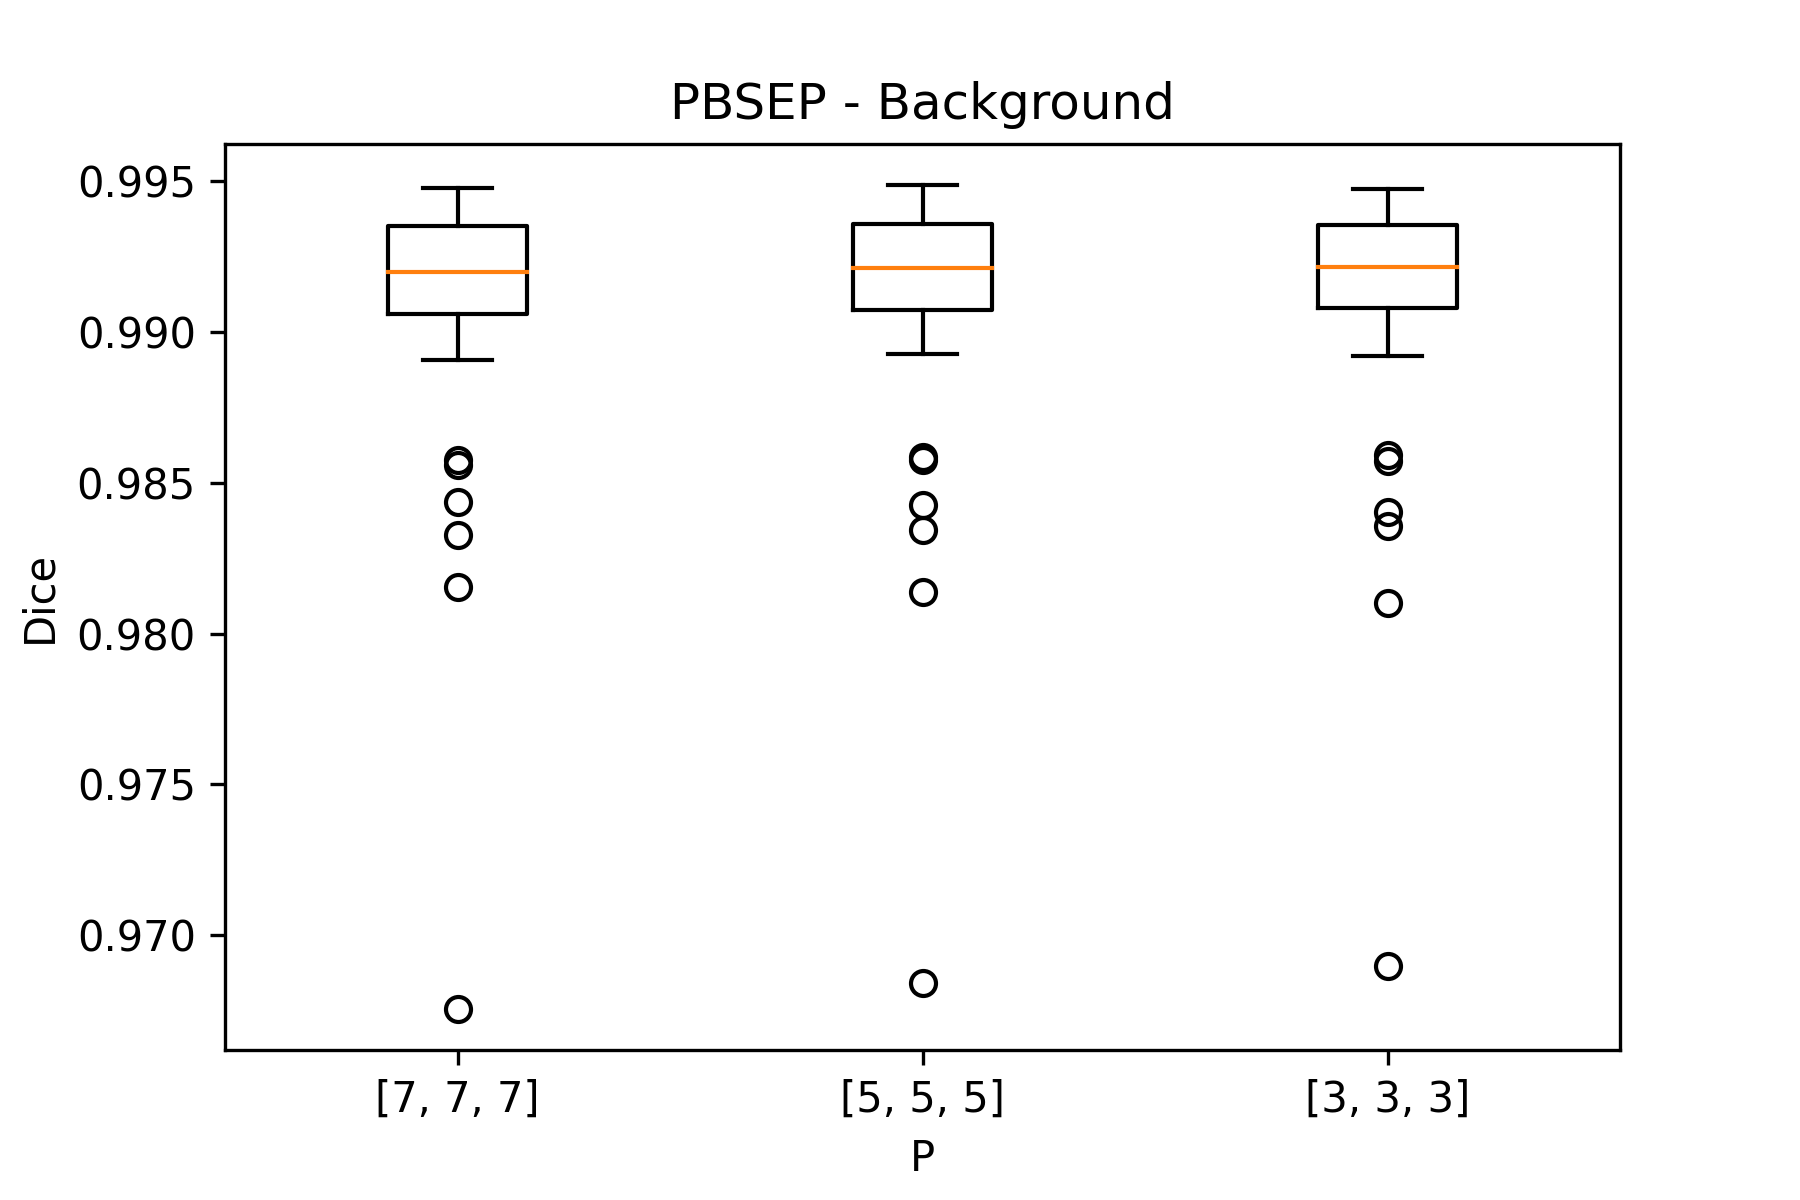
\includegraphics[width=\linewidth]{PBSEP_P_Background_plot.png}
    \caption{Παρασκήνιο}
    \end{subfigure}
    \begin{subfigure}[b]{0.42\linewidth}
    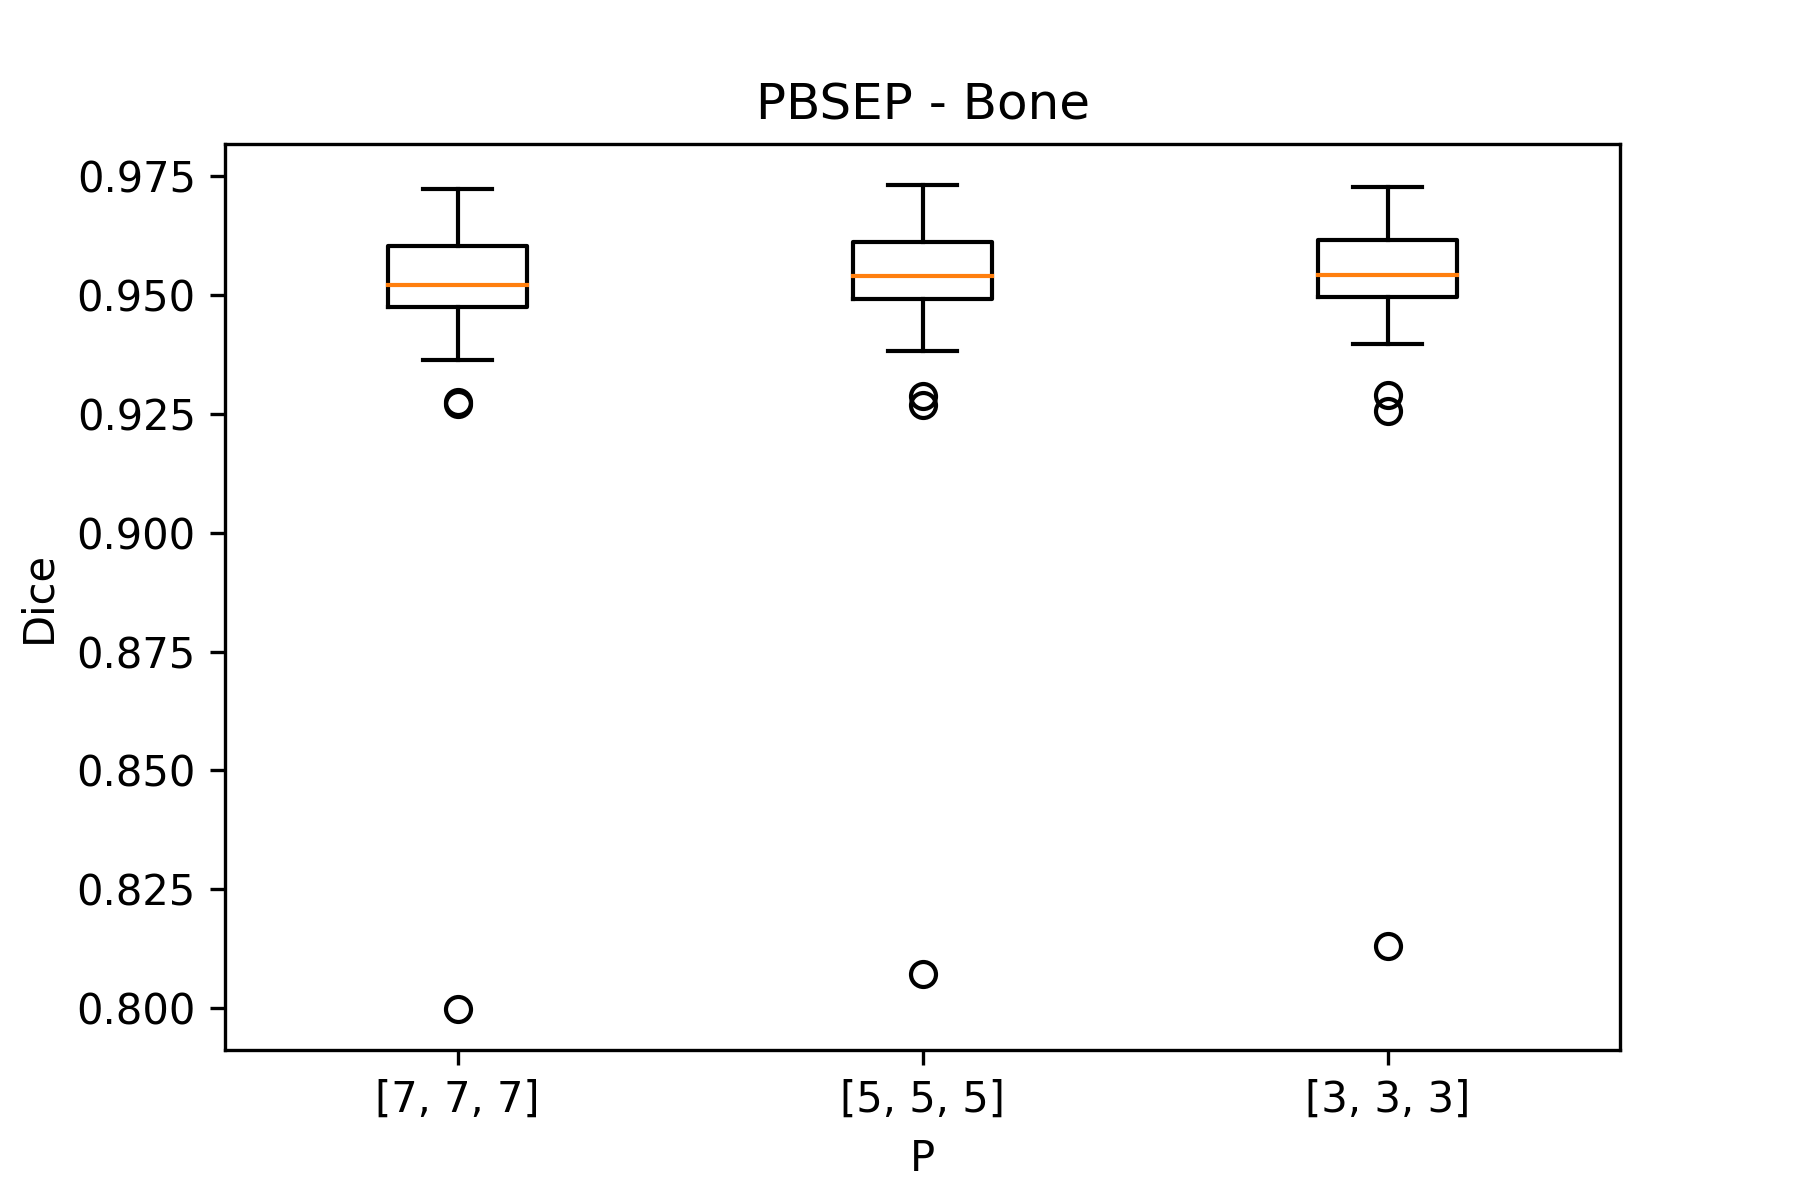
\includegraphics[width=\linewidth]{PBSEP_P_Bone_plot.png}
    \caption{Οστά}
    \end{subfigure}

    \begin{subfigure}[b]{0.42\linewidth}
    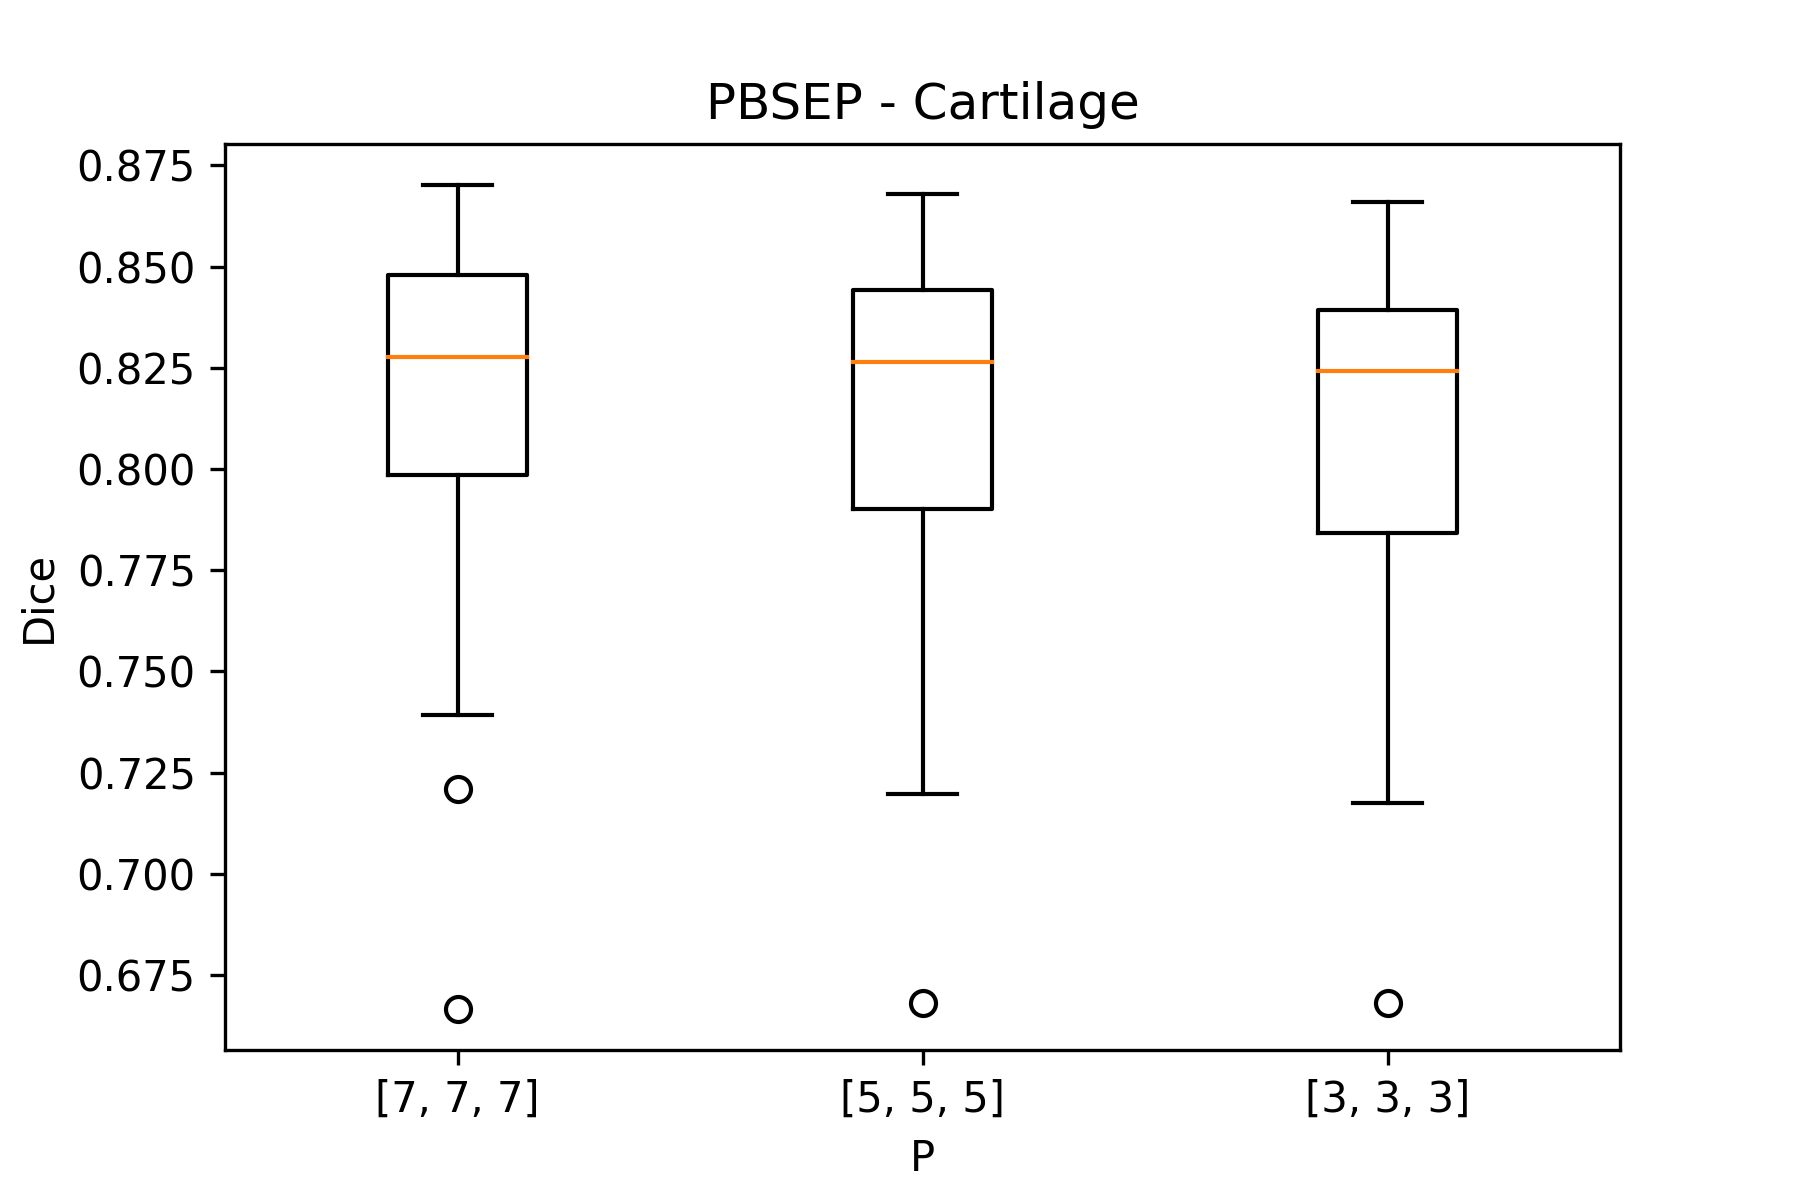
\includegraphics[width=\linewidth]{PBSEP_P_Cartilage_plot.png}
    \caption{Χόνδροι}
    \end{subfigure}
    \begin{subfigure}[b]{0.42\linewidth}
        \begin{tabular}[t]{|l|c|} 
            \multicolumn{2}{c}{\footnotesize Σταθερές παράμετροι} \\
            \hline
            \footnotesize Μέγεθος patch & \footnotesize [7,7,7] \\
            \hline
            \footnotesize Αριθμός ατλάντων & \footnotesize 4 \\ 
            \hline
            \multicolumn{2}{c}{\footnotesize Επιλογή παραμέτρου} \\
            \hline
            \footnotesize Μέγεθος περιοχής αναζήτησης & \footnotesize  [3,3,3] \\ 
            \hline
        \end{tabular}
    \caption{Παράμετροι}
    \end{subfigure}
\end{figure}

\end{frame}


\begin{frame}
\frametitle{Διασταυρωμένη επικύρωση του αριθμού των ατλάντων}
\framesubtitle{Μέθοδος 1: Αραιή μέθοδος βασισμένη σε τμήματα (SPBM)}

\begin{figure}[H]
    \centering

    \begin{subfigure}[b]{0.42\linewidth}
    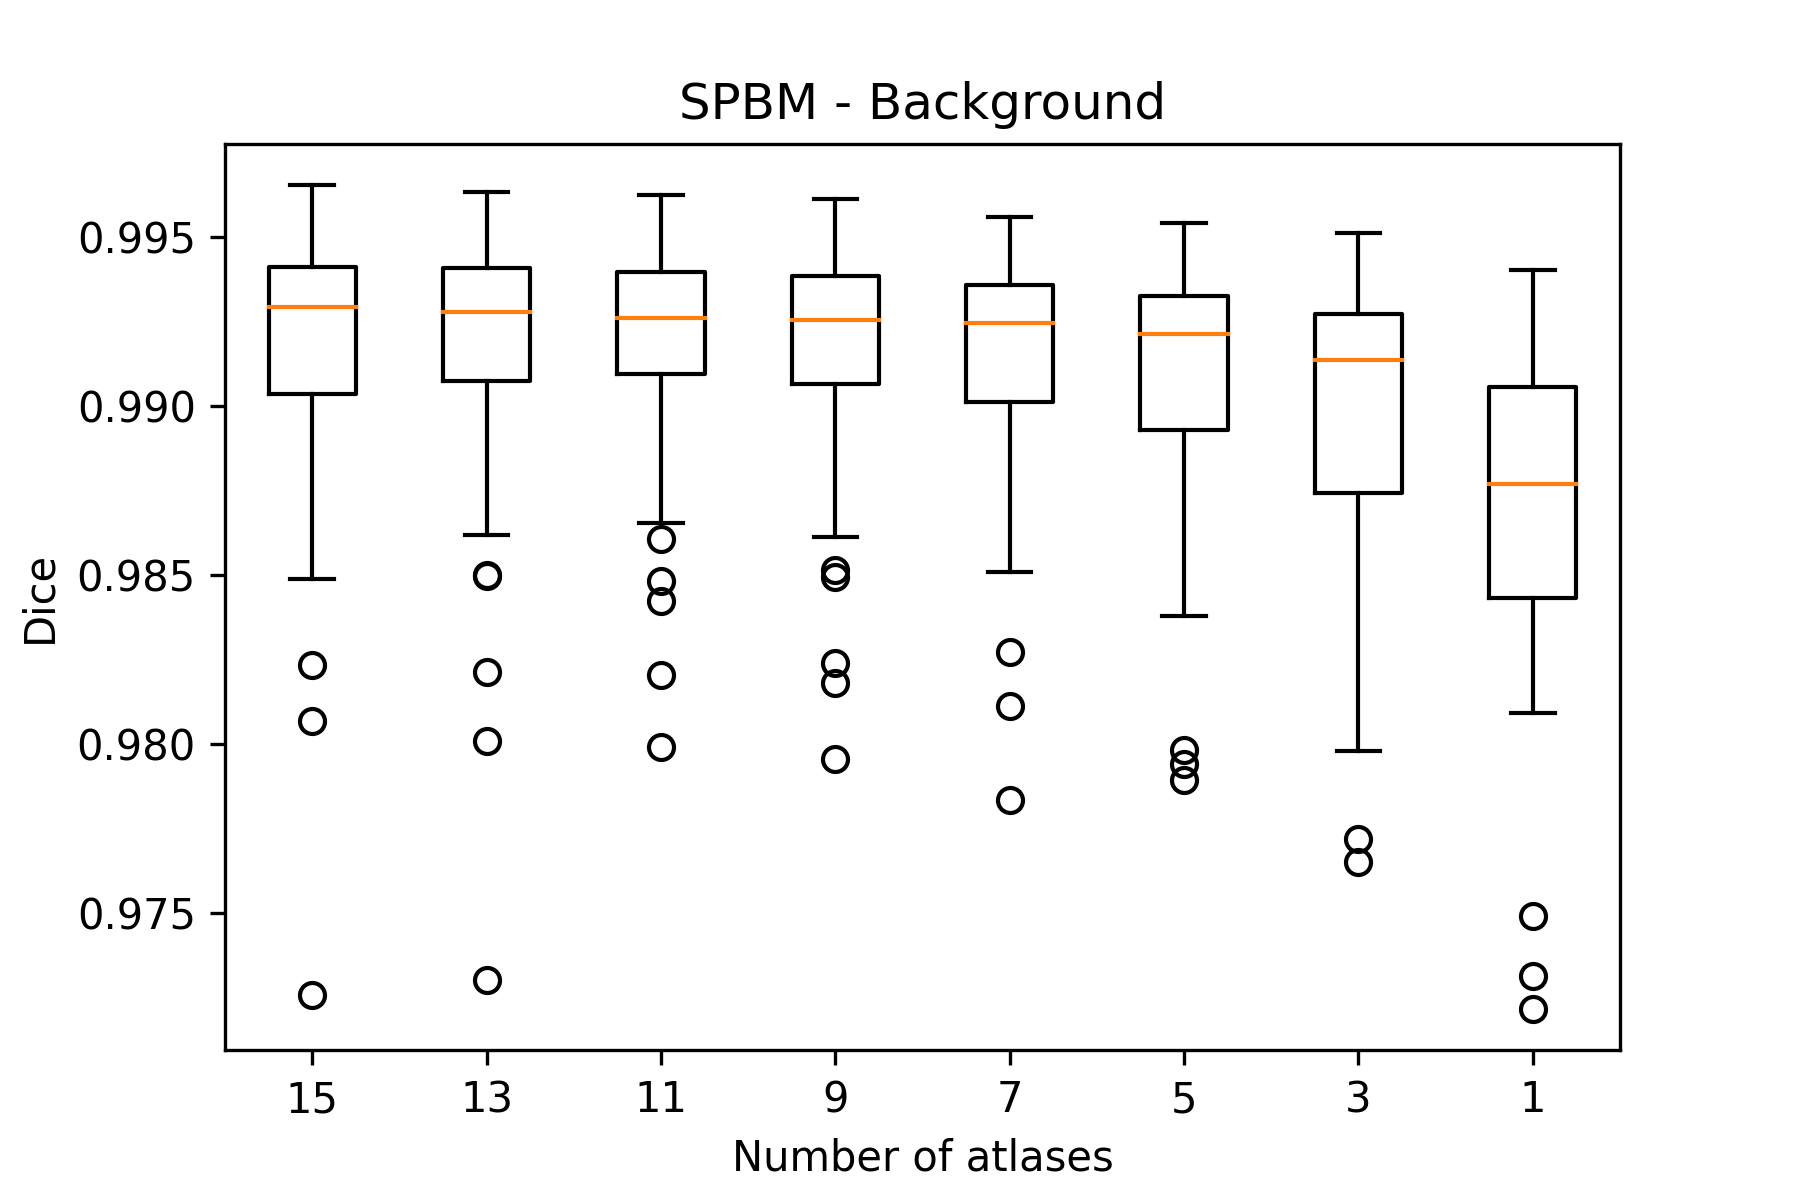
\includegraphics[width=\linewidth]{SPBM_Number_of_atlases_Background_plot.png}
    \caption{Παρασκήνιο}
    \end{subfigure}
    \begin{subfigure}[b]{0.42\linewidth}
    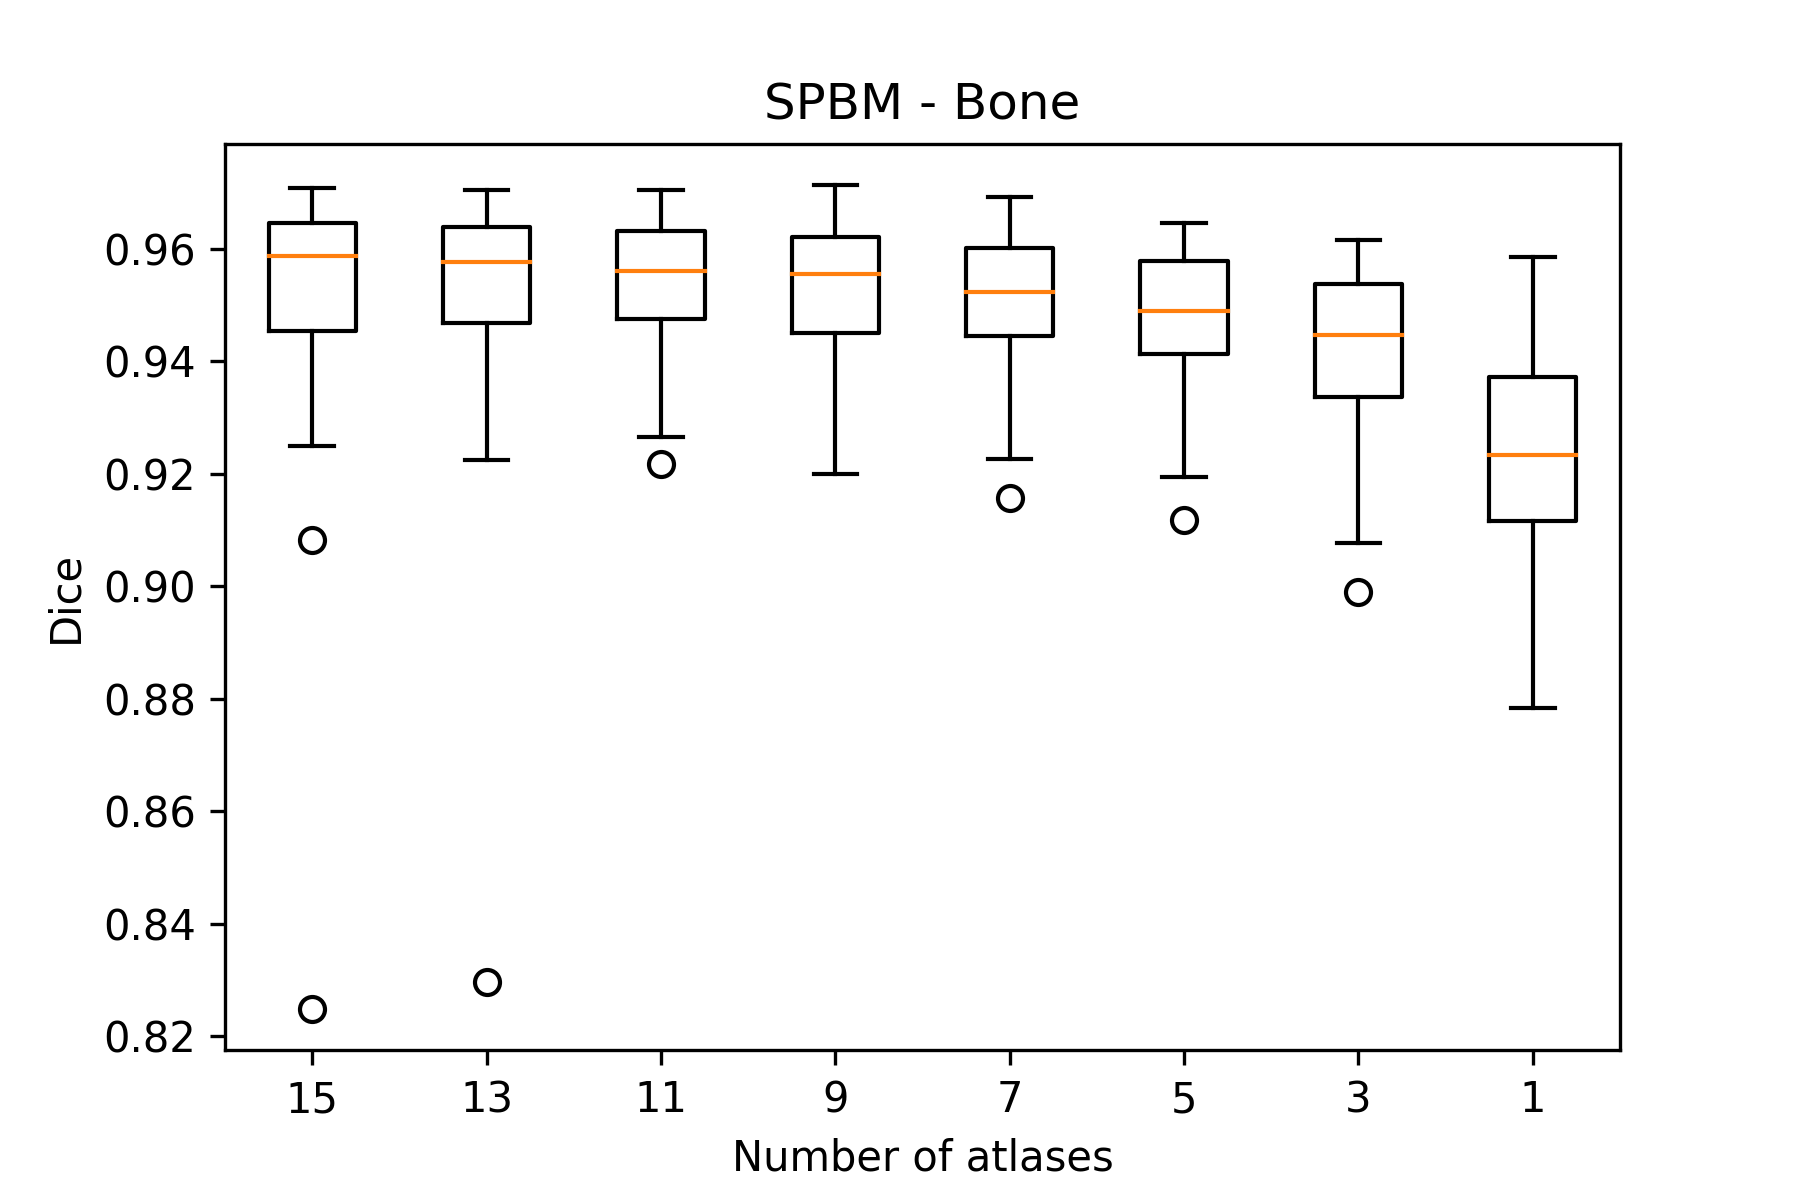
\includegraphics[width=\linewidth]{SPBM_Number_of_atlases_Bone_plot.png}
    \caption{Οστά}
    \end{subfigure}

    \begin{subfigure}[b]{0.42\linewidth}
    \includegraphics[width=\linewidth]{SPBM_Number_of_atlases_Cartilage_plot.png}
    \caption{Χόνδροι}
    \end{subfigure}
    \begin{subfigure}[b]{0.42\linewidth}
        \begin{tabular}[t]{|l|c|} 
            \multicolumn{2}{c}{\footnotesize Σταθερές παράμετροι} \\
            \hline
            \footnotesize Παράμετρος $\lambda$ & \footnotesize 0.01 \\
            \hline
            \footnotesize Μέγεθος περιοχής αναζήτησης & \footnotesize  [3,3,3] \\ 
            \hline
            \footnotesize Μέγεθος patch & \footnotesize [9,9,9] \\
            \hline
            \multicolumn{2}{c}{\footnotesize Επιλογή παραμέτρου} \\
            \hline
            \footnotesize Αριθμός ατλάντων & \footnotesize 9 \\ 
            \hline
        \end{tabular}
    \caption{Παράμετροι}
    \end{subfigure}
\end{figure}

\end{frame}


\begin{frame}
\frametitle{Διασταυρωμένη επικύρωση του αριθμού των ατλάντων}
\framesubtitle{Μέθοδος 2: Ταξινόμηση αραιής αναπαράστασης (SRC)}

\begin{figure}[H]
    \centering

    \begin{subfigure}[b]{0.42\linewidth}
    \includegraphics[width=\linewidth]{SRC_Number_of_atlases_Background_plot.png}
    \caption{Παρασκήνιο}
    \end{subfigure}
    \begin{subfigure}[b]{0.42\linewidth}
    \includegraphics[width=\linewidth]{SRC_Number_of_atlases_Bone_plot.png}
    \caption{Οστά}
    \end{subfigure}

    \begin{subfigure}[b]{0.42\linewidth}
    \includegraphics[width=\linewidth]{SRC_Number_of_atlases_Cartilage_plot.png}
    \caption{Χόνδροι}
    \end{subfigure}
    \begin{subfigure}[b]{0.42\linewidth}
        \begin{tabular}[t]{|l|c|} 
            \multicolumn{2}{c}{\footnotesize Σταθερές παράμετροι} \\
            \hline
            \footnotesize Παράμετρος $\lambda$ & \footnotesize 0.1 \\
            \hline
            \footnotesize Μέγεθος περιοχής αναζήτησης & \footnotesize  [3,3,3] \\ 
            \hline
            \footnotesize Μέγεθος patch & \footnotesize [9,9,9] \\
            \hline
            \multicolumn{2}{c}{\footnotesize Επιλογή παραμέτρου} \\
            \hline
            \footnotesize Αριθμός ατλάντων & \footnotesize 9 \\ 
            \hline
        \end{tabular}
    \caption{Παράμετροι}
    \end{subfigure}
\end{figure}

\end{frame}


\begin{frame}
\frametitle{Διασταυρωμένη επικύρωση του αριθμού των ατλάντων}
\framesubtitle{Μέθοδος 3: Κατάτμηση βασισμένη σε τμήματα με τη χρήση πληροφορίας
από ειδικούς (PBSEP)}

\begin{figure}[H]
    \centering

    \begin{subfigure}[b]{0.42\linewidth}
    \includegraphics[width=\linewidth]{PBSEP_Number_of_atlases_Background_plot.png}
    \caption{Παρασκήνιο}
    \end{subfigure}
    \begin{subfigure}[b]{0.42\linewidth}
    \includegraphics[width=\linewidth]{PBSEP_Number_of_atlases_Bone_plot.png}
    \caption{Οστά}
    \end{subfigure}

    \begin{subfigure}[b]{0.42\linewidth}
    \includegraphics[width=\linewidth]{PBSEP_Number_of_atlases_Cartilage_plot.png}
    \caption{Χόνδροι}
    \end{subfigure}
    \begin{subfigure}[b]{0.42\linewidth}
        \begin{tabular}[t]{|l|c|} 
            \multicolumn{2}{c}{\footnotesize Σταθερές παράμετροι} \\
            \hline
            \footnotesize Μέγεθος περιοχής αναζήτησης & \footnotesize  [7,7,7] \\ 
            \hline
            \footnotesize Μέγεθος patch & \footnotesize [3,3,3] \\
            \hline
            \multicolumn{2}{c}{\footnotesize Επιλογή παραμέτρου} \\
            \hline
            \footnotesize Αριθμός ατλάντων & \footnotesize 9 \\ 
            \hline
        \end{tabular}
    \caption{Παράμετροι}
    \end{subfigure}
\end{figure}

\end{frame}


\section{Σύγκριση μεθόδων}
\subsection{Σύγκριση απόδοσης μεθόδων}

\begin{frame}
\frametitle{Σύγκριση απόδοσης μεθόδων}
\framesubtitle{Διαγράμματα}

\begin{figure}[H]
    \centering

    \begin{subfigure}[b]{0.42\linewidth}
    \includegraphics[width=\linewidth]{Dice_final_Background_plot.png}
    \caption{Παρασκήνιο}
    \end{subfigure}
    \begin{subfigure}[b]{0.42\linewidth}
    \includegraphics[width=\linewidth]{Dice_final_Bone_plot.png}
    \caption{Οστά}
    \end{subfigure}

    \begin{subfigure}[b]{0.42\linewidth}
    \includegraphics[width=\linewidth]{Dice_final_Cartilage_plot.png}
    \caption{Χόνδροι}
    \end{subfigure}
\end{figure}

\end{frame}


\begin{frame}
\frametitle{Σύγκριση απόδοσης μεθόδων}
\framesubtitle{Στατιστικά}

\begin{table}[h!]
    \centering
    \begin{tabular}{|c|c||c|c|} 
        \hline
        Μέθοδος & Ετικέτα & Μέσος όρος & Διάμεσος \\ 
        \hline
        \hline
        \multirow{3}{4em}{SPBM} & Παρασκήνιο & 0.9914 & 0.9926 \\ 
        & Οστά & 0.9521 & 0.9556 \\ 
        & Χόνδροι & 0.8209 & 0.8352 \\ 
        \hline
        \multirow{3}{4em}{SRC} & Παρασκήνιο & 0.9914 & 0.9926 \\ 
        & Οστά & 0.9528 & 0.9585 \\ 
        & Χόνδροι & 0.8056 & 0.8187 \\ 
        \hline
        \multirow{3}{4em}{PBSEP} & Παρασκήνιο & 0.9916 & 0.9933 \\ 
        & Οστά & 0.956 & 0.9624 \\ 
        & Χόνδροι & 0.8281 & 0.8451 \\ 
        \hline
    \end{tabular}
    \caption{Μέσος όρος και διάμεσος του συντελεστή ομοιότητας Dice για όλες
             τις μεθόδους και ετικέτες.}
\end{table}

\end{frame}


\subsection{Σύγκριση χρόνου εκτέλεσης}


\begin{frame}
\frametitle{Σύγκριση χρόνου εκτέλεσης}

\begin{figure}[H]
    \centering

    \begin{subfigure}[b]{0.38\linewidth}
    \includegraphics[width=\linewidth]{Registration_time_plot.png}
    \caption{Χρόνος καταχώρησης}
    \end{subfigure}
    \begin{subfigure}[b]{0.38\linewidth}
    \includegraphics[width=\linewidth]{Segmentation_time_plot.png}
    \caption{Χρόνος κατάτμησης}
    \end{subfigure}

    \begin{subfigure}[b]{0.38\linewidth}
    \includegraphics[width=\linewidth]{Total_time_plot.png}
    \caption{Συνολικός χρόνος}
    \end{subfigure}
\end{figure}

\tiny
* Τα πειράματα έτρεξαν σε υπολογιστή με επεξεργαστή τον \emph{Intel(R) Core(TM)
i9-7940X CPU @ 3.10GHz} και \emph{126GB} μνήμη. Κάθε πείραμα έτρεχε σε ένα νήμα
(thread) και για τον υπολογισμό των χρόνων έτρεχαν παράλληλα \emph{14} νήματα
(ένα για κάθε πείραμα).

\end{frame}


\section{Ερωτήσεις}


\begin{frame}
\frametitle{Ερωτήσεις}

\begin{figure}[H]
    \centering
    \includegraphics[height=0.8\textheight]{question_mark}
\end{figure}


\end{frame}









\end{document}
